%!TEX TS-program = xelatex
%!TEX encoding = UTF-8 Unicode
\PassOptionsToPackage{svgnames}{xcolor} % https://tex.stackexchange.com/questions/653681/how-to-use-xcolor-color-names-in-tikzpicture-style deve essere messo prima di \documentclass{}
% Load Thesis Class
\documentclass{PODThesis}

\title{Emulating Cosmological Likelihoods with Machine Learning}

\author{Marco Giunta}
\studentId{2025169}

% Advisor
\advisor{Prof. Michele Liguori}

% If you are co-advised
\coadvisor{Prof. Marco Raveri}
\coadvisorsUniversity{University of Genova}

\university{University of Padova}
\mastername{Physics of Data}
\academicYear{2022/2023}

\begin{filecontents*}[overwrite]{\jobname.xmpdata}
    \Title{Emulating Cosmological Likelihoods with Machine Learning}
    \Author{Marco Giunta}
    \Language{en-EN}
    \Keywords{Physics of Data\sep LaTeX}
\end{filecontents*}

\renewcommand{\L}{\mathcal{L}}
\usepackage{float}
\usepackage{comment}
\usepackage{amsthm}
\theoremstyle{definition}
\newtheorem*{definition}{Definition}

\usetikzlibrary{positioning}
%\PassOptionsToPackage{svgnames}{xcolor} % x11names
\forestset{
    .style={
        for tree={
            base=bottom,
            child anchor=north,
            align=center,
            s sep+=1cm,
    straight edge/.style={
        edge path={\noexpand\path[\forestoption{edge},thick,-{Latex}] 
        (!u.parent anchor) -- (.child anchor);}
    },
    if n children={0}
        {tier=word, draw, thick, rectangle}
        {draw, diamond, thick, aspect=2},
    if n=1{%
        edge path={\noexpand\path[\forestoption{edge},thick,-{Latex}] 
        (!u.parent anchor) -| (.child anchor) node[pos=.2, above] {Y};}
        }{
        edge path={\noexpand\path[\forestoption{edge},thick,-{Latex}] 
        (!u.parent anchor) -| (.child anchor) node[pos=.2, above] {N};}
        }
        }
    }
}

%\newcommand{\cosmolime}{\textsc{CosmoLIME}} % Nota lo spazio! per qualche motivo lo spazio è necessario... usando direttamente \textsc(CosmoLIME) non ci sono problemi, invece con \cosmolime lo spazio serve

% Document

\begin{document}
    % The front matter (Cover, ToC, Abstract, etc...)
    \frontmatter

    % The main content
    \mainmatter
    
    %\include{chapters/01_introduction}
    %\include{chapters/02_stateofart}
    %\include{chapters/03_background}
    %\include{chapters/04_analysis}
    %\include{chapters/99_conclusions}

    \chapter{Introduction}

%\section{Bayesian Inference in modern science} % troppo lavoro e a me qui basta riassumere i passaggi

%inferenza bayesiana (figura semplice prior -> likelihood -> posterior), emulatori non cosmologici tipo speculator, emulatori cosmologici tipo cosmopower, ma sono tutti statici

%TEST CITAZIONE: \cite{cosmopower} \cite{precision_ml} \cite{islp} \cite{likelihood_cmb} \cite{understanding_ml} \cite{modern_cosmology}

% \section{Bayesian Inference Recap}
% \subsection{Bayesian Parameter Inference in Cosmology}

% \section{Bayesian Parameter Inference in Cosmology} % ancora non si parla molto di cosmologia qua...
\section{Bayesian Parameter Inference}
\subsection{Bayesian Parameter Inference: Conceptual Recap}
Bayesian methods have become a staple of modern science - and rightfully so, as they make the process of learning from data intuitive and rigorous; thanks to Bayes' theorem with only probability theory one can tackle common problems - such as parameter inference or model comparison - using a general, well-grounded approach. A Bayesian analysis is usually easier to interpret compared to its frequentist counterpart: the concept of probabilities as degrees of certainty about statements about the world is quite intuitive, and offers many other advantages - e.g. it removes the need to study the outcomes of other imaginary experiments one could have done. The main disadvantage of the Bayesian approach - i.e. the need for expensive computations - has stopped being an insurmountable obstacle in the era of cheap and powerful computers; still the computational side of a Bayesian analysis can pose nontrivial challenges, especially since in the last few decades the dimensionality of parameter spaces over which relevant posterior are defined has increased exponentially.
In particular in the context of cosmology there are peculiar computational challenges in applying Bayes' theorem: due to the unique properties of the problem at hand special tools have been developed to accelerate expensive analyses; in order to discuss these issues let us first recap the basic ingredients of a Bayesian analysis.

In the following we focus on the problem of parameter inference, i.e. trying to indirectly measure the value of some model parameters given a dataset about something else; even though the machinery of Bayesian statistics can also be applied to other problems (such as model selection) parameter inference is arguably both the simplest and most common scenario where one applies these tools. Parameter inference is usually the situation where students first familiarize themselves with Bayesian statistics, and is also especially relevant in cosmology, since inferring cosmological parameters from data about astrophysical objects is ``one of the cornerstones of modern observational cosmology'' \cite{cosmopower}. Finally we remark that the main topic of this thesis i.e. emulators in cosmology is about accelerating parameter inference pipelines - hence why we restrict our attention to this subset of what Bayesian statistics has to offer.

% \subsection{Inferring Parameters in Practice}
\subsection{Bayesian Parameter Inference: Practical Recap}
The starting point of the Bayesian approach to statistics is to treat model parameters as random variables and the available dataset as fixed. This reflects the idea that the dataset is just given to us, while with model parameters we use the ``notation of probabilities to represent [our] \emph{beliefs} about the mutually exclusive micro-hypotheses (here, values of [the parameters]), of which only one is actually true.'' \cite{mckay}. The idea is to use probabilities to denote degrees of belief given assumptions - hence why we use probability distributions to capture what we know about e.g. the value of a parameter.

All Bayesian pipelines hinge in some way on \emph{Bayes' theorem}:
\begin{equation*}
    P(\theta|D) = \frac{P(D|\theta) P(\theta)}{P(D)}
\end{equation*}
where we assume we have a dataset $D$ and model parameters $\theta$; each of the above probability distributions has a special name and meaning.

\paragraph{Prior distribution}
The distribution $P(\theta)$ is the \emph{prior Distribution}, and it represents prior beliefs, i.e. all the assumptions we enforce on the parameters $\theta$ \emph{before} seeing the data $D$. The prior can be used to express previous knowledge (for example it can be the posterior of a previous experiment) or assumptions (for example a reasonable prior describing a particle mass should be zero for negative values); otherwise one can use a ``blank'' prior, i.e. a distribution trying to express lack of previous knowledge about the parameters. Defining a good prior can be challenging; for example trying to make a prior uninformative in a parameter can result in a highly informative prior in a function of that same parameter (see for example \cite{noninformative_priors} \cite{nsb_prior}) - resulting in a biased posterior, requiring a switch of prior or the acquisition of more data.

\paragraph{Likelihood distribution}
The distribution $P(D|\theta)$ is called the \emph{likelihood distribution}; since this term is the protagonist of this work it deserves to have a unique symbol, hence in what follows the notation $\L(D|\theta)$ will be used. The likelihood is the part that captures the \emph{model} chosen to describe the physical process at hand; it is defined as the probability (density) of observing the dataset $D$ given that the model parameters are equal to $\theta$, but in a Bayesian context one usually ``flips it around''. What this means is that the expression of the likelihood is obtained as the probability of observing a dataset conditioned on known parameters, but then we fix the dataset equal to the obtained data samples and treat the likelihood as a function of the model parameters. Usually the likelihood contains both the physical model (a description of the part we actually care about) and the noise model (a description of the part we would like to remove but cannot), which requires one to have both relevant and nuisance parameters - the latter of which can be rigorously dealt with in a Bayesian setting thanks to marginalization.

\paragraph{Evidence}
The $P(D)$ term is called the \emph{evidence}. Even though in some problems its value plays a significant role (e.g. in model selection) in parameter inference it simply serves the purpose of regularizing the product of prior and likelihood, i.e. it ensures the resulting distribution's integral over all possible parameter values is 1. Indeed due to the rules of probability one can trivially check that the product of likelihood and prior is simply the joint probability distribution over $\theta$ and $D$, therefore its integral w.r.t. $\theta$ simply results in the marginal $P(D)$ - ensuring the ratio in the R.H.S. of Bayes' theorem is properly normalized. This marginalization makes it clear that the evidence represents the probability of observing the data irrespective of the value of the values of model parameters, i.e. this quantity is the union of all events leading to the dataset $D$ at hand - each with its own value of $\theta$.

Since the evidence is to be computed by integrating in parameter space over all possible $\theta$ value it becomes apparent that when the number of parameters is large (as has become more and more common over the last decades) this term can be basically impossible to compute; specialized techniques relying on \emph{Markov Chain Monte Carlo} methods have been developed to surmount the need to compute this quantity.

\paragraph{Posterior distribution}
The distribution $P(\theta|D)$ is called the \emph{posterior distribution}, and is the target of Bayesian inference. This distribution represents the updated beliefs about the parameters, \emph{after} learning from the data. The whole point of inference is to move from the prior to the posterior, i.e. to incorporate new knowledge about the world and let it modify previous beliefs. Superficially it seems as if the posterior distribution can be trivially obtained from Bayes' theorem once the prior and likelihood have been provided; in practice, though, this can be computationally expensive in all but the simplest of analyses. For example the evidence may be impossible to compute directly and indirect techniques may be needed, as described above; another common issue is that sometimes the likelihood is expensive to exactly evaluate, slowing down the whole pipeline process - hence why ``likelihood-free'' methods have found success in situations where the likelihood is expensive to evaluate but cheap to sample from (see \cite{astroabc} for a relevant cosmological example), which are common e.g. when the exact likelihood expression is known but requires an expensive normalization factor.

Once the posterior has been obtained it contains everything we could possibly want to know about the parameters; for example via marginalization we can obtain compact estimates for each parameter, we can compute credible regions, etc.

\subsubsection{Learning with Bayes' theorem}
The process of learning from data with a Bayesian parameter inference can be schematized as follows:
\begin{equation*}
    \text{Prior} \ P(\theta) \to \text{Likelihood} \ \L(D|\theta) \to \text{Posterior} \ P(\theta|D)
\end{equation*}
Paraphrasing the words of McKay \cite{mckay}:
\begin{quote}
    What you know about $\theta$ after the data arrive ($P(\theta|D)$) is what you knew before ($P(\theta)$), and what the data told you ($\L(D|\theta)$).
\end{quote}
The beautiful thing about Bayes' theorem is that it provides a way to intuitively and rigorously model mathematically the process of learning new knowledge about the state of the world, only relying on probability theory - therefore without the need to have a bunch of ad hoc tests and methods to come up with an answer about something.
Quoting \cite{doing_bayesian_data_analysis}:
\begin{quote}
    In summary, the essence of Bayesian inference is reallocation of credibility across possibilities. The distribution of credibility initially reflects prior knowledge about the possibilities, which can be quite vague. Then new data are observed, and the credibility is re-allocated. Possibilities that are consistent with the data garner more credibility, while possibilities that are not consistent with the data lose credibility. Bayesian analysis is the mathematics of re-allocating credibility in a logically coherent and precise way.
\end{quote}
% establish basic notation, scratch the surface...
Of course this discussion barely scratched the surface of what Bayes' theorem has to offer, both in theory and in practice. The point of this introduction is mostly to establish some basic notation and terminology that will be used extensively throughout the present work. The eager reader may find great resources about Bayesian analysis in \cite{mckay}, \cite{doing_bayesian_data_analysis}, \cite{jaynes_mysteries}, \cite{data_analysis_bayesian}, with \cite{trotta_sito} and \cite{trotta2017bayesian} being geared towards cosmology in particular.

\section{Emulators in Cosmology}
\subsection{Likelihood Emulation in Cosmology}
%descrivi a cosa servono e fai esempi di emulatori preesistenti
As described above in order to obtain a posterior one must be able to evaluate the appropriate likelihood - which can be computationally expensive. In particular in cosmology much work has been dedicated to the analysis of two-point statistics (power spectra or correlation functions); while this is appropriate (these observables carry a lot of information about cosmological parameters) it forces one to compute e.g. the theoretical power spectra corresponding to a given cosmological model i.e. a given set of values of the cosmological parameters. Indeed in inference pipelines of this kind the computational bottleneck is running exact Boltzmann solvers like \texttt{camb} \cite{camb} or \texttt{class} \cite{class_1} \cite{class_2}. A remarkable property of these spectra is that exact evaluations with repeated, expensive calls to these codes is often avoidable: \emph{in general cosmological power spectra are smooth functions of their input parameters} - hence why in the last 20 years many \emph{cosmological emulators} have been developed, i.e. fast and accurate surrogate functions that map cosmological parameters to the corresponding predicted power spectra.

\begin{equation*}
    \theta \mapsto P(\theta)
\end{equation*}
The idea is simple: since the above mapping between cosmological parameters and theoretical power spectra is usually regular, stable and smooth one can simulate a dataset of $(\theta, P(\theta))$ pairs (i.e. parameters values-corresponding spectra), then train an algorithm to learn this mapping as accurately as possible. It will then be possible to replace the expensive call to a Boltzmann solver with a quick one to the emulator: if training is successful the algorithm will both be able to reproduce spectra already presented to it (i.e. remember the dataset) and to accurately compute unseen before spectra, exploiting the smoothness of this mapping to fill the gaps in its knowledge of the $\theta \mapsto P(\theta)$ mapping (i.e. interpolate the dataset).
Thanks to emulation it becomes possible to have a once-and-for-all expensive training phase, after which power spectra can be obtained with a negligible loss in accuracy in the overall parameter inference with orders of magnitude speedups in the total computational overhead. 

The idea of accelerating inference pipelines with emulators has been successfully applied in many fields of science; this is especially true in the case of cosmology. The earliest successful attempts at emulation involved polynomial regression of power spectra \cite{emulator_poly_1} \cite{emulator_poly_2}; many emulators based on Gaussian Processes followed, applying these ideas to the emulation of matter power spectra \cite{emulator_gp_matter_1} \cite{emulator_gp_matter_2} \cite{emulator_gp_matter_3} \cite{emulator_gp_matter_4} \cite{emulator_gp_matter_5} \cite{emulator_gp_matter_6} \cite{emulator_gp_matter_7} \cite{emulator_gp_matter_8} \cite{emulator_gp_matter_9} \cite{emulator_gp_matter_10}, cosmic shear band powers \cite{emulator_gp_cosmic_shear_band_powers}, and Lyman-$\alpha$ forest flux power spectrum \cite{emulator_gp_lyman_1} \cite{emulator_gp_lyman_2}.
The recent surge in popularity of neural networks attracted the interest of the astrophysical community and ensured another batch of cosmological emulators relied on them - for the emulation of power spectra \cite{emulator_nn_matter_1} \cite{emulator_nn_matter_2} \cite{emulator_nn_matter_3} \cite{emulator_nn_matter_4} \cite{emulator_nn_matter_5} \cite{emulator_nn_matter_6}, angular power spectra of LSS observables \cite{emulator_nn_angular_lss}, global 21-cm signal \cite{emulator_nn_21_cm_1} \cite{emulator_nn_21_cm_2} \cite{emulator_nn_21_cm_3}, and to accelerate parts of Boltzmann codes \cite{emulator_nn_boltzmann}.
This list is clearly incomplete, as the literature is filled with several approaches to emulation; the important point to note is that emulation offers a practical and effective approach to significantly accelerate inference pipelines without significantly giving up accuracy.

One of the most recent emulation software packages is called \emph{CosmoPower} \cite{cosmopower}, which is ``a suite of neural cosmological power spectrum emulators covering both CMB (temperature, polarisation and lensing) and (linear and nonlinear) matter power spectra'' \cite{cosmopower}. Since its release CosmoPower has been further refined \cite{cosmopower_jax} and successfully applied in several contexts \cite{cosmopower} \cite{cosmopower_extra}; we remark that CosmoPower is especially interesting because it has all the best features of a modern cosmological emulator - hence why it was the main inspiration for the present work. Another important point is that most papers on emulators follow the same main steps outlined in \cite{cosmopower}, therefore by reviewing it we can gain insight on how emulators are designed and utilized in cosmology.

For all these reasons CosmoPower provides us with an excellent case study of what current cosmological emulators offer and how their potential shortcomings may be addressed using the approach outlined in the following chapters; therefore it pays off to recap the main results obtained in \cite{cosmopower}.

\subsection{\textit{CosmoPower}: a Case Study}
% figure dal paper, riassunto di come funzioni, cosa faccia, che risultati si ottengano, tutto molto sintetico
% ha senso
As previously mentioned CosmoPower is a collection of neural networks whose purpose is to emulate a set of relevant cosmological power spectra. Designing and implementing such networks requires a three-step process:
\begin{enumerate}
    \item Create a dataset by simulating power spectra for a range of cosmological parameters using exact Boltzmann solvers;
    \item Train the machine learning algorithm of choice after having optimized the relevant hyperparameters (see fig. \ref{fig:cosmopower_reti});
    \item Run statistical tests to ensure the accuracy of the networks' predictions; this is usually achieved by running the same inference twice (once with the ``true'' likelihood, once with the emulated one) and the comparing the posteriors.
\end{enumerate}
CosmoPower's predictor of choice is the simple feedforward fully-connected neural network regressor - whose activation functions, layer shapes, etc. have been chosen using a standard hyperparameter optimization approach.
\begin{figure}%[h]
    \centering
    \includegraphics[width=1.0\textwidth]{img/cosmopower_reti.png}
    \caption{Types of neural networks implemented by CosmoPower: for some spectra the mapping from parameters to power spectra is learned directly, while for others the learned mapping is from parameters to the representation of power spectra in the basis induced by PCA.}
    \label{fig:cosmopower_reti}
\end{figure}
The paper goes into detail about all the technical issues regarding the production of the datasets from the available codes as well as other factors that are beyond the scope of this work; the important result is that using these networks is possible to obtain accurate posteriors with impressive speedups - a good example of which is reported in fig. \ref{fig:cosmopower_contours}.
\begin{figure}[h]
    \centering
    \includegraphics[width=1.0\textwidth]{img/cosmopower_contours.png}
    \caption{Comparison between exact codes and CosmoPower while performing a Planck 2018 3$\times$2pt analysis. We notice that the difference between posterior contours is quite small, whereas the difference in compute time is much more noticeable (in some of their analysis in \cite{cosmopower} the authors are able to replace an almost week-long computation with one lasting few hours).}
    \label{fig:cosmopower_contours}
\end{figure}
The main point is that one can obtain great emulators in a relatively simple way. In particular CosmoPower is a fast, accurate, differential, flexible, GPU-compatible emulator, capable of interfacing with arbitrary cosmological samplers thanks to its ``train-once-use-repeatedly'' approach - while also offering extra features, like the ability to compute derived quantities without re-training.

% (in this case a few simple feedforward fully-connected neural network regressors) (activation function, network shape, etc.)


\subsection{\textit{CosmoLIME}: A new kind of Cosmological Emulator}
\begin{comment}
riassunto di cosa fanno tutti: 1) genera il dataset 2) addestra il modello 3) confronta l'esito di una inferenza con quello fatto con la likelihood esatta = approccio statico (riconnettiti a quanto descritto sopra per cosmopower)
->
ripartire completamente da zero: scambiare modelli con stessi dati, cambiare dati
tradeoff fra computer time e human time: quando tutto è finito risparmio tempo nella inference (poco computer time ignorando il training, che comunque è una tantum e poi mi permette di fare tutte le analisi del mondo) ma prima devo fare tante prove io di modelli, ottimizzazione, decidere prima il dataset, eccetera


le features che vorremmo:
- likelihood arbitraria
- modelli arbitrari
- preprocessing arbitrario
- tutto automatico: target, scores, eccetera
- test statistici?
- features carine: caching, logging, parallelizzazione, vedi agende varie su keep

molto importante: le caratteristiche uniche del problema (se non qui da qualche altra parte). Cioè: likelihood in generale regolari -> è possibile una emulazione efficace, dati simulati -> non siamo limitati ad un dataset prefissato.
Dati infiniti e senza errori vari = possiamo spingerci a loss bassissime tipo precision machine learning (cita paper)

Nota su quanto sopra: negli esempi di osservabili del prof quanto sopra è sicuramente vero (dati 100\% simulati), ma che mi dici ad es di cosmopower o simili? (anche solo l'esempio dell'energia oscura)

Questi casi sono ibridi; certamente servono dei dati da inserire ma questi spuntano nella forma ad es di matrici di covarianze di gaussiane - che una volta specificate ci fanno rientrare nello scenario di dati potenzialmente infiniti. (altro esempio i coefficienti C ell, che però essi stessi altro non sono che una rappresentazione alternativa di una likelihood la cui forma generale è nota a meno della parte in cui entrano i dati...? Verificare!)

Si può comunque specificare che cosmolime supporta anche i casi di dataset fissati, che possono essere visti come un sottoinsieme del caso più generale (cioè come ad esempio un'unica passata di sampling, un'unica generazione di dati)
\end{comment}
\subsubsection{The shortcomings of the out-of-the-box approach}
Emulators like CosmoPower can be of great help to the astrophysical community: a researcher eager to run inference pipelines on e.g. new data can accurately and quickly do so. And yet the ``train-once-use-repeatedly'' approach, which is the software's main strength, can also be its strongest weakness. Indeed while it is true that under the right conditions emulators like CosmoPower can be safely utilized out-of-the-box one can also easily imagine situations where these conditions do not apply.

\paragraph{Failure to meet accuracy requirements}
% pagina 12 da We note that a Stage IV surveys
The predictors inside CosmoPower obey the same rules as most supervised learning algorithms; in particular training continues until an appropriately defined test error is low enough - for example one can ensure the residuals between predicted and true values are small enough. But how can one choose how low is low enough? A value of the test error may superficially seem small while still leading to biased posterior estimates. The authors of CosmoPower themselves warn against training an emulator without checking its performance in a realistic inference pipeline; simply checking the residuals may fool one into believing the emulator is accurate enough for the inference at hand.
Quoting from \cite{cosmopower}:
\begin{quote}
    We note that applying the emulator to a complete inference analysis from a simulated Stage IV survey, as done in our paper, is a necessary step to ensure that the newly developed tool can be safely applied in practical analyses. On  the contrary, checking residuals in the testing set between predicted and real spectra is not a sufficient accuracy test. While an emulator may be performing with e.g. subpercent accuracy at the level of residuals, this may still not be enough to retrieve unbiased cosmological contours, as we verified first-hand while testing \textsc{CosmoPower}. This is due to the fact that the accuracy threshold for the emulation can only be defined by the specific application for which these emulators are designed. In other words, it is the inference pipeline that dictates the accuracy threshold to be met by the emulator. In general, parameter estimation in Bayesian inference pipelines requires a certain level of accuracy in the observables computed, which in the specific case of cosmological two-point statistics analyses reflects into certain accuracy requirements in the power spectra computed by Boltzmann codes. Hence, we argue that the principled approach to validate an emulator accuracy is to compare its performance within an inference pipeline for a target experiment, which in our case is a Stage IV survey configuration. Note that, while testing \textsc{CosmoPower}, we experienced first-hand that emulators performing greatly on Stage III experiments failed in producing equally correct contours on a simulated Stage IV survey.
\end{quote}
The accuracy of the emulator is critical to ensure it can safely replace exact codes; no one will give up significant accuracy with computational speedups. Imagine if a user is not sure a priori whether the available emulator is accurate enough for their purposes; according to the very authors of CosmoPower the wise choice is to perform a side-by-side comparison of exact and approximate inferences - but \emph{this defeats the very purpose of an emulator}, which is to be able to avoid costly exact computations. It's not impossible that one may be able to salvage something - for example testing the accuracy of the emulator once or on a subset of the dataset and then using it in other situations with the same conditions; but what about an even worse situation? In particular if a user is sure a priori that the already existing emulators simply are not accurate enough to be used for the task at hand then all the nice ``train-once-use-repeatedly'' approach simply fails and readily available emulators like CosmoPower cannot be employed.

To recap: if the authors of an emulator cannot guarantee the required accuracy of their software then using it ``as-is'' becomes either impossible or forces the user to prove themselves that the emulator is appropriate for the relevant task; in either case the out-of-the-box functionality is no longer present.

\paragraph{The need to change model or preprocessing}
When ``shopping'' for an emulator the user is forced to comply with the approach of the authors. Each of the available emulators is designed to achieve certain properties (e.g. the rigorous uncertainty propagation made easy by Gaussian Processes) and/or the best performance under some design constraint (e.g. picking the shape of a neural network according to some hyperparameter optimization technique), but what if the user wishes to try different choices? For example if another preprocessing transformation is deemed better using the available emulators becomes suboptimal; the same holds if other machine learning algorithms seem more appropriate - for example in \cite{cosmopower} the authors state their desire to try Bayesian neural networks to replicate the uncertainty propagation properties of Gaussian Processes, and also to try more interpretable machine learning algorithms. In general while the exact computation is ``unique''\footnote{Of course the reality of this issue is not so simple: different softwares may use different computational methods or physical models to reach the results. What we mean is that performing an exact computation does not require as many arbitrary design choices as picking a regressor/preprocessing transformation/etc..} the road to emulation is not; emulation relies on a series of design choices by the authors, choices one may disagree with or find suboptimal. %Even though this situation may simply seem the outcome of the pickyness of a user in particular it actually happens naturally: as new algorithms become popular new software is released, superseding outdated ones. The same happens when new theoretical codes are released: if it becomes possible to produce more accurate datasets

\paragraph{The need to emulate different likelihoods}
% altre situazioni o cosmologie o teorie o che ne so
% parameter range come dicono in flexibility in cosmopower, o altre cose tipo la derivabilità. Loro ce l'hanno ma altri no, a tipo
Designing an emulator is more than just picking a preprocessing transformer and a regressor: in order to produce the dataset used to train any emulator one must choose appropriate exact codes, which means choosing a particular cosmological model. Even within the same model there are choices to be made about the physics of the problem (which parametrization to use? Within which range are the parameters to be sampled?); finally once the emulator is trained it is also tested against a particular experimentally obtained dataset. Once again this may be limiting if the available and desired emulators do not line up; for example in the conclusions of \cite{cosmopower} the authors state their desire to extend CosmoPower to the prediction higher order statistics and/or to other cosmological models.


\subsubsection{The trade-off between human time and computer time}
% descrivere che tutte le situazioni viste sopra hanno in comune il bisogno di ricominciare da zero il training, quindi anche se nel lungo termine si risparmia computer time nel breve termine bisogna sacrificare un sacco di human time (certamente cercare un software su arxiv o github è più rapido di farselo da soli)
% allora sarebbe simpatico avere un framework standard che permetta di specificare relativamente poche informazioni e che premendo play permetta di rifare tutto daccapo senza pensarci troppo (lista delle desiderata)
All the situations outlined above share one common property: \emph{the failure of the out-of-the-box approach}. If the available emulators cannot guarantee the desired features (accuracy, statistical and physical properties, etc.) then the user cannot use them ``as-is''. The important thing to note is that these situations do not necessarily forbid the use of emulators - just that of the already available ones. What we face is therefore \emph{a trade-off between human and computer time}: on one hand in the long run an emulator can save \emph{computer time} (after training\footnote{Of course if an emulator is trained from scratch at least some computer time is needed to simulate the dataset, run the training algorithm, then perform the side-by-side test inferences. The out-of-the-box approach relies on the idea that this time can be spent once, so that no one else has to; but even if the user themselves has to spend this time an emulator can still be useful, at least as long as the future inferences are much more costly than the training of the emulator itself.} inferences take a fraction of the time), but on the other in order to successfully implement an emulator \emph{from scratch} a lot of \emph{human time} may be needed - to choose between different models, etc.

\subsubsection{Introducing CosmoLIME: from prebuilt to DIY emulators}
% standardized, plug-and-play approach
Having outlined how and why the need for retraining cosmological emulators may arise we ask what can be done about it; we argue that a change of approach may be fruitful. In particular we ask: what if instead of trying to implement a bunch of emulators (each with its own ``area of expertise'') we wrote a software that allowed everyone to assemble their own emulator? As said above training a tailored emulator may be unavoidable, and this requires a sacrifice of human time; our idea is to minimize this time by streamlining the process needed to obtain a functional emulator.

We know that building an emulator is a three-step process:
\begin{enumerate}
    \item Generate a dataset via simulation;
    \item Train a (set of) machine learning predictor(s);
    \item Test the result with metrics based on realistic inference pipelines.
\end{enumerate}
Since these steps are always the same we argue that it should be possible to create a framework in which these steps take a standardized, plug-and-play form. If such a framework could be built the user would simply need to specify how the dataset should be generated (i.e. the physics of the problem) and which preprocessing transformer/regressor to use; then it would be simply a matter of ``pressing play'' and let the software handle the optimization and testing of the user-proposed algorithms. A software framework like this could allow the user to once again have an emulator already made for them by someone else - except that in this case there would be no need to accept the design choices imposed by others, since the resulting emulator would be tailor made for them.

What we propose here is therefore a \emph{change of paradigm}: we propose moving away from ``statically-generated'' emulators (i.e. built once by others, then set in stone), switching to the new ``dynamically-generated'' kind. From the point of view of the user nothing has changed, as in both case the user ``orders'' an emulator; what changes is that instead of picking from a fixed menu the user can now request arbitrary dishes, tailored to their taste and needs. 
Let us then specify all the desired properties of this new idea of a software emulator; such a ``wish-list'' can then be used to define guidelines useful in designing this new software.

\begin{comment}
% FINIRE QUA
\paragraph{Custom made emulators}
% non voglio dare un emulatore pronto ma piuttosto gli ingredienti per costruirlo da sé. è la differenza fra comprare un prodotto già fatto e uno a pezzi tipo i lego o ikea: te lo fai da solo ma in modo guidato.
As said above this new approach to emulation consists of automated DIY. This can be achieved by building a software that accepts as input a list of parameters expressing all needed parts (the model to be optimized, the rules for generating the dataset, etc.), then assembles them on its own.

\paragraph{Support for arbitrary likelihoods}
% sia nel senso che vorrei poter cambiare problema sia nel senso che nel contesto dello stesso problema vorrei poter cambiare modello cosmologico, parametrizzazione, range entro cui vengono campionati i parametri durante la generazione, eccetera
Each of the already available emulators focuses on a specific likelihood, with a fixed set of physical assumptions; within our framework it should be possible to change them. In particular current emulators rely on a specific

\paragraph{Support for automated data generation}
% discorso dei dati simulati, eccetera

\paragraph{Support for arbitrary ML models}
% non devi essere un esperto e decidere a priori il modello, magari gliene dai tanti e se la sbriga lui

\paragraph{Support for arbitrary preprocessing}
% anche una default option ci piace

\paragraph{Support for automated testing}
% le inferenze non si possono generalizzare più di tanto, ma puoi fare i test di ML soliti (test eccetera), loss che  tengano d'occhio le robe in corso d'opera (tipo il chi^2 del prof), e forse creare una interfaccia con dei samplers o robe del genere? Mi sa di no

\paragraph{Other useful features}
% caching eccetera
\end{comment}

\paragraph{Dynamic emulation framework features wish-list}
\begin{itemize}
    \item Custom made emulators: we aim for an automated DIY approach to emulation, as explained above.
    \item Support for arbitrary likelihoods: we aim to support the emulation of any function in order to support the broadest range possible of physical problems - for example the emulation of different power spectra, or the same spectra but under different cosmological models, or the same model but with different parametrizations or parameters sampled in different ranges, etc..
    \item Support for automated data generation: since the datasets relevant to emulation are obtainable via simulation there are no hard limits to the number and quality of the generated samples (i.e. no fixed number of available data, no experimental errors, etc.); therefore instead of dealing with an a priori fixed dataset it makes sense to define a framework in which data samples are generated automatically when needed.
    \item Support for arbitrary ML models: to ensure maximum user freedom we wish to have an algorithm where the machine learning predictor employed is arbitrary; this can be achieved by having the model be just a variable argument used as input to an empty slot in an otherwise unchanged standardized procedure.
    \item Support for arbitrary preprocessing: similar to the previous point, with the added point that it makes sense to provide reasonable default options.
    \item Support for automated testing: the final accuracy test of an emulator is the side-by-side inference, as explained above; this requires external elements (i.e. an experimentally obtained dataset and a posterior-sampling algorithm) that are probably best left in the hands of the user. Still it can be useful to have some default options to automatically perform a test inference, requiring only the external dataset; on the other other statistical tests can still be automatically performed by the framework, such as the computation of the test error, $\chi^2$ or other useful quantities.
    \item Other useful features: several other technical features should be included in a software framework like this. Examples include support for caching (saving of intermediate results), logging (output of current algorithm state), parallelization (both in the data generation phase and to test multiple models concurrently), etc.
\end{itemize}


\paragraph{CosmoLIME}
% We present \textsc{CosmoLIME}, the \textit{Cosmological Likelihood Machine learning Emulator}. \textsc{CosmoLIME} is \emph{the} cosmological emulator (instead of \emph{a} cosmological emulator) because instead of being an emulator in particular it is \emph{all of them}, in the sense that it is a software framework designed and implemented according to the above guidelines. As such it allows the user to generate custom-made emulators with a seamless, standardized approach satisfying all the desirable features described above. As such \textsc{CosmoLIME} is a ``universal'' emulator; it is so general that it can actually be used in arbitrary machine learning problems - as long as the data can be simulated instead of being fixed, that is.
We present \textsc{CosmoLIME}, the \textit{Cosmological Likelihood Machine learning Emulator}. \textsc{CosmoLIME} is not an emulator in the sense that it provides the user a ready-made likelihood replacement for a specific problem under a certain set of assumptions; it instead is a software framework designed and implemented according to the above guidelines. As such it allows the user to generate custom-made emulators with a seamless, standardized approach satisfying all the desirable features described above. This ensures \textsc{CosmoLIME} is a ``universal'' emulator; it is so general that it can actually be used in arbitrary machine learning problems - as long as the data can be simulated instead of being fixed, that is.

The remainder of the present work will describe how \textsc{CosmoLIME} works, discuss some simple applications and propose possible enhancements to be implemented in the future.
    \chapter{Cosmology Summary}
%\chapter{Cosmology Recap}
% nel discutere le likelihood in particolare che si hanno in questi contesti è bene evidenziare le proprietà rilevanti ai fini di cosmolime - più in generale ad es. la stabilità/regolarità delle stesse che ne permette l'emulazione in primo luogo (su questo puoi trarre spunto dall'introduzione di cosmopower sicuramente)

% Similmente: dire qui che siccome i dati sono simulati sono potenzialmente infiniti? (e senza rumore, più o meno)

% citare modern cosmology et similia?

%\section{LSS}

%\section{CMB}
% \cite{likelihood_cmb} \cite{modern_cosmology}

% power spectra ubiquitous topic in cosmology, on one hand they allow for (near) lossless compression of experimental data, on the other they have a rich structure with strong dependence con cosmological parameters, hence it provides a perfect middle ground between theory and experiment that successfully allows for inference of cosmological parameters
% (quanto sopra basato da una frase del dodelson, credo)

% giocarsela sulle informazioni contenute là dentro, insomma. Inoltre quanto detto sopra sui power spectra è generale, ci concentriamo su una semplificazione del modello del cmb per dare un'idea. Lo scopo di questa sezione è apprezzare meglio perché i PS servano per fare inferenza di un certo tipo/livello e perché sia utile avere un modo per saltare i calcoli "banali" (e sicuramente pallosi)
% con questo intendo dire che di solito il grosso delle sfide sta nella parte sperimentale (sia farei satelliti che comprimere l'informazione in opportuni estimators del PS/approssimazioni della likelihood eccetera); calcolare gli spettri teorici è relativamente straightforward ma pesante, quindi rappresenta un peso morto del cavolo che vorremmo toglierci di dosso con gli emulatori del caso

% forse è meglio chiedere come procedere qui. In effetti potrebbe bastare qualcosa sulle luminosity distances e le supernove, e in effetti probabilmente era quello che intendeva il prof Raveri. Tuttavia direi che quel poco che serve è quello che è contenuto nel notebook, ed è talmente poco che potrebbe essere fornito in itinere in quel capitolo stesso...
% è anche vero che il prof Liguori ha menzionato i C_l nella chiamata, quindi sembra pertinente parlarne.

% spiegare il legame fra likelihood e power spectra è utile per capire come mai un approccio indiretto sia non solo possible ma anche sensato. Emulatori tipo cosmopower si usano per sostituire (parti del)le likelihood, ma non calcolano direttamente le likelihood... allora perché si possono usare? Per il legame di equivalenza che c'è fra likelihood e power spectra. Questo è un buon motivo per giustificare l'esistenza di una sezione in cui spiegare le basi della fisica del cmb, eccetera
Before diving into the technical topics it pays off to revise some basic theoretical cosmological results. The purpose of this detour is twofold: it sheds light on how emulators fit in the whole inference pipeline, while laying the groundwork for the following chapters establishing concepts and terminology that will be used later on. For example from the discussion in the previous chapter we know that emulators like \textsc{CosmoPower} map cosmological parameters to \emph{power spectra}, so it pays off to understand what these spectra are exactly and why they can be used to replace exact likelihood evaluations; the relation between these two functions is not trivial, especially in high-precision analyses of complex experiments.

Notice that this chapter is based on \cite{likelihood_cmb} and \cite{modern_cosmology}, so these two references are to be considered sources for all the discussions below - especially the parts about the CMB physics and likelihood.
\section{Cosmic Microwave Background Radiation}
\subsection{The basics of CMB physics}
% cos'è, da dove viene, temperature fluctuations e gli altri campi. Più nel dettaglio: gaussian process (non gaussianità al più da menzionare, vedi paper), proprietà statistiche, eccetera, quindi al massimo qualcosa di teoria statistica di quel tipo
% vale la pena sia menzionare gli altri campi connessi al CMB ma dire che ci concentriamo solo sulla temperature fluctuation, quello "di base"; motivare questa scelta seguendo quello che dicono all'inizio delle 3 pagine in questione nel paper.
The accepted model of the universe in Big Bang cosmology states that in its earliest stages the universe was in a hot and dense state. In this ``particle soup'' free electrons and protons interacted often with photons via multiple processes; due to the high interaction rates the mean free path of photons in this epoch was low, which means that they could not travel long distances as they would be scattered or absorbed after short distances. As the universe expanded it cooled down, and at $z\approx 1100$ (which corresponds to about 380000 years after the  Big Bang) free electrons became bound to protons forming neutral hydrogen atoms; due to this they stopped interacting frequently with photons, and a \emph{matter-radiation decoupling} occurred. For the first time in the history of the universe these photons were then free to travel long distances; as the universe suddenly switched from opaque to transparent these photons started travelling in all directions over cosmological-scale distances. These photons can still be detected today, as a faint signal coming (almost) equally from every direction; as such they form an ever present cosmic background (indeed these background was initially discovered by accident, and appeared as a nuisance signal disturbing observation in every direction). Even though the temperature of the universe at decoupling was $\sim 3000 \ \mathrm{K}$ (implying very energetic photons) due to the expansion of the universe the background photons appear ``colder'', i.e. with longer wavelengths; as such today the cosmic background is observed in the microwave band. For this reason these photons form the \emph{Cosmic Microwave Background} radiation - called CMB for short.

Due to the physical origin of the CMB it is no surprise that these photons hold a lot of information about the early stages of the universe; not only that, but it is possible to show that the CMB allows us to indirectly measure cosmological parameters describing the universe as a whole - which is why a lot of research in the last decades has been carried out to observe and study the CMB. The statistical properties of the CMB in particular are quite meaningful in modern cosmology; we now proceed to discuss some of these.

A remarkable feature of the CMB photons is that everywhere we look their spectrum is that of a blackbody\footnote{The CMB spectrum is the most perfect blackbody spectrum ever observed or constructed on earth.} with temperature of about $\sim 2.7 \ \mathrm{K}$; that this temperature is much smaller than $\sim 3000 \ \mathrm{K}$, the universe's temperature at decoupling i.e. at the time of emission of CMB photons, is due to the expansion of the universe, as mentioned above.
This temperature is almost the same in all directions, suggesting almost constant density of the early universe; and yet with very precise measurement tiny temperature anisotropies emerge, with a relative difference $\Delta T/T\sim 10^{-5}$ compared to the average value $\expval{T}= 2.755 \ \mathrm{K}$. These tiny differences have huge implications: they reflect the fact that due to quantum fluctuations the early universe was almost but not completely perfectly homogeneous and isotropic, which is precisely what led to the distribution of matter we observe today. Indeed due to gravitational attraction matter and radiation accreted onto overdense regions, leading to clumps of matter that in time allowed the formation of stars, galaxies and so on; these tiny anisotropies are the reason why today we have a mostly empty universe occasionally filled with dense clumps of matter, instead of a diluted soup of matter with constant density everywhere.

The importance of the evolution of the universe from its smooth, early state to the current inhomogeneous one is summarized in \cite{modern_cosmology}:
\begin{quote}
One key difference between the map of the CMB and that of the structure in the current universe is the ``contrast'', or amplitude of structure. The very young universe, as mapped out by CMB experiments, was very smooth, while maps of the current universe [\dots] convince us that the universe is very inhomogeneous today. How did the universe evolve from smooth to clumpy? The simple answer, at the same time one of the most powerful underpinnings of modern cosmology, is that gravity forced more and more matter into overdense regions, so that a region starting out with only a small, $10^4$ fractional overdensity evolved, over billions of years, to become much denser than the homogeneous universe today and in fact the site at which a galaxy formed. During this process, small-scale perturbations grew nonlinear first, and then hierarchically assembled to form larger structures.
\end{quote}

This point implies that mapping the CMB is very important because it allows us to glance at that distant past, so crucial for the evolution of our universe; the CMB itself is in a sense a snapshot of the universe at the time of decoupling, capturing the density difference that was small at the time but over the age of the universe evolved into what we observe today. 
A similar role in modern cosmology is played by the distribution of matter: as discussed above ``the primordial perturbations set up during inflation manifest themselves in the matter distribution as well as in the radiation'' \cite{modern_cosmology}, hence why CMB and matter power spectra share a similar place in modern cosmology. For the present discussion, though, revising the main results about the CMB is enough to introduce the role of cosmological emulators in detail, which is enough for our purposes.

An important remark is that the CMB photons also allow us to map polarization anisotropies, leading to other fields associated with the CMB (the so called E-mode and B-mode patterns); in the following section we will only consider the temperature anisotropies, as these are enough to allow us to introduce the basic concepts needed to contextualize the use of emulators in cosmology.

A beautiful summary of this discussion is given in \cite{likelihood_cmb}:
\begin{quote}
    Quantum fluctuations in the early universe generate metric perturbations. Scalar perturbations are converted into matter perturbations and radiation anisotropies that evolve in the expanding universe according to a set of coupled Einstein, Boltzmann and fluid equations. Matter perturbations eventually grow into galaxies and galaxy clusters. Primary CMB anisotropies are frozen at the time of matter-radiation decoupling, and subsequently modified during the propagation through evolving structures from the last scattering surface to the observer. 
\end{quote}

\subsection{CMB Temperature Anisotropies as a Random Process}\label{subsec:cmb_random_process}
% robe sulle variabili random ecc., prima definizione del concetto di power spectrum. Prof Ciani: power spectrum = ensemble average of Fourier components? Comunque stabilire il legame con la correlation function in Fourier space (zero mean)
The accepted explanation regarding the previously mentioned primordial fluctuations is that they originate from quantum processes, and as such are random; due to this randomness the primordial density perturbation field is to be treated as a \emph{random field}. As discussed above the CMB fluctuations and the matter distribution in the universe inherit the properties of the primordial fluctuation field, which implies they themselves are random fields, too; this agrees with the fact that, as outlined above, the CMB is a snapshot of the early universe and thus of these primordial random fluctuations. Due to the intrinsic randomness contained in the CMB it is therefore impossible to predict specific values of e.g. the temperature anisotropy field, as these values are not deterministic; therefore the theoretical predictions that are possible in practice are not about specific realizations of these stochastic CMB fields, but rather about their statistical properties - the most important of which is probably the field's \emph{power spectrum}. 
% These functions are of paramount importance, especially when it comes to cosmological emulators: we mentioned several times that they can be used to replace exact likelihood evaluations and that they lend themselves to emulation due to their dependence
This follows from three properties of power spectra make them a great target for emulation:
\begin{enumerate}
    \item They are equivalent to their associated likelihood;
    \item They have an interesting dependence on cosmological parameters;
    \item The dependence between cosmological parameters and power spectra is smooth.
\end{enumerate}
The first two are what makes power spectra relevant to the task of inference; the last one is what makes emulation possible.

In order to show in what sense the previous properties hold we must give a proper definition of power spectra, which in turn requires us to recap some results about \emph{stochastic processes}; after this we can prove the statements in the list above.

\subsubsection{Gaussian Processes}
% nongaussianità trascurabile, dipendenza dai parametri solo nella covarianza nel caso di un processo zero mean come quelli rilevanti in cosmologia
We said earlier that the CMB temperature anisotropy is a random field; a more precise term is \emph{stochastic process}. A stochastic process is simply \emph{a sequence of random variables indexed by another deterministic variable}; an example of such a process is Brownian motion, due to the fact that the sequence of positions of a particle undergoing Brownian motion as a function of time is a sequence of indexed random variables. If we consider these points as the outputs of some functions (with the index variable as input) we obtain an equivalent definition of a stochastic process: a stochastic process is \emph{a probability distribution over a space of functions with continuous domain, i.e. defined over time or space}. Brownian motion is once again a good example: each possible random walk is described by a function because the particle touches infinitely many points that continuously-varying in space and time, and which of these infinitely many functions describes the path actually taken by the particle is chosen at random, with the stochastic process assigning a probability to each of them. Thanks to this second definition of stochastic processes we can interpret them as infinite-dimensional generalizations of the usual probability densities of basic statistics.

This raises the following issue: in practice how can we assign probabilities to functions, as a functional space has a uncountably infinite dimension?
Quoting from \cite{ml_probabilistic_perspective}:
\begin{quote}
    Although it might seem difficult to represent a distribution over a function, it turns out that we only need to be able to define a distribution over the function’s values at a finite, but arbitrary, set of points, say $\vb{x}_1, \dots, \vb{x}_N$.
\end{quote}
This solves our issue, because it shifts the problem from assigning probabilities to functions to assigning them to finite sets of vectors; the uncountable infinity of the function space has been ``hidden'' in the fact that we ask this finite set to contain arbitrary points. In the special case where the PDF over these vectors is Gaussian we define a special kind of stochastic process, which generalizes the multivariate normal distribution:
\begin{definition}[Gaussian Process]
    A \emph{Gaussian Process} is a collection of random variables, any finite number of which have a joint Gaussian distribution. \cite{gaussian_processes_ml}
    That is the same as saying every linear combination of these finitely many random variables has a univariate normal distribution (i.e. a 1D Gaussian), as linear combinations preserve Gaussianity. \cite{gaussian_processes_ml}
\end{definition}
Thanks to this definition we can rigorously define what it means for \emph{functions} to be distributed normally; namely, if we pick arbitrarily a set of points $\{\vb{x}_1, \dots, \vb{x}_N\}$ the corresponding outputs $\{f(\vb{x}_1), \dots, f(\vb{x}_N)\}$ must be distributed according to a MVN distribution.\footnote{An interesting application of Gaussian processes is that they define a \emph{Bayesian nonparametric regression technique}, as they allow us to assign a prior and obtain a posterior directly over functions \cite{ml_probabilistic_perspective}, instead over the space of a few coefficients parametrizing a specific form of the regression approximant (e.g. the slope and intercept coefficients of a 1D linear model). It's possible to show that applying Bayes' theorem is somewhat analogous to the case of inferring the mean and variance parameters of a simple 1D normal distribution, in the sense that using data we update the mean and covariance \emph{functions} of the Gaussian Process. \cite{mckay} \cite{gaussian_processes_ml} \cite{ml_probabilistic_perspective}}

Just as the MVN distribution is completely characterized by its mean \emph{vector} and covariance \emph{matrix}, the Gaussian process is completely specified by its mean and covariance \emph{functions} $\vb*{\mu}(\vb{x})$ and $\vb{C}(\vb{x}, \vb{x}')$. The meaning of these two functions is simple: when evaluated over any set $\{\vb{x}_1, \dots, \vb{x}_N\}$ they will output the mean \emph{vector} and covariance \emph{matrix} of the MVN distribution assigning probabilities to $\{f(\vb{x}_1), \dots, f(\vb{x}_N)\}$.
% formule def funzioni di media e covarianza, f \sim GP come nei libri
% magari scrivi la likelihood? per dire che in conclusione quando scegliamo un set di punti la likelihood è la gaussiana con media e covarianza dati dall'output delle funzioni corrispondenti valutate su quei punti
% in ogni caso basta così con la teoria generale, iniziamo a calare verso la cosmologia

We can therefore write a Gaussian Process as follows: \cite{gaussian_processes_ml}
\begin{equation*}
    f(\vb{x}) \sim \mathcal{GP}(\vb*{\mu}(\vb{x}), \ \vb{C}(\vb{x}, \vb{x}'))
\end{equation*}
where
\begin{equation*}
    \vb*{\mu}(\vb{x}) = \mathbb{E}[f(\vb{x})]
\end{equation*}
\begin{equation*}
    \vb{C}(\vb{x}, \vb{x}') = \mathbb{E}[(f(\vb{x}) - \vb*{\mu}(\vb{x}))(f(\vb{x}') - \vb*{\mu}(\vb{x}'))]
\end{equation*}
We now have all the tools needed to properly understand what it means for the CMB temperature anisotropy field to be a Gaussian process.

\subsubsection{Power Spectrum of a Gaussian Process} % meglio tenersi sul generico, quella della CMB temp an direttamente dopo
% prof: Due to homogeneity and isotropy, many fields in cosmology can be treated as Gaussian, stationary, isotropic random fields, with 0 average (we generaly will assume <X>=0 in the following). They are thus entirely defined by their power spectrum
% dire che anche la CMB temp ha likelihood gaussiana con media nulla e quindi il succo sta nella covarianza, che può essere espressa in funzione del suo power spectrum. Il punto è che cerchiamo rappresentazioni alternative ma equivalenti della likelihood; visto che ci rimane solo la covarianza cerchiamo una rappresentazione alternativa della covarianza
% a questo punto tornando sulla cosmologia diciamo che visto che la media è nulla tutta la dipendenza dai parametri è nella covarianza, che nello spazio di Fourier può essere riscritta con il power spectrum...
% tutto questo in un clima di cosmologia generico, senza arrivare ancora ai C_l perché tutti i dettagli del caso sulla CMB vanno trattati nella sezione dopo
As we will discuss in the next section the CMB temperature anisotropy field is a zero-mean Gaussian process, which means the only remaining nontrivial part of the likelihood is the covariance; in particular it turns out that this CMB covariance contains a condensed version of the physics of the problem, and for this reason it makes sense to develop an alternative representation of the covariance, that will be especially useful to analyze this relation. We remark that this approach is common outside cosmology, too, as zero-mean Gaussian processes are used almost exclusively in some fields.\footnote{For example when using Gaussian Processes for regression ``it is common to use a mean function of $\vb*{\mu}(\vb{x}) = \vb{0}$, since the GP is flexible enough to model the model mean arbitrarily well'' \cite{ml_probabilistic_perspective}. Another common approach is to ``consider parametric models for the mean function, so the GP just has to model the residual errors.'' \cite{ml_probabilistic_perspective}.}

Let us consider a space-dependent\footnote{The treatment of time-dependent processes is analogous.} stochastic process $F(\vb{x})$; we can define its Fourier transform as follows:
\begin{equation*}
    F(\vb{k}) = \int F(\vb{x}) \  \mathrm{e}^{-\mathrm{i}\vb{k}\vdot\vb{x}} \dd[3]{\vb{x}}
\end{equation*}
Notice that the Fourier transform of a random field is a random field itself: from the previous equation it clearly follows that randomness is inherited from the original stochastic process. Since the Fourier transform $F(\vb{k})$ is a random process we can compute its covariance function; if the field is stationary and isotropic (as in the case of the CMB temperature field) components with different values of $\vb{k}$ are independent, resulting in a covariance equal to zero unless computed on the same value of $\vb{k}$. Therefore we can write:
\begin{equation}
\label{eq:power_spectrum_definition}
    \expval{F(\vb{k}_1) F(\vb{k}_2)} = (2\pi)^3 P_F(\vb{k}_1) \delta^{(3)}(\vb{k}_1 - \vb{k}_2)
\end{equation}
The previous equation \emph{defines} the field's \emph{power spectrum}, $P_F(\vb{k})$. In the previous equation the Dirac delta ensures that the correlation between different values of $\vb{k}$ is zero, since it is nonzero only for $\vb{k}_1 = \vb{k}_2$; in front of the delta we have a whole function (instead of a simple constant) to allow for different values of $\vb{k}$ to have different variances - which are the by definition the covariances of each variable with itself, and are the only nonzero values allowed by the previous equation.
The power spectrum gives the variance of the random process' components in Fourier space, i.e. $P_F(\vb{k})$ equals the ensemble average of the square of $F(\vb{k})$; thanks to the Wiener-Kintchine theorem another interpretation is also possible. 
Indeed it can be shown that the power spectrum is the Fourier transform of the autocorrelation function $R_F(\vb{x})$ of $F(\vb{x})$, which is simply the covariance of the process with itself in real space:
\begin{equation*}
    P_F(\vb{k}) = \int R_F(\vb{x}) \  \mathrm{e}^{-\mathrm{i}\vb{k}\vdot\vb{x}} \dd[3]{\vb{x}} = \int \expval{F(\vb{x}_1) F(\vb{x}_2)} \  \mathrm{e}^{-\mathrm{i}\vb{k}\vdot\vb{x}} \dd[3]{\vb{x}}
\end{equation*}
This follows from the fact that, as this theorem proves, it is possible to swap the order of the operations and end up with the same result - so computing the Fourier transform and then the covariance is equivalent to first compute the covariance and then Fourier transform the result. This result is quite useful: if we are able to compute the power spectrum then by simply applying an inverse Fourier transform we can recover the original covariance, and therefore obtain the full likelihood:
\begin{equation}
    \label{eq:power_spectrum_ift}
    \expval{F(\vb{x}_1) F(\vb{x}_2)} = \frac{1}{(2\pi)^3} \int P_F(\vb{k}) \  \mathrm{e}^{-\mathrm{i}\vb{k}\vdot\vb{x}} \dd[3]{\vb{k}}
\end{equation}
This procedure (compute the power spectrum, and from it derive the likelihood) is quite common in cosmology, and is the idea behind softwares like \textsc{CosmoPower}, which compute an approximation of the power spectrum that is then to be used to evaluate the likelihood during parameter inference (instead of directly targeting the likelihood).
% stando alla precedente equazione il power spectrum ci dà l'ensemble average della componente a "frequenza" k al quadrato; pertanto dà le varianze delle componenti del random process nel Fourier space
% altra interpretazione grazie al teorema di wir... come trasformata della autocorrelation function (praticamente trasformiamo la covarianza anziché "covariare" la trasformata, il teorema dice che si possono scambiare queste operazioni)

\subsubsection{The Relevance of Power Spectra}
Equations \eqref{eq:power_spectrum_definition} and \eqref{eq:power_spectrum_ift} explain why power spectra are so common in cosmology. In particular given a zero-mean Gaussian process (common occurrences in cosmology) the only part of the likelihood that can hold parameter dependence is the covariance; as just shown the power spectrum offers a compact, alternative representation of this function in harmonic (Fourier) space.
This is why power spectra are so important in cosmology: \emph{they allow us to compress likelihood functions}, extracting and compressing parameter dependence in a compact representation; this powerful compression property of power spectra can greatly aid in realistic inference pipelines, as by comparing observed and computed power spectra we can find out which values are probable (in the Bayesian sense) for the cosmological parameters.

To recap: when dealing with interesting cosmological stochastic processes one often faces situations where all the physical information (i.e. dependence on cosmological parameters) contained in the likelihood is also contained in its power spectrum; therefore by being able to evaluate the mapping from parameters to power spectra it becomes possible to replace the full likelihood with a more compact representation, fully equivalent in information content.

To better understand how this equivalence property allows power spectra to replace likelihood functions in practice we now proceed to derive a simplified version of the CMB temperature anisotropy field's power spectrum.

\subsection{Simplified CMB Power Spectra Derivation}\label{subsec:simplified_cmb_power_spectra}
% dire che ci basiamo fortemente sul paper delle likelihood per questa sezione
% lo scopo di questa sezione è capire cosa siano effettivamente questi power spectra menzionati e perché siano in qualche modo equivalenti alla likelihood. Questo non è banale: software come cosmopower hanno la pretesa di rimpiazzare la likelihood calcolando qualcos'altro (i power spectra), qualcosa che apparentemente non c'entra niente; per questo motivo vale la pena dimostrare l'equivalenza fra likelihood e power spectra, almeno nel nostro modello semplificato.
% riguardo alla contestualizzazione di cui sopra si può dire una cosa del genere: power spectra ubiquitous topic are in cosmology, on one hand they allow for (near) lossless compression of experimental data, on the other they have a rich structure with strong dependence con cosmological parameters, hence it provides a perfect middle ground between theory and experiment that successfully allows for inference of cosmological parameters
% (quanto sopra basato da una frase del dodelson, credo) (frasi del genere, recuperando magari la citazione esatta, andrebbero bene in chiusura per riassumere come fatto nel primo capitolo)

% pagine 8-9-10 del paper; refinement nel caso di white noise e beam smearing (additive and multiplicative bias, che però non rovinano la proprietà simpatica di covariance function diagonale nell'harmonic space). Menzione delle complicazioni: campi accoppiati, finite angular resolution, partial-sky coverage (lossy compression della mappa in spectra con bin) + foreground contaminants/masked sky, rumore non bianco/non isotropico (Planck spende più tempo in certi posti). 
% soluzione: adottare nuovi estimators del power spectrum che tengano conto delle correlazioni spurie indotte dalla partial sky coverage. Questi estimators non sono più distribuiti secondo la Wishart, quindi usarla non è più esatto ed è al più una approssimazione; anche quando le likelihood esatte sono note spesso non sono utilizzabili (inversione di matrici enormi), ma su scale larghe e basse risoluzioni la pixel likelihood si può ancora usare. Pertanto in pratica si usano approssimazioni della likelihood, tipicamente forme quadratiche di funzioni dei CMB power spectra, con varie scelte possibili per la covarianza usata nella forma quadratica stessa (stessa discussione che fa alla fine il prof)


% Ciò che resta vero è questo: più o meno sempre la likelihood gira attorno al confronto fra un estimator ottenuto comprimendo dati sperimentali (tipo pseudo Cl) e la sua controparte ottenuta mediante calcoli teorici e che dipende dai parametri cosmologici (tipo i Cl). Pertanto anche se la semplice relazione fra Cl e pseudo Cl cessa di essere vera in situazioni più realistiche resta più o meno costante il rapporto che interrcorre fra questi, cioè il confronto fra compressione sperimentale e calcolo teorico

% CITA TUTTE LE COSE INTERESSANTI DELLE PAGINE 5 E 6, FACENDOLE A PEZZI PER NON FARE SEMBRARE TROPPO BRUTTO IL PLAGIO

The introduction of \cite{likelihood_cmb} contains a beautiful summary of the previous results, which also helps describing how they apply to the context of the CMB:
\begin{quote}
    In this context, a key ingredient is the suitable choice of the likelihood function to compare observed data with theoretical predictions in order to constrain the model parameters. In the standard cosmological model of the early universe, primordial perturbations are Gaussian distributed, and so are CMB fluctuations. Therefore, all relevant physical informations in the CMB field are contained in the variance of the distribution. This is the reason why the full-sky power spectra of CMB fluctuations are a sufficient statistics. The power spectra of observed data also provide an unbiased estimator of the ensemble averaged variance of the CMB fluctuations. In the simple case of full-sky observations and isotropic and mode-uncorrelated experimental noise, the likelihood function can be derived analytically.
\end{quote}
The purpose of this section is to explore how the comparison between observed data and theoretical predictions can be used to constrain model parameters. Of course a full treatment of this topic is beyond the scope of this work; what we want to show is an example of how this comparison works in practice. In particular this will provide convincing evidence that emulators like \textsc{CosmoPower}, capable of efficiently approximating the theoretical predictions regarding power spectra, can greatly accelerate an already complex inference pipeline.

Finally notice that this section closely follows the treatment given in \cite{likelihood_cmb}.

\subsubsection{Naive CMB Likelihood Assumptions}
We begin by making some simplifying assumptions, the first of which is assuming we can observe the full-sky; this condition can actually be realistically achieved, but only by sending satellites to space. Then we assume our observations are carried out with infinite angular resolution and in the absence of any experimental noise and foreground contaminants; these assumptions are clearly irrealistic, and represent the actually idealized part of this simplified scenario. Indeed experimental noise can unfortunately never be fully removed, and even if we could we would have the issue that astrophysical objects like the Milky Way prevent us from fully observing the complete sky - and therefore the complete cosmic background.

Another important assumption is that the CMB random fields are perfectly Gaussian, i.e. we ignore any non-Gaussianity; these effects are either of primordial origin (and luckily bounded to be small \cite{likelihood_cmb}), or coming from unresolved systematics, like for example foreground residuals.

There are other relevant effects: as pointed out in \cite{likelihood_cmb} a complete analysis must deal with ``the physical, late-time-Universe effects on the CMB fields due to the propagation of CMB photons from the last-scattering surface to the observer throughout the evolving large-scale structures. Weak gravitational lensing due to the gravitational potential of cosmological structures deflects CMB photons and modifies the observed statistics of CMB anisotropies with respect to the pattern arising at decoupling.'' Clearly this goes way beyond the scope of this work, and we will happily ignore it.

The last remark involves the CMB fields. A complete discussion must revolve around the complete CMB field, comprised of correlated temperature and polarization anisotropy fields; even though including all fields can be done under these idealized assumptions it suffices to stop at the inclusion of the temperature anisotropy field. The point of this section is not giving a complete derivation of CMB likelihoods, but only to show a concrete example of how the comparison of observed and predicted power spectra can help constrain cosmological parameters. Therefore in what follows we will only consider the temperature anisotropy field, at most briefly mentioning the others.

\subsubsection{Power Spectra Computation}
% CMB temp anis: random per via delle perturbazioni quantistiche primordiali, gaussiano perché sì (cita likelihood dove dice che è gaussiano con piccole correzioni dovute a cose iniziali o a errori sistematici, e che in ogni caso le gaussiane sono comuni in natura). Poi tutte le proprietà di stazionarietà eccetera, che rendono la media una costante indipendente da dove guardi e che in particolare è zero essendo che lavoriamo con scarti dalla temperatura media - per questo l'unica parte non banale è la covarianza (media nulla, likelihood gaussiana easy), e la fisica del problema (quindi la dipendenza dai parametri cosmologici) sta tutta lì, e per questo conviene studiare il power spectrum descritto qua sopra (vedi commenti precedenti)
As we know the CMB spectrum's temperature manifests tiny random variations from the average value, as a consequence of primordial quantum fluctuations; under our assumptions these variations form a Gaussian process. The temperature Gaussian process is homogeneous, isotropic and stationary \cite{likelihood_cmb} \cite{modern_cosmology}; this implies that the field's mean value does not depend on the position of the observer or the direction of observation, but rather is a function of time only.\footnote{To be precise the temperature decreases over time due to the Doppler redshift caused by the expansion of the universe stretching the wavelengths of CMB photons, but this is not needed for the current discussion.}. Due to this fact if we consider the temperature fluctuation field $\Theta$ instead of the temperature field $T$ we can work with a zero-mean Gaussian process.

In particular we can write:
\begin{equation*}
    T(\vb{x}, \hat{\vb{p}}, \tau) = \bar{T}(\tau)\left(1+\Theta(\vb{x}, \hat{\vb{n}}, \tau)\right)
\end{equation*}
where the CMB temperature field $T(\vb{x}, \hat{\vb{n}}, \tau)$ observed in direction $\hat{\vb{p}}$ from spacetime position $(\vb{x}, \tau)$ has been decomposed in an homogeneous and isotropic background value $\bar{T}(\tau)$ and a small perturbation, the anisotropy field $\Theta(\vb{x}, \hat{\vb{p}}, \tau) = (T-\bar{T})/\bar{T}$.

As said before assuming a given cosmological model we cannot directly predict the particular realization of the temperature field; instead what can be done is to infer statistical properties of the observed perturbation field. To this purpose we decompose the angular dependence of the temperature anisotropy field in spherical harmonics $Y_{\ell m}(\hat{\vb{p}})$; the reason why this makes sense is nicely explained in \cite{modern_cosmology}.
\begin{quote}
    Although [the temperature] field is defined at every point in space and time, we can observe it only here (at $\vb{x}_0$) and now (at $\tau_0$). Our only handle on the anisotropies is their dependence on the direction of the incoming photons, $\hat{\vb{p}}$. So all the richness we observe comes from the changes in the temperature as the direction vector $\hat{\vb{p}}$ changes. Observers typically make maps, wherein the temperature is reported at a number of incoming directions, or ``locations on the sky.'' These locations are usually labeled not by the $\hat{p}_x$, $\hat{p}_y$, $\hat{p}_z$ components of $\hat{\vb{p}}$, but rather by polar coordinates $\theta$, $\varphi$. However, it is a simple matter to move back and forth between the unit vector $\hat{\vb{p}}$ and polar coordinates. [It suffices to] expand the temperature perturbation in terms of spherical harmonics.
\end{quote}
Expanding the temperature perturbation in angular harmonics we can write:
\begin{equation*}
    \Theta(\vb{x}, \hat{\vb{p}}, \tau) = \sum_{\ell=1}^{+\infty} \sum_{m=-\ell}^\ell a_{\ell m}(\vb{x}, \tau) Y_{\ell m}(\hat{\vb{p}})
\end{equation*}
where the harmonic $Y_{\ell m}$ corresponds to an angular scale $\theta \sim \pi/\ell$ with $2m+1$ $m$-modes (from $-\ell$ to $\ell$, including zero) for each multipole $\ell$. Due to the inverse proportionality between angular scale and $\ell$ low multipoles (i.e. low $\ell$) correspond to large angular scales in the sky, whereas high multipole (i.e. high $\ell$) correspond to small scales. One can also show that since $\Theta$ is real but the $Y_{\ell m}$ functions are complex the coefficients must satisfy the $a_{\ell m}^* = a_{\ell \ -m}$ reality condition.

Thanks to this expansion the dependence on position and direction has been split: all the information about the $\vb{x}$ and $\tau$ dependence of $\Theta$ is now encoded in the $a_{\ell m}$ coefficients. This is interesting for a couple of reasons:
\begin{enumerate}
    \item We know that $\Theta$ is a random field and that the spherical harmonics are fixed, deterministic functions; this means that the $a_{\ell m}$ coefficients must be random variables. In particular since linear combinations preserve Gaussianity we know that the $a_{\ell m}$ coefficients are also sampled from a Gaussian process, as they clearly must inherit this property from $\Theta$ (or vice versa).
    \item % per noi sono costanti, variazioni piccole su scala cosmologica, buon accordo con la citazione di sopra: le uniche informazioni statistiche che possiamo ottenere stanno nel guardare in direzioni diverse
    Considering we can only really observe the CMB from \emph{here and now}\footnote{This is technically not true because Earth moves through space and our observations of the CMB have been collected over years; but since here we are talking about spacetime variations \emph{of cosmological scale} we can safely consider $x$ and $\tau$ to be constant for all intents and purposes.} from our point of view the $a_{\ell m}$ coefficients are essentially \emph{constant} in space and time, i.e. sampled once and for all from their distribution. This means that, as discussed in the quote above, \emph{the only meaningful statistical information we can gain come from varying the direction of observation}, i.e. from different values of $\hat{p}$, which is clearly the only variable we can actually set arbitrarily.
\end{enumerate}
Having shifted the focus of our discussion to the $a_{\ell m}$ coefficients we are now interested in extracting information about the statistical properties of the $a_{\ell m}'s$ from the observations; to do so we now derive some theoretical results about these statistical properties.

In the standard cosmological model every $a_{\ell m}$ coefficient follows a Gaussian distribution with zero mean; as discussed above this follows from the fact that linearity preserves Gaussianity and commutes with the mean, which implies that every $a_{\ell m}$ inherits being a zero-mean Gaussian variable from the temperature anisotropy field.
In particular it is possible to prove that the overall covariance is given by:
\begin{equation}
\label{eq:angular_power_spectrum}
    \expval{a_{\ell m} a^*_{\ell' m'}} = \delta_{\ell \ell'} \delta_{m m'}C_\ell
\end{equation}
where \emph{the set of the $C_\ell$ coefficients is the power spectrum of the $a_{\ell m}$'s}. The reason why the previous equation is true is twofold:
\begin{itemize}
    \item The $a_{\ell m}$'s are independent random variables, which means the covariance must be diagonal;
    \item Due to statistical isotropy the variance of each $a_{\ell m}$ does not depend on $m$, i.e. the $C_\ell$ coefficients are \emph{rotationally invariant}.
\end{itemize}
% i C_ell hanno il significato di varianze di ogni a, ma hanno anche il significato dei polinomi eccetera
The $C_\ell$'s are the angular power spectrum of the CMB temperature field; as such each of them by definition represents the variance of all $a_{\ell m}$ coefficients sharing the same $\ell$.
Another interesting property of the power spectrum is that is it related to the two-point correlation function of the field $C(\theta) = \expval{\Theta(\hat{n}_1) \Theta(\hat{n_2})}$ observed at the two directions in the sky such that $\hat{n}_1\vdot\hat{n}_2 = \cos\theta$; indeed it is possible to show that
\begin{equation*}
    C(\theta) = \sum_\ell \frac{2\ell+1}{4\pi}C_\ell P_\ell(\cos\theta)
\end{equation*}
where $P_\ell$ is the Legendre polynomial of order $\ell$. \cite{likelihood_cmb} 
This equation can be proven by substituting the spherical harmonics expansion in $\expval{\Theta(\hat{n}_1) \Theta(\hat{n_2})}$ and moving the average operator to the product of the two $a_{\ell m}$ coefficients; due to the previous definitions this average can be rewritten in terms of the power spectrum. The rest of the expression comes from performing the integral in light of the orthonormality of the spherical harmonics basis.

To recap: the set of coefficients $C_\ell$ is the angular power spectrum of the CMB temperature field; it can be interpreted as the set of variances for the $a_{\ell m}$ coefficients, or as the function whose linear combinations return the the two-point correlation function of the temperature field \emph{in real space}.

We know by Wick's theorem that all the statistical properties of a normally distributed variable are encoded in its mean and variance; since we are working with zero mean Gaussian variables this implies that \emph{the power spectrum $C_\ell$ (or equivalently the two-point correlation function $C(\theta)$) completely characterizes the statistical properties of the anisotropy field}. This equivalence between power spectra and their respective likelihood is why we can use the former as a substitute for the latter. Actually we can prove that the power spectrum representation is not only equivalent, but that it can be advantageous; indeed we now show that power spectra allow for a further compression of the information contained in the $a_{\ell m}$ coefficients.

Having shown that $a_{\ell m}$ is a Gaussian variable with zero mean and variance $C_\ell$ we can write its probability distribution conditioned on $C_\ell$:
\begin{equation*}
    P(a_{\ell m}|C_\ell) = \frac{1}{\sqrt{2\pi C_\ell}}\exp \left(- \frac{\abs{a_{\ell m}}^2}{2 C_\ell}\right)
\end{equation*}
The interpretation of this probability density is trivial. We know that the $a_{\ell m}$ coefficients only depend on the spacetime position of the observer on cosmological scales; therefore by only observing from Earth they appear as fixed constants. We also know that they come from a stochastic process; for this reason we can think of these values as quantities sampled once and for all from some probability distribution at the time of the emission of the CMB. The above expression specifies precisely this probability distribution: it is a Gaussian conditioned on the $C_\ell$ coefficients, that provide the variances for the zero-mean $a_{\ell m}$ variables.
Given the observed temperature field and the corresponding $a_{\ell m}$'s this expression already provides the likelihood function for the theoretical $C_\ell$'s; indeed when measuring the temperature field and computing the corresponding $a_{\ell m}$'s these coefficients behave as the observables in our problem, which due to the above distribution means that the $C_\ell$'s play the role of the corresponding theoretical predictions.

\subsection{Power Spectra Estimators}
The $C_\ell$ are the ``theoretical prediction part'' that defines the probability density from which the $a_{\ell m}$ coefficients are sampled; for this reason all the dependence on cosmological parameters is hidden inside the $C_\ell$'s. Therefore it makes sense to further compress the information inside the measured $a_{\ell m}$'s to construct \emph{statistical estimators} of the $C_\ell$'s; in this way we can turn raw experimental data into estimates of the true values of the $C_\ell$'s (and therefore of the cosmological parameters). 
We now show how this may be done.\footnote{A nice side effect of this procedure is that, at least in our idealized scenario, \emph{it is possible to perform a lossless compression of the experimental data}; this is quite useful, because it means that a lot of data can be compressed into just a few numbers i.e. the estimates of the $C_\ell$'s for all observed $\ell$ values.}

We start by summing each side of equation \eqref{eq:angular_power_spectrum} over $m \in [-\ell, \ell]$:
\begin{equation*}
    \sum_{m=-\ell}^\ell C_\ell = \sum_{m=-\ell}^\ell \expval{\abs{a_{\ell m}}^2}
\end{equation*}
where we set $\ell = \ell'$ in eq. \eqref{eq:angular_power_spectrum} to isolate the nonzero terms. 
Due to the statistical isotropy of the $C\ell$ (i.e. the fact that they are independent of $m$) the left hand side is simply the sum of $2\ell+1$ identical quantities; therefore we can rewrite the above equation as
\begin{equation*}
    C_\ell = \frac{1}{2\ell + 1}\sum_{m=-\ell}^\ell \expval{\abs{a_{\ell m}}^2}
\end{equation*}
This formula gives us a way of computing the $C_\ell$'s (what we want) starting from the $a_{\ell m}$'s (what we have), at least in principle; there is in fact a complication.
Notice that the average operation on the right hand side is the \emph{ensemble average}, i.e. the average over all possible field realizations. This is an issue: we can only observe a single realization of the CMB field because we only have access to one universe, which means that estimating this ensemble average using the sample mean is bound to return a poor approximation. Indeed with just one datum the sample mean will in general not converge to the ensemble average.

A way out is provided by the \emph{ergodic hypothesis}, i.e. the idea that regions that are widely separated in the sky are statistically independent from each other and can be considered as different statistical realizations of the same stochastic process; this property follows from the statistical homogeneity and isotropy of the CMB fluctuations. In practice this means that we can replace the average over different \emph{realizations} (the ensemble average) with the average over different \emph{directions}.\footnote{In principle the same could be said about the spacetime position, but as already remarked the only thing we can change is the direction of observation.}
We also observe the ensemble average with a mean over directions simply means computing averaging over different values of $m$.

To recap: for a given $\ell$ all the $a_{\ell m}$'s are drawn from the same distribution, which thanks to ergodicity can be sampled by averaging over $m$:
\begin{equation}
\label{eq:pseudo_Cl}
    \hat{C}_\ell = \frac{1}{2\ell+1}\sum_{m=-\ell}^\ell \abs{a_{\ell m}}^2
\end{equation}
Effectively what ergodicity allows us to do in practice is to legitimize the use of the $a_{\ell m}$ corresponding different $m$ values as different field realizations corresponding to the same $\ell$; this solves the problem of having only one term to approximate the ensemble average, as we now have $2\ell+1$ candidates for each $\ell$ value.

The quantities in eq. \eqref{eq:pseudo_Cl} are called the \emph{pseudo-$C_\ell$}'s, and they represent an estimator of the \emph{observed} power spectrum i.e. they estimate the power spectrum starting from the variables we actually observe (the $a_{\ell m}$'s). Also notice that this estimator is \emph{unbiased}, i.e. $\expval{\hat{C}_\ell} = C_\ell$; this trivially follows by applying the ensemble average to each side of equation \eqref{eq:pseudo_Cl}.

As discussed above pseudo-$C_\ell$ coefficients estimate the true ensemble average with a limited number of values;\footnote{Indeed this was the whole point of deriving them, i.e. to overcome the obstacle represented by the ensemble average; by at least estimating it we can proceed in the derivation.} this induces an intrinsic source of inaccuracy due to replacing the true variance $C_\ell$ with its estimate $\hat{C}_\ell$ i.e. due to the fact that we replaced the ensemble average with the average over direction. This effect is known as \emph{cosmic variance}: it represents the final limit of any CMB experiment, because even if experimental noise could be removed we would still have the cosmic variance inducing some uncertainty in the estimates of the power spectrum. Indeed although we can use the ergodic hypothesis to somewhat estimate the ensemble average we can never fully overcome the fact that we can only access one universe i.e. the one we live in.

The cosmic variance's value can be easily computed. It is possible to show that \cite{likelihood_cmb}
\begin{equation*}
    \expval{\left(\frac{\hat{C}_\ell - C_\ell}{C_\ell}\right)^2} = \frac{2}{2\ell + 1}
\end{equation*}
Notice that the cosmic variance is higher for lower values of $\ell$; this makes sense, because since for any $\ell$ value we have $2\ell+1$ possible $m$ values our ``average over directions'' estimate is poorer for low $\ell$ (since less terms are available to sum over).
To recap: \emph{there is a fundamental uncertainty in the knowledge we may get about the $C_\ell$'s, known as cosmic variance};\footnote{In practice this fundamental limit is never quite achieved, because even if an instrument observes the
full sky (e.g. satellite experiments like Planck) the large foreground emission in the Milky Way plane means that some parts of the sky need to be masked. It is possible to show that in an experiment measuring a fraction $f_{\text{sky}}$ of the full sky the error bar is increased by roughly $1/\sqrt{f_{\text{sky}}}$; for a full discussion of this issue see \cite{likelihood_cmb} \cite{modern_cosmology}.} this is due to the limitation of having access to a single realization of the universe, i.e. the problem that arises when estimating the true power spectrum ($C_\ell$) with the observed one ($\hat{C}_\ell$). The cosmic variance is especially an issue for low $\ell$, where much less statistical precision regarding the underlying variance cannot be avoided.

Having defined the pseudo-$C_\ell$ estimators we now discuss their statistical properties, and in particular derive their probability distribution.
By inspecting eq. \eqref{eq:pseudo_Cl} we notice that $\hat{C}_\ell$ is the sum of $\nu = 2\ell+1$ Gaussian variables; we know that the sum of $\nu$ \emph{standard} Gaussian variables is $\chi^2$ distributed, therefore by dividing by the variance we can exploit this property to simplify our problem.

Indeed by defining $\hat{Y}_\ell = \sum_m (\abs{a_{\ell m}/\sqrt{C_\ell}}^2)$ (i.e. the sum of the \emph{standardized} Gaussian variables above) we find that this new variable has a $\chi^2$ distribution:
\begin{equation*}
    P(\hat{Y}_\ell|C_\ell) = \frac{\hat{Y}_\ell^{\nu/2-1}}{\Gamma(\nu/2)2^{\nu/2}}\exp \left(-\frac{\hat{Y}_\ell}{2}\right)
\end{equation*}
From their respective definitions it follows that $\hat{C}_\ell = C_\ell \hat{Y}_\ell / (2\ell+1)$, i.e. that $\hat{C}_\ell$ is a multiple of $\hat{Y}_\ell$; this is useful because multiples of $\chi^2$-distributed variables follow a Gamma distribution:
\begin{equation*}
    P(\hat{C}_\ell|C_\ell) \propto C_\ell^{-1} \left(\frac{\hat{C}_\ell}{C_\ell}\right)^{\nu/2 - 1}\exp \left(-\frac{\nu}{2}\frac{\hat{C}_\ell}{C_\ell}\right)
\end{equation*}
The previous expression is the probability of the observed power spectrum given the fiducial power, i.e. it represents the likelihood for the observed power spectrum conditioned on the theoretical $C_\ell$ values.
Notice that in this new likelihood the role of the observed data is not played by th $a_{\ell m}$'s, but rather by the $\hat{C}_\ell$; since by definition the pseudo-$C_\ell$ are obtained as sums of $a_{\ell m}$ coefficients we successfully compressed the experimental data even further - as promised a few equations ago.
From this Gamma distribution we recover some properties obtained previously - namely, that $\expval{\hat{C}_\ell} = C_\ell$ (i.e. the pseudo-$C_\ell$ is unbiased) and that $\mathrm{Var}[\hat{C}_\ell] = 2C_\ell^2/\nu$ (i.e. the cosmic variance).

Up to this point we neglected the fact that a complete description of the CMB requires a joint distribution not only over the temperature field, but also over the polarization ones. Such an analysis is beyond the scope of this section; it suffices to state that the above $\chi^2$ distribution can be generalized to a \emph{Wishart distribution}, defined over a more general quantity containing the observed/theoretical power spectra of the three fields. For example see \cite{likelihood_cmb}.

The most important lesson we can learn from this discussion is this: \emph{to perform inference of cosmological parameters using CMB data one must compare estimators of the observed power spectra with the theoretical predictions of those same power spectra}.\footnote{This is precisely why using emulators is enticing: once the experimental estimators have been obtained the only remaining issue is computing theoretical predictions, which can be very expensive.} This is clearly true in the idealized scenario considered in this section, but is also true in more realistic situations, as we now proceed to discuss.

\subsection{More Realistic Power Spectra Estimators}
% varie complicazioni + quello che resta vero
The $P(\hat{C}_\ell|C_\ell)$ is all we need to perform inference of cosmological parameters - at least in the very idealized scenario discussed above. 
Of course in practice there are a multitude of reasons that can make estimating the power spectra significantly more complicated; a complete discussion regarding these issues is beyond the scope of this whole chapter, hence why we redirect the eager reader to e.g. \cite{likelihood_cmb}.
Still it can be interesting to discuss some of these problems; in particular we can easily obtain a slight generalization of the previous result and at least mention other noteworthy complications.


\subsubsection{White Noise And Beam Smearing}
When performing any experiment the obtained signal can be thought of as the sum of two terms: the ``true'' signal and a \emph{noise term}, representing the instrumental noise that adds random contributions to the end result. Noise has to be carefully characterized to ensure it can be correctly subtracted from the measured signal; to gain insight on this point we consider a simplified situation, as usual.

In particular let us consider the simple case of \emph{white noise}, i.e. the noise level in each pixel of the CMB map is the same. To be more precise this means that in each pixel a random noise realization \emph{from the same distribution} is added to the signal; this means that the variance of the noise in each pixel is the same, and therefore \emph{noise in any pixel does not depend on the location of that particular pixel}. If this is true then \emph{white noise is isotropic and homogeneous in real space}.

Homogeneity and isotropy ensure that the covariance of the noise in harmonic space is \emph{diagonal}, i.e. that noise realizations with different $\ell m$ values are independent; this means we can define an $m$-independent noise power spectrum $N_\ell$ just as we did for the temperature field.
Furthermore if noise is not just homogeneous and isotropic, but also white, we find that $N_\ell$ is actually a constant, i.e. it does not depend even on $\ell$; this follows from the fact that by definition white noise consists of the same noise variance in every CMB map pixel. 
In general, though, it suffices to remark that noise which is homogeneous and isotropic in real space is diagonal in harmonic space - which leads to an \emph{additive bias} in the estimators of power spectra.

Another interesting effect is \emph{beam smearing}. CMB experiments rely on observing different parts of the sky to collect pieces of the CMB map; since any instrument will have finite angular resolution it is not possible to observe a single direction at a time, but rather the signal measured by observing a certain direction will actually receive contributions from all directions.
In real space this effect is described by stating that the observed signal is a convolution of itself with a certain \emph{beam function} i.e. the angular response of the instrument:
\begin{equation*}
    \Theta(\theta, \varphi) \propto \int \dd{\Omega'} B(\theta-\theta', \varphi - \varphi') \Theta(\theta', \varphi')
\end{equation*}
This expression simply states that the observed signal in any sky location is a weighted average of all other points in the sky, with the weights provided by the beam $B(\theta-\theta', \varphi - \varphi')$. Notice that this function only depends on the difference between the two given pairs of angles; in particular it quickly decreases as these differences increase. This makes sense: we expect that the signal in any direction should mostly be the average of the nearby ones, with those far away having negligible impact. For this reason the $B$ function is commonly modelled as a \emph{Gaussian beam}, i.e. as a function that quickly decreases symmetrically in all directions as a Gaussian.
This also explains why we call this effect \emph{beam smearing}: the signal is smeared over the surface of a certain beam (technically infinite in size, but mostly focused on a compact region).

Due to the properties of Fourier transforms the convolution in the previous equation becomes a \emph{product} in harmonic space: in the presence of beam smearing the harmonic expansion of the CMB fields becomes $a_{\ell m}' = b_{\ell m} a_{\ell m}$, where $b_{\ell m}$ coefficients are those in the harmonic expansion of the $B$ function - just as for the $a_{\ell m}$'s and the CMB field.
What we gain from this discussion is that beam smearing induces a \emph{multiplicative bias} in the estimators of the power spectra.

Therefore in the (still too simple) scenario presented here, i.e. white noise and beam smearing, the observed signal becomes $d_{\ell m} = B_\ell a_{\ell m} + n_\ell$, which means that the estimator in eq. \eqref{eq:pseudo_Cl} becomes:
\begin{equation*}
    \hat{C}_\ell \mapsto \hat{D}_\ell \equiv \frac{1}{2\ell+1} \sum_{m=-\ell}^\ell \abs{d_{\ell m}}^2 = B^2_l \hat{C}_\ell + \hat{N}_\ell
\end{equation*}
where the first equality is simply the definition of the $\hat{D}_\ell$ estimator, while the second one follows from the discussion about the induced additive/multiplicative biases.\cite{likelihood_cmb}
From the previous equation it is obvious that $\hat{D}_\ell$ is a biased estimator of $C_\ell$, since we trivially obtain that $\expval{\hat{D}_\ell} = B^2_\ell C_\ell+N_\ell$.
It is also possible to prove that the variance of the estimated power spectrum in the presence of white noise and beam smearing (i.e. the variance of $\hat{C}_\ell$ computed by inverting the definition of $\hat{D}_\ell$) is given by
\begin{equation*}
    \mathrm{Var}[\hat{C}_\ell] = \frac{2}{2\ell + 1}\left(C_\ell + \frac{N_\ell}{B_\ell^2}\right)^2
\end{equation*}
This result is quite intuitive: the new variance is the sum of the cosmic variance (as before) and a new contribution due to noise and smearing effects.
More generally it is possible to show that the new estimator still has a Gamma distribution, and therefore all results from the ``no noise, infinite angular resolution'' case still apply as long as every instance of $\hat{C}_\ell$ is replaced with $\hat{D}_\ell$; see for example \cite{likelihood_cmb}.

\subsubsection{Realistic CMB Experiments}
% perdita di diagonalità: rumore correlato in diverse direzioni (scansiono il cielo più volte in certi punti eccetera), cut sky regime che induce correlazioni nella mappa pixelata...
Although the $\hat{D}_\ell$ is a more faithful representation of true CMB analysis pipelines it is still far from what is truly done in realistic experiments; there are several other factors that make the challenge significantly harder. We now briefly mention some of them, with no claim of being exhaustive.

The most important complication arises from the fact that \emph{in real experiments the covariance matrix is not diagonal}; this is due to multiple reasons.
When measuring the CMB fields using satellites (e.g. Planck) what happens is that by design these satellites spend more time observing regions uncontaminated by e.g. the Milky Way; in general foreground objects prevent us from observing the background, and the only real solution to this is to discard these polluted regions. 
Therefore the signal coming from the ``good spots'' is collected more times compared to the ``bad spots''; therefore due to this uneven observation \emph{noise from different directions can become correlated}, which means that the noise power spectrum in harmonic space is no longer diagonal.
% anche lo spettro del segnale vero non è più diagonale nello spazio armonico per via dei tagli... lossy compression..
% quindi qualunque gaussiana consideriamo (spazio reale o armonico) ha matrici enormi che vanno invertite...
% pixel likelihood...
Notice that even neglecting noise there covariance is never actually diagonal, due to several factors. For example to remove foreground pollutants a cut-sky map is applied to the collected data; this induces correlations between different multipoles, which indeed causes the $a_{\ell m}$ covariance to stop being diagonal. Another important consequence is that by cutting out portions of the sky information is lost: although the compression from CMB maps to CMB spectra is lossless in the full-sky regime (even in the case of pixelated maps), in the cut-sky regime this compression is partially lossy due to the correlations between $\ell$'s induced by the missing regions. Said in another way: if a part of the sky is removed the power spectrum is no longer a sufficient summary statistics.
Another complication has already been mentioned: since angular resolution is finite the CMB map to be obtained is \emph{pixelated}, i.e. divided into a grid of small squares and the content of each one of them is constant over the whole square. This requires the switch to a ``pixelated likelihood''; the result of this is that the estimated CMB power spectra will be \emph{binned}, i.e. divided into bandpowers, which means we cannot distinguish the difference between different $\ell$ values associated with the same bin. \cite{likelihood_cmb}

It is possible to obtain an exact Gaussian likelihood that correctly takes into account these issues (pixelation, nondiagonal covariance, etc.), but it quickly becomes computationally intractable; for example to evaluate these likelihoods exactly one would have to invert a huge, non-diagonal covariance matrix, which can be shown to quickly become unfeasible given the resolution requirements of modern CMB experiments. \cite{likelihood_cmb}
To address the issue of mode coupling i.e. non-diagonal covariances the usual approach is to find approximated expressions for the likelihood of the form:
\begin{equation}
\label{eq:approx_cmb}
    \ln \L \propto (\hat{\vb{Z}}-\vb{Z})^T\vb{C}^{-1} (\hat{\vb{Z}}-\vb{Z})
\end{equation}
where the $C_\ell$ is replaced by a function of itself, i.e. $Z(C_\ell)$; the same is done for the done for the $\hat{C}_\ell$'s, that are replaced with another function $\hat{Z}(\hat{C}_\ell)$. Several approximations schemes have been developed to choice the $Z$, $\hat{Z}$ functions, as well as to estimate the covariance matrix $\vb{C}$ to use with them; a full list of the most common approaches, together with a detailed description, can be found in \cite{likelihood_cmb}.

Although we did not go into much detail from this discussion we can learn an important point - namely, that in realistic CMB experiments one starts from simple exact expressions for the likelihood, then adds realism and develops approximations to deal with the modified likelihood.

\subsubsection{The True Lesson To Be Learned}
% emulatori, confronto fra quantità teorica e sperimentale. Bayes: dataset fissato, quindi una volta calcolati gli estimator osservati delle quantità in questione per quanto complesso possa essere questi valori sono fissati. Ciò che cambia durante una inferenza è il valore dei parametri del modello: per costruire la posterior devo valutare la probabilità di ogni valore del parametro. Quindi la parte sperimentale è fissata, invece quella teorica deve essere calcolata volta per volta a seconda della direzione che prende ad es. il MCMC walker che campiona il posterior. Quindi il bottleneck computazionale effettivamente sta nel calcolo teorico... emulatori...
The point of this whole discussion was to show that \emph{in general inferring cosmological parameters from CMB data hinges on comparing an observed estimator compressing the dataset with its theoretical prediction}. This is true irrespective of the approximation scheme used, or really of the particular problem at hand; it is a general feature of observational cosmology.

As we saw compressing the dataset into an appropriate estimator poses several challenges; however hard it may be it only has to be done once, though. Indeed in a Bayesian setting the data are always considered fixed; the parameters are the thing that is allowed to vary.
For this reason the ``experimental'' part of the likelihood never changes while e.g. performing a MCMC estimate of the posterior; only the theoretical part depends on parameters that can very, and therefore needs to be recomputed for every point in parameter space.
The progresses made in MCMC algorithms (together with how cheap computational resources have become in the last few decades) therefore imply that \emph{the true computational bottleneck of a cosmological inference pipeline is computing the theoretical predictions for the power spectra}; in fact a common occurrence is that the MCMC algorithm has to wait for the expensive solver-based likelihood evaluation, which slows down the actual sampling of the posterior.
This is the final piece of the puzzle needed to contextualize the use of emulators in cosmology: as we saw they a) allow to compute quantities equivalent to the original likelihood, and b) accelerate the most taxing part of most inference analyses.

\subsection{Cosmological Parameters and CMB Power Spectra}\label{subsec:figure_cmb_power_spectrum}
% mettere perlopiù qualche grafico del dodelson, stile prof. Non mi va di scendere nei dettagli di come si calcolino teoricamente i power spectra, anche solo menzionando. Meglio evitare, sottolineare semplicemente che esista questa relazione e mostrare qualche grafico per provarlo. Penso possa bastare riprodurre la discussione di Dodelson verso la fine del capitolo: mostrare una possibile parametrizzazione ed evidenziare il peso di ciascun termine nel risultato finale (con un paio di grafici, eccetera). Vedi un po'
To conclude this general discussion we show some examples of how cosmological parameters influence the shape of power spectra; as remarked several time this is the reason why measuring power spectra is interesting in the first place, i.e. to indirectly measure the true values of the cosmological parameters. Quoting \cite{modern_cosmology}: ``The power spectrum of CMB anisotropies has rich structure, and its shape depends on cosmological parameters. By measuring it precisely, we can constrain the various parameters that describe the ingredients that enter the calculation.''

In order to do this one first chooses a specific cosmological parametrization, then computes what the effects of varying each one of them are on the overall shape of the power spectrum. This prerequisite is far from trivial; indeed, as \cite{modern_cosmology} puts it, ``The price of this multidimensional parameter space is that there are partial degeneracies: the effect of varying one parameter can be mimicked by varying, in general, several other parameters in specific ways.''
A detailed discussion of these issues, as well as a true explanation of what the relation between cosmological parameters and power spectra shape is, is beyond the scope of this work; we are content with just showing a few pictures, all courtesy of \cite{modern_cosmology}.

\begin{figure}[H]
    \centering
    \includegraphics[width=0.8\textwidth]{img/curvatura.png}
    \caption{Effects of curvature parameter $\Omega_K$ on CMB temperature anisotropy power spectrum.}
\end{figure}

\begin{figure}[H]
    \centering
    \includegraphics[width=0.8\textwidth]{img/baryon_density.png}
    \caption{Effects of baryon density parameter $\Omega_b h^2$ on CMB temperature anisotropy power spectrum.}
\end{figure}

\begin{figure}[H]
    \centering
    \includegraphics[width=0.8\textwidth]{img/cdm_density.png}
    \caption{Effects of CDM (cold dark matter) density parameter $\Omega_c h^2$ on CMB temperature anisotropy power spectrum; also shown are binned Planck 2018 measurements.}
\end{figure}

As promised just by inspecting the previous plots we appreciate that in general power spectra are indeed shaped by the values of cosmological parameters; this is the property exploited to replace complete likelihoods with just power spectra.


\subsection{Emulating the Planck 2018 Likelihood with \emph{CosmoPower}}
% cita il codice, il metodo get loglik dovrebbe bastare. Serve a dimostrare come funzioni in pratica CosmoPower nel contesto di come Planck approssimi la likelihood (riprendi discorso di prof e paper relativo agli approximation schemes):
% cosmopower fa la sua predizione per i C_ell corrispondenti all'input richiesto, poi tenendo conto del binning calcola la predizione finale; questa viene paragonata agli estimator dei C_ell ottenuti dai dati e li mette in una gaussiana con covarianza sempre stimata dai dati o comunque che lui legge da file. Ovviamente ha senso iniziare dicendo che Planck sceglie proprio Cl e pseudo Cl, che combina con una stima della covarianza (slide 143, ma mi pare ci sia scritto pure nella sezione sulle approssimazioni del paper)
To conclude this lengthy discussion we present an example that can effectively summarize everything discussed so far about using emulators in CMB experiments.

As discussed to explain equation \eqref{eq:approx_cmb} in realistic CMB analyses one must choose an approximation scheme for the original exact Gaussian likelihood; in particular one must choose $Z$ and $\hat{Z}$ (functions of $C_\ell$ and $\hat{C}_\ell$ used to replace them) and an appropriate covariance matrix. 
In the case of the \emph{Planck 2018} data analysis \cite{planck_2018} the complete inference pipeline was as follows:
\begin{itemize}
    \item The $C_\ell$ and the pseudo-$C_\ell$ themselves were chosen, i.e. $Z$ and $\hat{Z}$ are the identity function;
    \item The pseudo-$C_\ell$ were extracted from the data in the cut-sky regime;
    \item Accurate simulations of the actual dataset were built assuming a fiducial cosmological model;
    \item The pseudo-$C_\ell$ were measured using these simulations; from their MCMC averages the covariance matrix was estimated;
    \item Finally compute the difference between observed and predicted $C_\ell$'s, then use this difference and the above covariance matrix to build the usual exponential-of-quadratic-form Gaussian functional form.
\end{itemize}
Essentially this approach is almost the same as the exact one (i.e. a Gaussian likelihood containing the difference between predicted and experimentally estimated power spectra), with the only difference that the covariance matrix was obtained with complex simulations based on theoretical techniques.

Assuming that a) the $\{\hat{C}_\ell\}$ dataset has been extracted from raw experimental data, and that b) the covariance matrix has been computed, then the only non fixed part of the likelihood is the theoretical prediction of the $C_\ell$'s.
This is consistent with the Bayesian approach to statistics: the data is collected at the beginning and set in stone, while the parameters are allowed to vary to e.g. sample different values of the posterior. 

Accelerating these evaluations of the $C_\ell$'s (that would otherwise require expensive exact solvers) was precisely the reason why \textsc{CosmoPower}; it is particularly informative to show a code snippet from \textsc{CosmoPower}'s source to show how the emulator interfaces with the steps above.
\lstinputlisting[language=Python, caption={The code \textsc{CosmoPower} uses to compute the \emph{Planck 2018} likelihood using its internal emulators; code snippet taken from \textsc{CosmoPower}'s source.}]{code/cosmopower_planck2018_likelihood.py}
The above code has been taken as-is from \textsc{CosmoPower}'s source, without even modifying the comments; the only edit performed was to discard irrelevant parts.

From this code snippet we can easily understand how \textsc{CosmoPower} computes the requested value of the Planck 2018 likelihood using emulators to speed up the process. In particular \textsc{CosmoPower} is used to obtain the emulator's predictions of the $C_\ell$'s corresponding to the requested parameters, \emph{for the same $\ell$ values contained in the Planck data} (lines 13-15); then, after some preprocessing needed to comply with the Planck dataset (lines 18-28) the log-likelihood is simply computed as the quadratic form of the difference between predicted and observed $C_\ell$ (lines 34-39) using the pre-computed covariance matrix (line 4).
This procedure is perfectly in line with the Planck 2018 likelihood's requirements; at the same time it clearly shows how the theoretical predictions of the $C_\ell$'s (for fixed $\ell$, variable cosmological parameters) can be replaced with the much faster emulator-based evaluations.


\section{Supernovae}
% valuta un po'. Penso basti essere più schematici: lo scopo di capire cosa siano i power spectra, perché siano utili (equivalenza con la likelihood, dipendenza dai parametri cosmologici) e perché si prestino all'emulazione (dipendenza regolare/liscia dai parametri) è stato raggiunto con la sezione precedente. Per questo penso basti definire ciò che viene usato nel notebook (luminosity distance, eccetera, capitolo 2 del libro come diceva il prof), e ripetere che le proprietà simpatiche appena scritte (dipendenza liscia e significativa dai parametri cosmologici) valgono anche in questo caso, tanto che sono state usate nel 1998 per scoprire l'accelerazione dell'espansione dell'universo... magari citi quel paper, come suggeriva il prof

\emph{Type Ia Supernovae} are astrophysical objects of great importance in observational cosmology; the reason for this is twofold. On one hand they are so bright that they can be seen from distances of cosmological scales; on the other they are \emph{standard candles}, i.e. their absolute magnitude (i.e. luminosity at the source) is \emph{constant}.\footnote{This is not exactly true: there are some fluctuations that must be accounted for before we can actually assume fixed source luminosity. See for example \cite{supernovae_bhm}, a study which also pioneered the use of Bayesian hierarchical modelling in cosmology.} This means that by simply observing their \emph{apparent magnitude} (i.e. luminosity at the observer) we can relatively easily measure their distances. Considering that these distances are cosmological they are affected by effects regarding the universe as a whole; in particular it means that \emph{we can use them to build distributions from which it is possible to infer the values of cosmological parameters}.
Conceptually speaking this type of inference is analogous to the CMB case discussed before; therefore there is no need to go into the technical details - especially considering that in section \ref{sec:discovering_dark_energy} we will see an example of an inference of this kind.
It is exactly to aid the example in that section that it pays off to quickly summarize some results about the analysis of supernovae data; in particular we want to define quantities that will be used in that example.

This brief review is based on \cite{modern_cosmology}.

\paragraph{Scale Parameter $a$}
In the standard model of cosmology the universe expands over time; to quantify this effect the \emph{scale parameter} $a(t)$ is defined. $a(t)$ is a function growing over time and that quantifies how distances \emph{scale} as the universe expands. For example we can imagine defining a grid that expands uniformly as time evolves: points on the grid, which cor-
respond to observers at rest, maintain their coordinates (i.e. the \emph{comoving distance} between them remains constant);  the physical distance, though, is proportional to the scale factor, and therefore it \emph{does} evolve with Indeed in cosmology we have two general distances: the \emph{comoving} one (which is defined by the grid, and therefore by definition remains constant), and the \emph{physical} one (the one that is ideally measured with a rigid ruler, and that increases as $a(t)$ over time). 
Using General Relativity it is possible to compute how $a(t)$ evolves in time for a given spacetime geometry, assuming a certain composition of the cosmic inventory (e.g. a matter-dominated/radiation-dominated/dark energy-dominated universe); by definition this function quantifies the rate of expansion of the universe, and therefore depends on the precise values of cosmological parameters such as e.g. the curvature parameter $\Omega_K$.

\paragraph{Redshift $z$}
A consequence of the expansion of the universe it that \emph{the wavelength of light travelling over cosmological distances is increased}; this ``photon stretching'' effect is called \emph{cosmological redshift}. 
In particular since $\lambda\propto a$ we can quantify this stretching by introducing the \emph{reshift parameter $z$}:
\begin{equation*}
    1+z \equiv \frac{\lambda_{\text{observed}}}{\lambda_{\text{emitted}}} = \frac{a_{\text{observed}}}{a_{\text{emitted}}}
\end{equation*}
The redshift parameter is quite useful because it is easy to compute: by measuring the wavelength of received photons and comparing it with the (known) wavelength they were emitted with we can quickly obtain $z$, and with it the ratio between the scale factor today and at the time of emission. $z$ therefore represents an easy to measure quantity that can be used to gain information about the scale parameter $a$ in the past; in particular since $a$ grows over time \emph{$z$ can be used to measure the flow of time in an expanding universe}. Also since the light of farther away objects is subject to stronger redshift we remark that $z$ can be used to measure cosmological distances, too. The easiness with which $z$ can be computed, together with its several intuitive interpretations, make it an ideal tool in cosmology; indeed it is common to indicate the distance to a source by reporting the redshift of its emitted light.
In particular since by convention the scale factor today is set to 1 we can write that $a = 1/(1+z)$; this is then used to obtain the time of emission/distance to the source.

\paragraph{Angular Distance}
A classic way to determine distances in astronomy is to measure the angle $\theta$ subtended by an object of known physical size $l$ (``standard ruler''). Since this angle is usually small the distance to that object can be obtained as $d_A = l/\theta$, where by definition $d_A$ is the \emph{angular distance}, i.e. the distance measured through angles.
It is possible to show that depending on the considered geometry angular distance is related to the scale factor via the comoving distance; this is intuitive, since as we discussed before the scale factor measures how much the constant comoving distance should be scaled to match the always expanding physical one. 
The fact that the particular function relating $d_A$ and $a$ depends on the curvature parameter $\Omega_K$ can be used to infer its value.

\paragraph{Luminosity Distance}
Another way of inferring distances in astronomy is to measure the flux from an object of known luminosity (``standard candle''). For nearby objects, the flux $F$ observed at a distance $d$ from a source of known luminosity $L$ is $F=L/(4\pi d^2)$ since the total luminosity through a spherical shell with area $4\pi d^2$ is constant and equal to $L$.
This relation too can be generalized to cosmological scales and be related to the scale factor in a way that depends on the overall geometry of the universe; the details can be found in \cite{modern_cosmology}. The distance defined in this way (i.e. by comparing the observed luminosity with the one at the source) is called \emph{luminosity distance}.
For our purposes it suffices to state that by measuring this quantity we can infer cosmological parameters in another, independent way.


\paragraph{Distribution Of Distances}
Type Ia supernovae are standard candles, which means they are basically clones of the same template. Let us assume we observed a large number of them; by measuring the redshift and luminosity/angular distance of each one of them we are essentially sampling many times from the same likelihood, conditioned on the true values of the cosmological parameters. By inverting this relation we can use the obtained data to obtain a posterior describing the inferred parameters; showing a simplified version of this procedure is the purpose of section \ref{sec:discovering_dark_energy}.
This type of inference has always been fruitful; for example it was used in 1998 to discover the existence of \emph{dark energy}, which led to the 2011 Nobel prize in physics.
By using the concepts introduced in this brief section we will be able to gain considerable insight regarding this type of analyses.
    \chapter{Regression Summary}
\section{Likelihood Emulation As Standard Regression}\label{sec:emulation_as_regression}
% \chapter{Likelihood Emulation}
% menziona metodi likelihood-free tipo abc? cfr astroabc

% Noi comunque qui vogliamo valutare esattamente i valori della likelihood; magari a meno di normalizzazione uno può comunque fare così per campionare dalla stessa...

% \section{Regression Recap}
% imparare un mapping fra dati (modello, loss, algoritmi vari tipo GD), under overfitting con bias variance tradeoff, interpretabilità
As said in the introduction a cosmological emulator is simply a substitute for the exact mapping between cosmological parameters and quantities like power spectra; we already remarked several times that the relation between these quantities is of paramount importance to cosmological likelihood functions. Even though this situation is specific to cosmology the way we address it is not unique: determining an approximation of the function mapping a set into another is an example of a \emph{regression problem}, which is quite common in modern science. For this reason it pays off to review the theory behind regression, focusing in particular on some common regression models; this discussion will pave the way for \textsc{CosmoLIME}, which in a sense is nothing more than a glorified, automated regressor.

An important remark is that, as we saw in the previous chapter, it is often advantageous to learn to replicate the relation between cosmological parameters and power spectra, i.e. ``indirect'' likelihood representations. This is important, because it means that instead of learning to emulate a \emph{distribution} we can focus on the conceptually easier task of emulating a \emph{function}.\footnote{One may argue that the distinction between the two is negligible, especially in the case of Gaussian likelihoods, which in principle are simple functions of mean and covariance; and yet this distinction is more important than it may seem. For example not all distributions admit a (simple) functional representation; e.g. Gaussian distributions may require unfeasible matrix inversions. More in general if the likelihood is non-Gaussian or does not admit an exact functional form (as in the case of a realistic CMB likelihood), or if only data sampled from the likelihood are available (instead of direct likelihood values), the problem becomes significantly more involved; in order to learn the likelihood we may need e.g. MCMC techniques, etc., instead of the simple mapping learning performed in functional regression.
By emulating only the ``easy'' functional (i.e. deterministic) part of the likelihood we can focus on efficiently isolating the theoretical dependence of the likelihood on cosmological parameters, leaving the rest to the complete parameter inference.}

Having understood why our general goal is emulating a function $f$ we remark that this can be done by sampling the function (i.e. obtaining a certain number of $\{x_n, f(x_n)\}$ pairs) and learning from them the shape of $f$. 
In general $f$ is unknown and this must be done by e.g. experimentally measure these pairs; in the case of cosmological emulation $f$ is available and can be used to \emph{compute} an arbitrary number of exact $\{x_n, f(x_n)\}$ pairs (indeed the goal is not to discover an unknown function, but rather to accelerate the evaluation of a known one).
The fact that we can compute as many noise-free $f(x)$ samples as we want is a peculiar and unique property of the \emph{emulation task}, which really sets it apart from the generic regression problem (where the data are in fixed number and potentially noisy); we will discuss this in more detail later on in section \ref{subsec:simulating_data}. For now it suffices to remark that once the dataset has been obtained (either by simulation, as in the emulation task, or by ``experiment'', as in the general regression setting) these tasks converge into the same problem: learning (an approximation of) the function that maps a vector space into another. In practice this means that, except for the peculiar way in which the data are obtained, \emph{the emulation task is just another regression problem}; for this reason the fitting techniques to be used are the same general supervised learning methods used to predict continuous variables. Therefore it makes sense to review some basic results from regression theory; discussing these is the purpose of this chapter. The techniques and properties of the problem presented in the following sections represent the solution to the second part of the emulation task (i.e. approximating $f$ using $\{x_n, f(x_n)\}$ pairs), and therefore will provide us with a crucial \textsc{CosmoLIME} piece; as already anticipated the results needed to deal with the first part (i.e. actually obtaining data via simulation) will be discussed in section \ref{subsec:simulating_data}. For now let us assume the problem of obtaining valid data samples has been already solved, and that therefore we only need to figure out how to find a good approximation of $f$.

\section{A Primer On Regression}
\subsection{Problem Setup}
% mapping, modello, loss, algoritmi
Imagine we have a dataset $\mathcal{D} = \{\mathcal{X}, \mathcal{Y}\}$ containing an input dataset $\mathcal{X} = \{x_i\}_{i=1}^N$ and an output one $\mathcal{Y} = \{y_j\}_{i=1}^N$, where all $x_i$ and $y_i$ values are either real numbers or vectors of real numbers. We assume there exists a function $f$ relating the two datasets - namely, $f$ maps each of the $x_i$ into the corresponding $y_i$:
\begin{equation*}
    f(x_i) = y_i
\end{equation*}
In the context of e.g. simulating power spectra $f$ is known but expensive to compute; the theory about regression is more general, though, and in most machine learning applications $f$ is actually unknown. The theory even allows for $f$ to be not partially stochastic; for example a common occurrence is that some additive noise is assumed to be corrupting $f$'s output. For all these reasons the fact that in cosmology we actually know the exact form of $f$ is irrelevant: the regression procedure is the same - namely, it learns the patterns in the training data in order to construct a suitable approximation of $f$. The idea is that we would like to find another function, $\hat{f}$, such that its outputs approximate those of $f$ as closely as possible:
\begin{equation*}
    \hat{f}(x_i) = \hat{y}_i \approx y_i \quad \forall i = 1, \dots, n
\end{equation*}
In order to ensure that the above condition is satisfied a similarity measure between $\hat{y}_i$ and $y_i$ is needed; such a measure is commonly called \emph{error function}. Thanks to an error function it becomes possible to assign a score to $\hat{f}$, which can be used to choose $\hat{f}$ between several candidates. In practice this can be done by computing the error as the \emph{ensemble average over all possible data realizations} of a certain \emph{loss function} $\ell(f, \hat{f})$, which measures how ``wrong'' each prediction $\hat{f}(x)$ is compared to the true value $f(x)$:
\begin{equation*}
    L_\mathcal{D}(f, \hat{f}) = \expval{\ell(f, \hat{f})}_\mathcal{D}
\end{equation*}
The error function is defined over all possible data realizations, because we care about the similarity between the two functions $f$ and $\hat{f}$, not just between their outputs on this particular dataset (prediction close to true values over $\mathcal{D}$ do not necessarily imply the same performance over another dataset $\mathcal{D}'$). Since in general we don't have access to the data generation distribution we can only estimate the true error using the \emph{training error}, i.e. the sample mean computed using the training data at our disposal; but this is just an estimate of a quantity that cannot be computed, which may or may not be accurate (see the next section). In general the subscript $\mathcal{D}$ as a reminder that this is the loss estimated over our particular dataset.

Having defined the error function we now have to choose a particular loss function.
A common approach to do this relies on using a metric or a norm; this is reasonable if we assume that similarity between function can be expressed as closeness in some space according to some definition of distance.

There exists several loss functions designed according to this idea; the most common one is probably the \emph{Euclidean} loss, also called $\ell_2$ loss; the error associated to this function is simply the Euclidean norm (squared) of the vector difference between the true and predicted values, divided by the number of samples:\footnote{We replaced the $\mathcal{D}$ subscript because this is just the estimate of the true error over a single realization $D$ instead of the ensemble average computed over the infinitely many possible datasets. $L_D$ is the training error over dataset $D$; $L_\mathcal{D}$ is the true error averaged over all possible dataset instances.}
\begin{equation*}
    L_D(f, \hat{f}) = \frac{1}{N} \norm{y - \hat{y}}_2^2 = \frac{1}{N}\sum_{i=1}^N \abs{y_i - \hat{y}_i}^2 = \frac{1}{N}\sum_{i=1}^N \abs{f(x_i) - \hat{f}(x_i)}^2
\end{equation*}
This error is common because it represents the average residual, i.e. the average Euclidean distance between the true and predicted values. For this reason another the above is also commonly called the \emph{mean squared error} (MSE), since the difference between true and predicted values represents the error in the prediction.
Of course there are other ways of defining similarity or distance between $f$ and $\hat{f}$; this is the most popular because it has a nice interpretation (average residual, i.e. mean squared error) and other remarkable mathematical properties (for example it allows for an analytical solution of the gradient descent algorithm in the case of linear predictors).
Ideally a perfect predictor has an error equal to zero, because $\hat{y}_i = y_i$ exactly and for all $i$; in practice we have to settle for values that are ``close enough'' to zero, according to an arbitrary definition of ``close enough''.

In general defining an error $L_D(f, \hat{f})$ is important because it allows one to establish the basic algorithm shared by all regression techniques. In order to perform regression in practice we restrict our attention to the functions belonging to a specific set of functions $\mathcal{F}$, often called the \emph{hypothesis class}; for example one can choose the set of linear predictors, which are the models computing the output as a linear combination of the input features. Once this is done we can pick the member of $\mathcal{F}$ that minimizes the error $L_D(f, \hat{f})$, and that will be our $\hat{f}$ predictor of choice.\footnote{The reason why one must restrict themselves to only a specific form for $\hat{f}$ candidate is twofold: clearly in practice it would be impossible to test an infinite number of functional dependences, but there are also theoretical limitations (as shown in \cite{understanding_ml} unless the hypothesis set $\mathcal{F}$ is restricted in some way overfitting becomes unavoidable).} A popular algorithm that implements these ideas in practice is \emph{stochastic gradient descent}: assuming $\hat{f}_w$ has a fixed form but depends on a set of parameters $w$ the algorithm walks around $w$ space settling in one of the minima of the training error $L_D(f, \hat{f}_w)$ - which is now a function of the $w$ vector.

Putting everything together the steps to perform regression i.e. to find $\hat{f}$ approximating $f$ are the following:
\begin{enumerate}
    \item acquire a dataset $\mathcal{D} = \{\mathcal{X}, \mathcal{Y}\} = \{(x_i, y_i)\}_{i=1}^N$;
    \item pick a training error function $L_D(f, \hat{f})$ and a family of models i.e. a set of functions $\mathcal{F}$ to whom $\hat{f}$ must belong;
    \item choose the member of $\mathcal{F}$ that minimizes the training error according to some minimization algorithm (e.g. gradient descent).
\end{enumerate}
This procedure is quite simple, conceptually speaking; as a consequence dealing with regression is one of the simplest problems in machine learning. Still there are several nuances that deserve attention, as they make the task of obtaining a suitable $\hat{f}$ less trivial than it may seem; we discuss some of these in the following sections.

\subsection{The Bias-Variance Trade-off}
% discussione generale di approximation error ecc di understanding + la forma esplicita con la varianza nei termini di ISLP: la varianza fra se riallenassi lo stesso modello con questi dati e altri, eccetera
% se memorizza troppo bene il training set non riesce a generalizzare ai sample non visti del test set...
% figure dell'esempio di regressione polinomiale di understanding e magari un plot dei due errori durante un training/al crescere della complessità del modello: underfitting, compromesso, overfitting

% nota di contestualizzazione: abbiamo visto come il test ultimo di accuracy sia la gara di inferenze (cosmopower), ma prima ancora di arrivarci possono sorgere problematiche di overfitting...
% nota di introduzione: nella sezione precedente sembra che basti avere una loss bassa, ma bisogna stare attenti: overfitting eccetera

\subsubsection{The Bias-Complexity Trede-off}
In the previous section we stated that, when training a regressor, one must always choose between functions belonging to a restricted family (e.g. the set of linear functions, etc.); this is counterintuitive, as one would expect that picking $\hat{f}$ from the set of all possible functions would allow the training algorithm to perform better.

It can be shown that this is not true due to the \emph{no free lunch theorem}, i.e. the fact that \emph{there is no universal learner}. In practice this means that any algorithm trying to learn a predictor picked from an unrestricted set of functions will always fail, i.e. a competing algorithm selecting from a restricted family of functions will always perform better.

Therefore it is mandatory to restrict the set of potential learners; this can be done e.g. by using prior knowledge to decide which type of function seems reasonable for the problem at hand.
This restriction makes learning possible, but introduces the \emph{bias-complexity trade-off}, i.e. the idea that we must choose a set $\mathcal{F}$ that is neither too rich nor too poor. A general discussion of this trade-off can be found in \cite{understanding_ml}; for our purposes it suffices to understand how this trade-off is related to the concepts of \emph{under/overfitting} and the specific form it takes in the case of the regression task.

\subsubsection{Overfitting And Underfitting}
Let us reproduce an example from \cite{understanding_ml} to explain the concepts of overfitting and underfitting.

Imagine we are trying to learn to predict the data in the following figure:
\begin{figure}[H]
    \centering
    \includegraphics[width=0.6\textwidth]{img/polinomio_dati.png}
    \caption{Data to learn from with a polynomial regression model.}
\end{figure}
If we try to use a polynomial regression model with degrees 2, 3 or 10 we may find functions like these:
\begin{figure}[H]
    \centering
    \includegraphics[width=1.0\textwidth]{img/polinomio_fit.png}
    \caption{Polynomial fits of degrees 2, 3 and 10.}
\end{figure}
Increasing the degree $d$ of the polynomial increases the model's complexity, and with it its capability of fitting the data; indeed we see that with larger values of $d$ the polynomial can be made to more precisely go through the black points, which is reflected on the fact that increasing $d$ decreases the training error i.e. the error evaluated on the training dataset.

Let us define a \emph{test set}, i.e. a second dataset containing samples not seen during the training phase; we can compute the \emph{test error} and compare it to the training error as functions of the degree $d$.
\begin{figure}[H]
    \centering
    \includegraphics[width=1.0\textwidth]{img/polinomio_curve.png}
    \caption{Model selection curves for the polynomial regression example (for now the distinction between test and validation set is irrelevant).}
\end{figure}
We notice that the simplest models (low $d$) have high training \emph{and} test error; then as $d$ grows they both decrease, up to a point where the test error rises again. Let us explain why this happens.

Simple models (i.e. models chosen with a stronger bias on $\mathcal{F}$) cannot fit arbitrary data arbitrary well; for this reason they tend to have relatively high errors on any dataset. At the same time since we optimize them using a stronger bias their performance does not depend significantly on the data used to test it, therefore this has the advantage that the training error paints an accurate picture. This scenario is called \emph{underfitting}, i.e. the model does not learn enough from the dataset but its performance is reliable on arbitrary datasets.

The opposite happens for complex models: they can always fit arbitrary data much better, but at the cost of learning too well the training dataset. This can lead to models e.g. simply memorizing the random noise inside the data, instead of learning the true patterns inside it. Therefore even though their training error is very low the test one is high, which means that this model simply memorize the training data and fail to successfully generalize to new samples. This scenario is called \emph{overfitting}, i.e. the model learns the patterns inside the data too well and can end up learning random noise or just memorizing the training data.

Notice in particular that an underfitting model generalizes well in the sense that it has the same bad performance over all datasets, while an overfitting model generalizes poorly in the sense that it has good performance on the training data and terrible accuracy on every other datasets.
In both cases we observe that the test error is the truly universal indicator of a model's performance, while the training error can be potentially unreliable and deceiving in the case of overfitting.
This is a general property: it can be shown that \emph{the test error is a better estimate of the true error compared to the training error} \cite{understanding_ml}.

As we can see from the previous figure models that sit in between avoid both of these bad scenarios: in particular their predictions are accurate enough on both seen and unseen data, i.e. they generalize well to new datasets; this means they learn the correct patterns.

In order to ensure the model used has the right amount of complexity a common practice in machine learning is to define a test set as above, i.e. set aside some samples and use them to see how well the model generalizes to new data; as we will see this procedure is automatically employed inside \textsc{CosmoLIME}.

\subsubsection{Bias-Variance Trade-off in Regression tasks}
In the specific problem of regression we can derive a quantitative expression that captures the essence of this trade-off.

Let us assume as usual that the available data has been generated according to $y=f(x)+\varepsilon$, where $f$ is a deterministic unknown function and $\varepsilon$ is random noise; then the point of regression is learning a function $\hat{f}$ that can approximate $f$.

Let us assume that we are using the mean squared error; this means that the training error over a dataset $D$ is given by
\begin{equation*}
    L_D(y, \hat{y}) = \frac{1}{N} \sum_{n=1}^N\abs{f(x_i)-\hat{f}(x_i)}^2
\end{equation*}
This is just an estimate of the true error obtained by approximating the ensemble average with the sample average; the true error is instead computed by averaging over all possible data realizations. Using the $\ell_2$ loss we can write:
\begin{equation*}
    L_\mathcal{D}(f, \hat{f}) = \expval{\left(f(x_0)-\hat{f}(x_0) \right)^2}_\mathcal{D}
\end{equation*}
where $x_0$ is any point. 
As said before this quantity cannot be computed exactly, only estimated using the test error. 
To better understand how this quantity reacts to the model's complexity we can use a general decomposition (see \cite{islp} for proof):
\begin{equation}
\label{eq:bias_variance_tradeoff}
    \expval{\left(f(x_0)-\hat{f}(x_0) \right)^2}_\mathcal{D} = \mathrm{Var}\left(\hat{f}(x_0)\right) + \left[\mathrm{Bias}\left(\hat{f}(x_0)\right)\right]^2 + \mathrm{Var}(\varepsilon)
\end{equation}
We already know that the quantity on the left hand side is the ensemble average of the loss over any possible point, i.e. the expected test error; let us focus on the right hand side.

The last term is simply the variance of the noise. Notice that all the terms on the right are always positive, and that $\mathrm{Var}(\varepsilon)$ does not depend on the model; this means that even if we could set to zero the first two (e.g. by finding the perfect $\hat{f}$) there would still be an irremovable source of error due to noise. This makes sense; intuitively we expect that we can never go below the noise, i.e. we can never perform perfect predictions because the true value of $y$ is in part random.

The remaining two terms depend on the choice of $\hat{f}$, and we can easily show they have opposite effects.
The first term is the \emph{variance of the statistical learning method}, i.e. the amount by which $\hat{f}$ would change if we used a different training dataset. This term grows with the model's complexity: as we saw before complex model fit the data so accurately that small changes in the training data can result in large changes in $\hat{f}$.
Due to this we learn that a) this term measures the model's complexity, and b) that we should avoid having too much complexity because through the variance term it causes the expected test error to grow.
The other term is the model's \emph{bias}, i.e. the error introduced by approximating $f$ with an $\hat{f}$ that is too simple. This term decreases as the model's complexity increases: as we saw in the  polynomial example models that are too simple are not flexible enough to accurately learn to reproduce \emph{any} data, which means that a high bias will cause an increase in the expected test error.

We recover once again the trade-off between too much bias and too much complexity. Increasing or decreasing the model's complexity can both lead to worse overall performance; careful tuning is needed to ensure we find a good compromise.
As discussed in the previous section this can be done in practice by computing the test error (which provides a more accurate estimate of the true error) and plotting learning curves; now we have a more sound theoretical explanation for why these tools can help identify overfitting and underfitting, as well as an explanations for why these happen in the first place.

\subsection{Accuracy Metrics: $L_2$ vs $R^2$}\label{subsec:accuracy_metrics}
% L2 ed R2; distinto da loss ad es. $\chi^2$ (cfr loss prof)
% cosmopower paper: il test ultimo è la gara delle inferenze; faticoso ma risolve il problema di "quanto piccolo deve essere il test error perché ci sentiamo a posto?" Mezzo compromesso = R^2

% cfr https://scikit-learn.org/stable/modules/model_evaluation.html#dummy-estimators : r2 si basa sul predictor costante, uno può fare paragoni con dummy predictors più generali. In generale rivedi quella pagina https://scikit-learn.org/stable/modules/model_evaluation.html per prendere spunto per tutta la sezione

% comunque conta di più l'inferenza
In the previous section we discussed that statistically speaking the test error provides a better estimate of the true error. Let us assume that we have computed a test error for a given regression task and that it indeed represents an unbiased estimate of the ideal error; the problem we have then to face is how to interpret the obtained value.
Said in another way: how can we decide when the test error is low enough that the model can be considered successful?

By definition the test error depends on the choice of the loss, which means the numerical values it can take change depending on arbitrary choices; this means that some ways to measure model performance may be more interpretable than others. Indeed a common machine learning practice is to compute a selection of several \emph{accuracy metrics}, whose numerical values may lend themselves to easier interpretations.

An example of this is given by the relation between the $L_2$ and the $R^2$ metrics, which we now discuss.
The $L_2$ error on a dataset $D = \{x_i, y_i\}$ for a predictor $\hat{f}$ is given by
\begin{equation*}
    \frac{1}{N}\sum_{i=1}^N \abs{y_i-\hat{y}_i}^2 = \frac{1}{N}\sum_{i=1}^N \abs{y_i-\hat{f}(x_i)}^2
\end{equation*}
A perfect predictor would achieve $\hat{f}(x_i) = y_i \ \forall i$, which would cause the $L_2$ loss to become equal to zero. As the predictor gets farther and farther away from the perfect predictor the $L_2$ error grows; for an arbitrarily bad model the $L_2$ error can be arbitrarily large.
This means that the lower the $L_2$ error, the better; but how can we decide when the error is low enough? For example: is 0.01 low enough? What about 0.001?
Clearly the answers to these questions depend on the problem at hand and on the user's accuracy requirements; still we can compute an alternative metric, which is equivalent to the $L_2$ error but normalized in such a way that is easier to understand.

\begin{equation}
    R^2 = 1 - \frac{\sum_{i=1}^N \left(y_i-\hat{f}(x_i)\right)^2}{\sum_{i=1}^N (y_i-\bar{y})^2}
\end{equation}
where $\bar{y}$ is the sample mean of the $y_i$ values; this quantity is called \emph{coefficient of determination}.
We notice that the fraction on the left hand side is simply the ratio between the MSE and the mean square deviation of the $y_i$ values from their mean; said in another way we are comparing the average residual of the predicted values with a quantity that is proportional to the variance of the $y_i$ values; this helps normalizing the MSE score.
Indeed this fraction is useful because it can be used to determine not only if the MSE is small enough (i.e. close enough to zero), but actually if it is small enough \emph{compared to the dataset's intrinsic variability}. For example an MSE equal to 0.1 is quite good if on average the variation in allowed $y_i$ values is of order 100; the fraction on the right hand side precisely quantifies this point.

By subtracting this fraction from 1 we gain an even more interpretable normalization. Indeed we notice that a perfect predictor has $R^2=1$, since it will always satisfy $y_i=\hat{f}(x_i)$; a predictor that instead constantly outputs the mean $\bar{y}$ has $R^2=0$.
Due to this we can use the $R^2$ metric as a more interpretable counterpart of the $L_2$ error; in particular a value of $R^2$ close to 1 means the model is close to the perfect predictor (at least on the provided data), whereas a model with $R^2<0$ performs worse than a model constantly predicting the dataset's average. More generally $R^2$ can be used to measure how close the current model is to these two extreme cases; for this reason it represents a good candidate for an accuracy metric.

In general defining metrics that compare the model to ``dummy predictors'' (e.g. models that output constant values, random numbers, etc.) is a common technique in machine learning. We argue that $R^2$ represents the best compromise between simplicity and usefulness; for this reason it is the default metric inside \textsc{CosmoLIME}.
Of course arbitrary metrics are allowed, but since we find the $R^2$ coefficient to be good enough we are content with discussing and recommending just this accuracy metric.


% \subsection{Interpretability}
% discussione generale; l'esempio di linear regression (gradiente = coefficienti) e generalizzazione a NAM perché mi piace VENGONO DOPO - o meglio: qui puoi fare l'introduzione contenente effettivamente l'esempio di linear regression e generalizzazione con funzioni arbitrarie di ogni input tenuto separato, menzionando che se come f(x_i) usi reti neurali ottieni il modello che descrivi meglio sotto (sotto puoi citare il paper, parlare delle interazioni di ordine superiore, e così via per allungare il brodo)

\section{Common Machine Learning Regression Models}\label{sec:ml_models}
% i 3 modelli più sensati da descrivere (vedi sotto). Inoltre meglio fare una descrizione molto veloce, molto en passant, senza troppe formule, tanto per dire cosa faccia ciascuno di questi modelli - e cosa offra, tipo la non sensibilità degli alberi da normalizzazione, un buon compromesso fra velocità e accuracy specie con xgboost e simili, eccetera.

We now briefly review some common machine learning models for the regression task. As we will see in the next \textsc{CosmoLIME} supports arbitrary models, but still recommends tree-based models or neural networks. The reason for this is that we find tree-based models to offer a nice balance between training speed and accuracy, whereas neural network are one of the most powerful models commonly used in practice; in our tests they both fared favourably.
Therefore it makes sense to summarize some results about these models; in particular we base the following discussion on \cite{islp}, \cite{understanding_ml}, \cite{ml_probabilistic_perspective}.
Many other powerful and interesting models such as Gaussian process-based regressor are popular choices for cosmological emulation; since a complete discussion would be too long we choose to focus on just two families of models as an example of how regression predictors actually work in practice.

\subsection{Tree-based models}
% vantaggi e svantaggi, tipo indipendenza dal rescaling di media e varianza o minmax, velocità di learning, somiglianza con il ragionamento umano, interpretabilità persa con metodi basati o meno su bagging ecc ma che permettono più potenza e meno tendenza a overfitting

% su questo e altro cita understanding machine learning e introduction to statistical learning, i paper originali tipo quello di xgboost

% puoi citare anche probabilistic perspective


 %\subsubsection{Decision Trees}
% adatta https://tex.stackexchange.com/questions/289642/how-to-draw-a-proper-decision-tree al caso di una regressione, ad esempio scrivendo prima a formule una serie di disuguaglianze nested (tipo con la notazione delle funzioni per casi). Va bene mettere direttamente prima quello come esempio elementare nel caso di classification/variabili categoriche (utile riguardo al discorso "modello simile al ragionamento umano", eccetera)

% modo in cui cattura le interazioni fra variabili


 %\subsubsection{Random Forests}
% https://tikz.net/random-forest/ ma non era bootstrapping al posto di bagging? Capire e in caso adattare. La stessa figura con label diversi penso si possa usare nel caso del boosting a seguire

% introduzione stile understanding di weak learners potenziati? In quel senso si ha il "boosting" generico, non necessariamente gradient boosting ecc.

 %\subsubsection{Gradient Boosting}
% magari non serve una figura, visto che somiglierebbe a quella precedente; quindi magari basta discutere a parole il discorso del gradiente

% \subsubsection{Explainable Boosting Machines}
% interpretabilità recuperabile con albero di sintesi...
% ma anche explainable boosting machines di microsoft? Fa figo forse

\emph{Tree-based models} are a vast class of models that has seen a resurgence in popularity with the development of powerful packages like \texttt{xgboost}; due to how cheaply they allow us to obtain surprisingly accurate predictions (along with other benefits such as interpretability) they are a welcome addiction to \textsc{CosmoLIME}'s recommended models. Indeed it often happens in practice that a tree-based model can outperform more complex ones with just a fraction of the time and data needed to achieve convergence; even in situations where more complex models are needed it often makes sense to first try with tree-based models, given how cheap training them is.
In particular in our simple tests no other family of models came as close to achieving solid performance in such a short amount of time and with as little data; hence it only makes sense to briefly touch on their properties.

The simplest type of tree-based model is the \emph{decision tree}, which can be used both in classification and in regression tasks; a graphical representation of such a model is given in the following figure.

\begin{figure}[H]
    \centering
    \includegraphics[width=0.9\textwidth]{img/decision_tree.png}
    \caption{An example of a decision tree.}
    \label{fig:decision_tree}
\end{figure}

In order to output a result a decision tree asks a series of nested binary questions on the features i.e. components of the input. For example in figure \ref{fig:decision_tree} the tree first asks a question about the $x_2$ component; depending on the yes/no binary answer the tree splits into two \emph{branches}, that further split and so on until we are left with \emph{leaves} collecting all possible output predictions depending on the input.
This ensures decision tree models are easy to interpret; in particular we can exactly see how they came to a particular conclusion, because the path they followed is ``transparent''; the same cannot be said for black-box models such as neural network. Interpretability is especially useful as a diagnostic tool, because in the case of a training failure we can exactly see what the model has learned wrong.

In the case of regression the binary questions asked at each tree split are inequalities about the input features; for example a tree may choose different paths depending on whether variable $x_2$ is less than 3, and so on.
Since a decision tree can only use a finite number of inequalities what it does is to essentially \emph{bin the input and output values}: input features in the same interval will be mapped to the same output. Geometrically this is equivalent to stating that \emph{decision trees divide the input space into rectangular decision regions}; if a certain point has coordinates individually inside certain intervals its output will be that of the corresponding rectangle.

Decision trees are cheap to train due to the commonly used greedy algorithm (see e.g. \cite{islp}), and also offer relatively good accuracy as long as the problem at hand is not too hard to learn - with the added benefit of interpretability, as mentioned above. Another nice feature of decision trees is that they are \emph{insensitive to scale} \cite{islp}, i.e. feature standardization has no effect on them. The reason for this is trivial: if a certain tree computes whether e.g. $x_2<3$ or not and we scale the input features by 2 then the same tree will be produced by the training algorithm, just with $x_2'<6$ as the new test equality.


The main disadvantage of decision trees is that they are not very powerful in the sense that they can struggle with very complex problems; a common approach to improve their power is to consider an \emph{ensemble} of trees, since a collection of weak learners can be shown to be equivalent to a single strong learner (see \cite{understanding_ml}), a principle informally called \emph{wisdom of the crowds}.

A popular type of tree-based ensemble model is the \emph{random forest} model. A random forest obtains its prediction by consulting a large number of simple trees (either by computing the mean in the regression task or by majority vote in the classification task); these trees are individually trained by presenting them with \emph{bootstrapped versions} of the original training dataset. What this essentially means is that starting with the training dataset several other datasets are created, each with a random selection of the original samples with repetition. Due to this each member in the forest is presented with a different dataset, and can therefore \emph{specialize} on different patterns contained in the original dataset. 
The price to pay for this improvement in performance is that the model is no longer easily interpretable and takes longer to train - both consequences of the increased complexity.

Another common type of ensemble model is \emph{gradient boosting}, recently popularized by the excellent \texttt{xgboost} framework. Once again several trees are trained to compute the final prediction, but this time they are all trained on the original dataset. What changes is how the prediction is computed; in particular the first tree learns a crude approximation of the target, then the second tree learns the \emph{residual} of the first trees's prediction (i.e. the difference with the true value), and so on. In this way the final approximation is given by this recursive sum single tree outputs. This significantly increases the model's power because each tree can specialize on a different resolution, i.e. focus on different orders of magnitudes; we will revisit this idea under a more general light in the next section.
Another advantage of this approach is that the learning task can be reframed in a way that allows the use of \emph{gradient descent}-based algorithms; software packages like \texttt{xgboost} take advantage of this to build approximate histogram-based internal data representations that can significantly speed up training with only a small decrease in final accuracy.
Just as with random forests this model's increased complexity makes it both more powerful and more expensive compared to simple decision trees, as well as less transparent; the trade-off between these competing pursuits should be carefully taken into account by the user when choosing which model to use.












\subsection{Neural Networks}\label{subsec:nn}
\begin{comment}
flessibili ma pesanti e pertanto lente (tanti parametri), schizzinose (molti dati richiesti e preprocessing delicato), training potenzialmente instabile (gradient dying, explosion, ecc), no interpretabilità
% \subsubsection{Feedforward Fully Connected NNs}
le reti neurali sono sensibili alla scala dei parametri perché prendono combinazioni lineari degli stessi, mettendo quindi tutto sullo stesso piano in termini numerici. Ad esempio una rete che prenda due input features, una variabile fra 1000 e 2000 e l'altra variabile fra 1 e 2, sarà praticamente insensibile alla seconda feature anche se magari fisicamente una variazione da 1 a 2 è in realtà estremamente significativa e dovrebbe portare a predizioni molto diverse. Allora per compensare la rete deve imparare ad usare pesi molto sbilanciati per compensare (ad esempio 0,1 e 100), ma questo può portare a instabilità numeriche (gradiente che impazzisce), quindi meglio tagliare la testa al toro e fare noi una normalizzazione perfettamente e facilmente invertibile in modo da avere solo valori (sia features che pesi) dell'ordine dell'unità. Ovviamente siccome il problema è l'instabilità numerica del training (in linea di principio basta compensare coi pesi e tutto si sistema) e quest'ultima non si manifesta sempre/sempre allo stesso modo non sempre standardizzare aiuta, ma va comunque tenuto in conto come opzione da almeno considerare. Nota: questo problema non si verifica con gli alberi perché ogni feature ha i suoi range, le disuguaglianze usate per decidere il percorso da prendere tengono distinte le features. Chiaramente questa questione è legata al fatto che siano presenti o meno somme e più in generale che i valori numerici di ciascuna feature contribuiscano allo stesso modo alla predizione, infatti un problema analogo si può avere con modelli più semplici tipo la regressione lineare

% https://tikz.net/neural_networks/ copia prima la figura con x e y e poi quella con le formule alla fine (riferendola ad un layer generico nel mezzo, così puoi giustificare la notazione "a" al posto di x e y)

https://stats.stackexchange.com/questions/7757/data-normalization-and-standardization-in-neural-networks
discutere qui questa teoria per poi ritirarla in ballo nel preprocessing di cosmolime sotto

modo in cui cattura le interazioni fra variabili
\end{comment}

\emph{Neural networks} are a vast family of models that exploded in popularity in the last few decades due to the exponential increase regarding affordable computational power. A fair discussion of neural networks would be impossibly long; for this reason we are content with quickly explaining how they work.

\begin{figure}[H]
    \centering
    \includegraphics[width=0.9\textwidth]{img/neural_network.png}
    \caption{A graphical representation of a simple feedforward fully connected neural network.}
    \label{fig:neural_network}
\end{figure}
The most basic type of neural network is called the \emph{feedforward fully connected network}; a graphical representation of this type of architecture is given in figure \ref{fig:neural_network}.
This kind of network consists of a series of layers, each containing a certain number of elementary units called \emph{neurons}. Each neuron is connected to every other neuron in both the previous and the next layers; a weight is assigned to each connection.
In order for the network to perform predictions the input vector is first disassembled into its components, which are then fed in the first \emph{input layer}; these values are then propagated forward until the \emph{output layer}, where the vector prediction can be collected. 
To propagate the values from the input to the output layer each neuron takes all the values returned by the previous one, then computes a linear combination of these numbers using the weights associated to the corresponding connection; finally a nonlinear function is applied (called the \emph{activation function}), and the result is then passed to the next layer.

Neural networks are popular because they are very powerful models: thanks to the large number of parameters and the nonlinear activations they can learn complex patterns with impressive accuracy. The price to pay for this power is that neural networks are very hard to train and even harder to train \emph{successfully}; this is unavoidable considering their high intrinsic complexity, which is also the source of their ability to perform impressive feats.

For example due to the large number of trainable parameters (i.e. the connection weights) neural networks are complex models, which makes them prone to overfitting; to prevent this strong regularization penalties often have to be implemented, which significantly slows down training as the modification of weights becomes more conservative.
The large number of weights that must be trained and the complicated technique that is often used to do it (i.e. \emph{backpropagation}) also mean that training is computationally expensive; not only that, but neural networks are ``hungry'' models, i.e. compared to simpler ones typically require larger datasets to achieve comparable accuracy. These unavoidable issues were the reason why until recently using neural networks was not really feasible in practice.

Another delicate fact that further complicates training is that neural networks can become numerically unstable; for example when training with SGD and backpropagation the gradient can ``die'' for certain choices of the architecture, i.e. the network may become unable to update its weights.
Another numerical issue is that neural networks internally sum values that may be defined over different orders of magnitude; in this case careful feature normalization/standardization is needed to ensure that the network does not lose resolution or internal numerical stability.

These are just some example that show how high the price of using neural networks can be; and yet with the right approach training them successfully can definitively be done, resulting in a predictor with potentially stunning accuracy, for example much better than other popular models.




\begin{comment}
\subsubsection{Neural Additive Models}
menzionare brevemente perché fa figo? Paper di google; interazioni fra variabili comunque aggiungibili ma che ha senso tenere sotto controllo, ad es. permettendo solo coppie e visualizzando l'interazione in questione su un piano...


\subsection{Other Regressors}
penso basti menzionare a lista qualche altro modello, tipo i gaussian processes, magari le svm con i kernel, eccetera, tanto per ma senza perderci troppo tempo.

OPPURE: visto che a sto punto mi sono solleticato l'interesse da solo riciclo parte della teoria scritta sopra per spiegare come si usano i GP nella regressione, così si può fare il discorso interessante sullo smoothing dovuto al kernel e sul posterior predictive, eccetera. Alla fine non è così importante essere esaustivi con i modelli, o anche con i dettagli sui GP stessi.
bonus point: così sto esaminando solo i modelli più sensati (alberi perché mi piacciono e sono sottovalutati, ad esempio non so quanti conoscano xgboost come fuoriclasse in regressione fuori dalla community di data science, reti neurali e GP perché sono i modelli più usati negli emulatori cosmologici)
\end{comment}

% Comunque alla fine della fiera per dati quadrati i modelli ad albero offrono un ottimo compromesso fra velocità e accuracy essendo poco schizzinosi (sia per esperienza con cosmolime sia in generale tipo ad es con xgboost), al massimo uno si spara una rete neurale e buonanotte; per queste ragioni i modelli raccomandati con cosmolime sono solo quelli, e tuttavia il software è in grado di utilizzare classi arbitrarie ad esempio dotate di metodi train e predict (facoltativamente score)


%\subsection{Precision Machine Learning} % tecnicamente non è un regressor a sé ma un modo per potenziarne uno preesistente, almeno nel caso del fit dei residui... però non mi va di fare una sezione a se stante per una cosina così breve, al massimo se riesco ad unirla ad altro per fare una sezione "altro", boh! Pensaci su
\section{\textit{Precision Machine Learning} Regime}\label{sec:precision_ml}
\begin{comment}
introduzione simpatica a questa sezione: mentre finora in questo capitolo abbiamo evidenziato le somiglianze fra il nostro problema specifico (emulazione cosmologica) e un sacco di altri problemi in ML (proprio una categoria più generale) adesso discutiamo una particolarità del nostro problema, qualcosa di raro: il fatto di potere avere dati infiniti e perfetti, quando di solito il dataset è fissato (raccolto una tantum e basta) e contiene del rumore ineliminabile del tutto E IL FATTO DI AVERE FUNZIONI REGOLARI| dati infiniti relativi ad una prediction stocastica al massimo ti permettono di predire perfettamente le probabilità di osservare qualcosa, non esattamente l'output, stile QM; nel nostro caso le funzioni da emulare sono perfettamente deterministiche e simulate (da questi due punti segue l'assenza di rumore) e REGOLARI (questo ci permette in linea di principio di emularle senza troppa fatica). Questo ci porta nel regime di precision learning: spiegare cosa voglia dire e menzionare alcune tecniche per far scendere la loss fino a questi livelli disumani. Non mi va di discutere più di tanto tutte le tecniche del paper, al quale rimanderei, anche per la discussione teorica su come si comportino i vari modelli; penso basti menzionare gli algoritmi di ottimizzazione del secondo ordine, eccetera. Invece vorrei discutere nel dettaglio il fit dei residui, perché è una cosa molto semplice e molto simpatica, oltre che molto facile da implementare in pratica (magari provo al volo a fare un fit di questo tipo negli esempi più difficili del prof)

facciamo così: se non è più semplicemente il posto dove mettere il fit dei residui si merita la sua sezione a parte.

A parte riferire i risultati del paper ha senso usare questo spazio come posto dove discutere più nel dettaglio il discorso di dati infiniti e puliti in quanto simulati - e questo è il motivo per cui il regime PML è pertinente, oltre ad essere il presupposto di design fondamentale su cui si basa cosmolime (perché altrimenti una emulazione soddisfacente potrebbe non essere possibile, perché altrimenti non avrebbe senso dare la possibilità di definire un target arbitrario, eccetera)


cita il paper, spiega più nel dettaglio come la combo dati infiniti + dati senza rumore (likelihood regolare e che possiamo valutare a nostro piacimento) permetta di scendere a valori di loss bassi potenzialmente fino alla machine precision...
Tecniche varie per raggiungere questo risultato: penso la più interessante sia il fit dei residui, ma comunque è bene dare un'altra occhiata al paper

vedendolo di sfuggita: interessanti le discussioni sui vari regimi, come scalino diversi modelli, quando sia possibile il regime di precision ml eccetera.
\end{comment}
Up until this section we mostly discussed the points shared between the emulation task and the generic regression task, such as the techniques to find an approximation of a function given a certain dataset, etc.; we now want to focus on the most important difference between the two - namely, the number and quality of available data.

As discussed in section \ref{sec:emulation_as_regression} the emulation task is unique because we have access to $f$, i.e. the exact regression target; this means we can compute as many exact samples as we want to assemble the training dataset. In the standard regression this is not possible; the dataset is collected only once, and noise may ruin its quality. Let us discuss this difference more in detail.

\begin{itemize}
    \item The first consequence of knowing $f$ is that \emph{the dataset is noise-free}; this means that the $\mathrm{Var}(\varepsilon)$ term in equation \eqref{eq:bias_variance_tradeoff} is zero.
    \item The second consequence of knowing $f$ is that \emph{the dataset can have an arbitrarily large size}, i.e. by computing new samples as needed. As discussed several times we can only estimate the model's true error, e.g. by using the test error; this is equivalent to estimating the ensemble average with the sample average. Ensuring these two are as close as possible is important because otherwise we are led to overfitting, i.e. we mistakenly believe the model's performance is great but when presented with new data it performs poorly. Since the sample average converges to the ensemble one as the number of samples grows by simulating new points we can get an arbitrarily accurate estimate of the true error, i.e. of the model's performance irrespective of any dataset it may see in the future. Having such an accurate estimate of the true error therefore allows the model to steer towards the perfect predictor during training.
    \item In the particular case of cosmological power spectra emulators it can be shown that the target functions are usually smooth with respect to their input parameters (see for example sec. \ref{subsec:figure_cmb_power_spectrum}); this means that a perfect predictor actually exists, and therefore that a powerful enough machine learning model can become arbitrarily close to this predictor.
\end{itemize}
By combining these points we obtain that \emph{in the emulation task the model's error can become arbitrarily close to zero}. This follows from the fact that the fundamental limit to the model's error due to noise has been removed, and from the fact that by arbitrarily increasing the size of the dataset we can get optimize an arbitrarily good estimate of the true error; this is also due to the fact that the simple properties of $f$ allow for the existence of the perfect predictor.

This situation where it becomes possible to achieve arbitrarily low error values is defined as \emph{Precision Machine Learning Regime} in \cite{precision_ml}. In this study the authors analyze the implications of this regime, especially focusing on how different models (e.g. neural networks, polynomial functions) behave under these conditions.
An interesting aspect of \cite{precision_ml} is that the authors discuss several techniques that can be used to actually reach an error arbitrarily close to zero; this is not trivial, because the precision machine learning regime only guarantees that zero error is \emph{possible}, not that it is necessarily reached in practice.
In \cite{precision_ml} several tools are analyzed, such as second order methods to improve the standard stochastic gradient descent algorithm. A particularly powerful technique they present is \emph{sequential residual fitting}; this idea is as simple as it is powerful, and therefore deserves a brief discussion.
Suppose that instead of training a single predictor $\hat{f}$ we train two models $\hat{f}_1$ and $\hat{f}_2$ sequentially according to this rule: first train $\hat{f}_1$ to fit $f$, then train $\hat{f}_2$ to fit the residual $(f-\hat{f}_1)/c$, where $c\ll 1$ normalizes the residual to unity to ensure numerical stability. The two models can then be combined into a single predictor $\hat{f}(x) = \hat{f}_1(x)+c\hat{f}_2(x)$.
This can lead to significant performance improvements because it allows the final predictor to be sensitive to variations over different orders of magnitude, i.e. $\hat{f}$ has the same high resolution w.r.t. both large and small variations of the input parameters. Increasing the model's resolution over multiple scales can significantly improve the model's performance, as discussed in \cite{precision_ml}; this technique is also trivial to implement, and therefore recommended in \textsc{CosmoLIME} to achieve the arbitrarily low errors made possible by the peculiar properties of the emulation task.

To recap: the fact that in the emulation task the target function $f$ is known means that an arbitrarily high number of noise-free samples may be obtained; from this it follows that the emulation task is an example of the \emph{precision machine learning regime}, i.e. it allows to in principle obtain arbitrarily low errors.\footnote{The fact that we can generate perfect samples with generosity is one of \textsc{CosmoLIME}'s core design principles, as we will discuss in the next chapter.}
Techniques such as those explained in \cite{precision_ml} may be used to actually achieve this perfect result in practice; \emph{sequential residual fitting} is particularly nice, because it is powerful but trivial to implement.
    \chapter{CosmoLIME}
All the pieces of the puzzle have finally fallen into place and we are now finally in the position to properly introduce \textsc{CosmoLIME} and explain its inner workings in detail. We have covered both the pros and cons of the static approach to emulation in cosmology: we discussed that, while on one hand providing ready-made emulators can greatly accelerate parameter inference pipelines, on the other as soon as a strict set of conditions is violated the ready-made emulator can no longer be used, thus declaring the failure of the out-of-the-box approach. We argued that this issue can be tackled with a new design paradigm: instead of providing already trained emulators a possible new approach consists of assembling a framework in which everyone can build their own custom emulator, tailored to their particular needs. By automating the emulator's training procedure it becomes possible to significantly reduce the human time needed to obtain a functional model: ideally this new software should be able to accept minimal user inputs (which models to try on which data, the target accuracy, etc.), which can be achieved by standardizing the training and testing procedures.

We also discussed why it makes sense to focus on power spectra emulation - more in general why indirect approaches to likelihood, based on comparing some observed variables and theoretical predictions, are advantageous; this is important, because it guides the design of this framework towards the approximation of \emph{functions} rather than \emph{distributions}, allowing us to use tools from the ``easy'' side of machine learning. This is important, because even though a likelihood and its power spectrum may be mathematically and physically equivalent learning them can require different machine learning tools.

Speaking of these tools we summarized the main results about supervised learning with a special focus on functional regression, as well as the main machine learning techniques needed to perform regression in practice (models, accuracy metrics, train/test split, etc.); these results provide us with the low-level ingredients needed to solve the high-level problem of power spectra emulation to accelerate parameter inference.

The combinations of all these mathematical, physical and statistical results culminates in the design principles with which \textsc{CosmoLIME} has been designed: \textsc{CosmoLIME} is a model-agnostic, self-training, machine learning-based software framework that can learn to emulate arbitrary likelihood in a fully automated way - by learning the functional form of the power spectrum equivalent to the likelihood at hand.

We can finally begin our discussing how taking all these factors into account translates into the design of the inner workings of \textsc{CosmoLIME}.

\section{Design Principles}
\subsection{Software Hierarchy}\label{subsec:software_hierarchy}
% bella figura tikz

% abbiamo tutti gli elementi per automatizzare il processo di creazione di un emulator. Recap degli step necessari: dataset + training + test. Pertanto ci servono dei blocchi di data generation e di model training (facoltativo il preprocessing), piò una classe manager. Principio di design del software = modularità, cioè ogni blocco può essere definito e usato in modo indipendente, ma ovviamente la vera forza di cosmolime sta nel lasciare che la classe mega faccia queste cose da sola

% recap non solo dei passaggi che servono per il training in generale di TUTTI gli emulator (utile per introdurre i 3 blocchi di base: generator, preprocessing, optimizer, più il manager e la questione delle componenti), ma anche delle features che deve avere cosmolime. Di queste ultime non ha senso rifare la discussione nel primo capitolo; basta spiegare come siano soddisfatte dal blocco corrispondente (ad esempio optimizer accetta modelli arbitrari supponendo che la classe fornita dall'utente abbia un metodo di training, poi si occupa lui di fornire gli iperparametri del modello, i dati, il testing dei risultati, eccetera).

We now possess all the elements needed to automate the process of creating a functioning emulator; in particular since the procedure to train an emulator is in principle always the same we can use it to define the basic building blocks of \textsc{CosmoLIME}. 
We know that building an emulator is a three-step process:
\begin{enumerate}
    \item Generate a dataset via simulation;
    \item Train a (set of) machine learning predictor(s);
    \item Test the result with metrics based on realistic inference pipelines.
\end{enumerate} % AGGIUNGERE FIGURA TIKZ DI QUESTI 3 PASSAGGI?
The only things that may change when training different emulators are the training/test dataset and the machine learning models of choice, but that e.g. the data must be generated and then fed to the model is fixed. Since implementing an emulator requires the interchange between these two phases (data generators and model training) it makes sense to create a sub-block for each one of them. We also need classes to deal with optional preprocessing transformations (if needed) and a pair of them to manage all the different blocks. For this reason \textsc{CosmoLIME} consists of 5 main classes:
\begin{enumerate}
    \item The \texttt{generator} classes accepts as input a \texttt{python} function that computes exact cosmological parameters-power spectrum values (e.g. by wrapping Boltzmann solvers); at the same time it deals with other issues, such as the caching of generated samples.
    \item The \texttt{preprocessing} class optionally transforms the data generated by \texttt{generator} using the transformations provided by the user, with default options available - while offering utility features, like \texttt{generator}.
    \item The \texttt{optimizer} class takes the preprocessed generated data and trains the user provided machine learning models, dealing with the problem of hyperparameter optimization automatically - which is often the most tedious and time-consuming part of training machine learning models. Once again this class provides nice utilities, like the logging/pretty printing of the results.
    \item The \texttt{component} class creates and manages an instance of \texttt{preprocessing} and of \texttt{optimizer}, while also implementing the logic needed for ``dynamic'' training: while \texttt{optimizer} expects and trains over a single, fixed dataset, \texttt{component} is capable of \emph{requesting} new data samples and tasking \texttt{optimizer} with a new run of the training algorithm if the performance of the previous run is deemed unsatisfactory. More on this later on.
    \item The \texttt{emulator} class manages all of the above. In particular it ensures the user does not have to manually instantiate all the needed classes, and allows them to provide a single input dictionary containing all the requested models etc. that are to be tested by the software.
\end{enumerate}
We remark that all of these classes have been designed both with independence and interoperability in mind; this means that all of them can be used independently (which can be useful to e.g. tinker manually with some parts of the emulator-building process), but that the user can simply provide some input arguments to the emulator ``super-class'' and let it instantiate and manage everything.

A quick summary of the above can be represented with a picture.
\begin{figure}[H] % prova a imitare il disegno di Luca
    \centering
    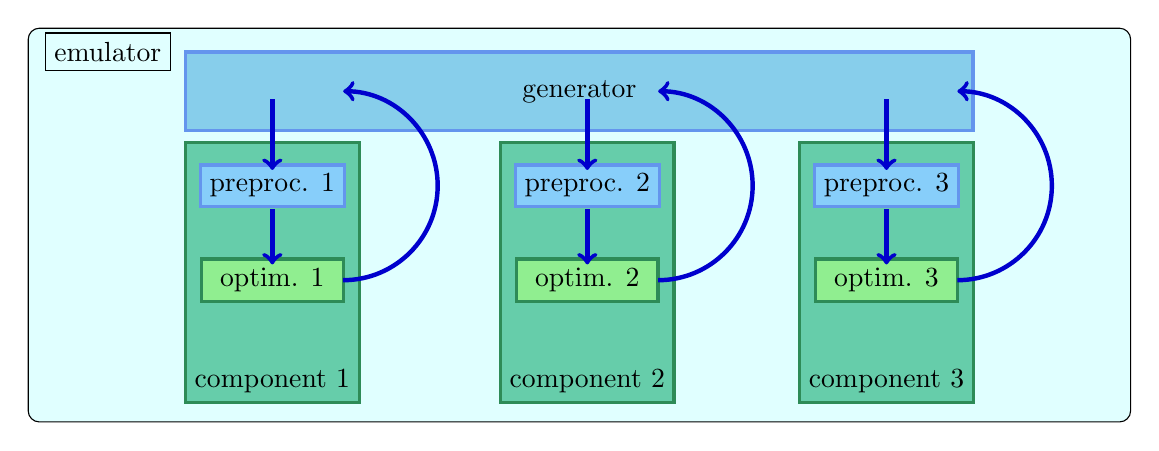
\begin{tikzpicture}[
    gennode/.style={rectangle, draw=CornflowerBlue, fill=SkyBlue, very thick, minimum height=10mm, minimum width=100mm},
    ppnode/.style={rectangle, draw=CornflowerBlue, fill=LightSkyBlue, very thick, minimum size=5mm},
    optnode/.style={rectangle, draw=SeaGreen, fill=LightGreen, very thick, minimum width=18mm},
    compnode/.style={rectangle, draw=SeaGreen, fill=MediumAquamarine, very thick, minimum height=30mm, minimum width=10mm, text height=30mm}, % red!60 e red!5
    ] % recupera nodi e frecce da overleaf tikz tutorial
      % \draw[rounded corners, black] (0, 0) rectangle (14, 5) node[pos=.1] {\texttt{emulator}}; % pos=.1: al 10% del viaggio da (0,0) a (14,5) aggiungi un nodo testuale
      % \node[draw, rounded corners, black] (0, 0) rectangle (14, 5) {}; % non gli piace
      \draw[rounded corners, black, fill=LightCyan] (0, 0) rectangle (14, 5) {};
      \node[draw] at (1.01, 4.7) {emulator}; % aggiungi il testo sopra direttamente^
      
      \node[gennode] (maintopic) at (7, 4.2) {generator}; % specificarne la posizione?
      
      \node[compnode] at (3.1, 1.9) {component 1};
      \node[ppnode] at (3.1, 3) {preproc. 1};
      \node[optnode] at (3.1, 1.8){optim. 1};
      \draw[ultra thick, ->, color=MediumBlue] (3.1, 4.1) -- (3.1, 3.2);
      \draw[ultra thick, ->, color=MediumBlue] (3.1, 2.7) -- (3.1, 2.0);
      \draw[ultra thick, ->, color=MediumBlue] (4, 1.8) arc (-90:90:1.2);
      
      \node[compnode] at (7.1, 1.9) {component 2};
      \node[ppnode] at (7.1, 3) {preproc. 2};
      \node[optnode] at (7.1, 1.8){optim. 2};
      \draw[ultra thick, ->, color=MediumBlue] (7.1, 4.1) -- (7.1, 3.2);
      \draw[ultra thick, ->, color=MediumBlue] (7.1, 2.7) -- (7.1, 2.0);
      \draw[ultra thick, ->, color=MediumBlue] (8, 1.8) arc (-90:90:1.2);

      \node[compnode] at (10.9, 1.9) {component 3};
      \node[ppnode] at (10.9, 3) {preproc. 3};
      \node[optnode] at (10.9, 1.8){optim. 3};
      \draw[ultra thick, ->, color=MediumBlue] (10.9, 4.1) -- (10.9, 3.2);
      \draw[ultra thick, ->, color=MediumBlue] (10.9, 2.7) -- (10.9, 2.0);
      \draw[ultra thick, ->, color=MediumBlue] (11.8, 1.8) arc (-90:90:1.2);
      
    \end{tikzpicture}
    \caption{Schematic representation of \textsc{CosmoLIME}.}
    \label{fig:cosmolime_schematics}
\end{figure}

Notice that in fig. \ref{fig:cosmolime_schematics} we have one generator, but several components. The reason for this is that codes like \texttt{camb} can generate multiple derived quantities (power spectra, predictions of observables, etc.) starting from the same set of parameter values, and we may want to train separate machine learning models on these different parts of the dataset; more on this later on. In general what we have is a generator that produces several streams of data in parallel, which are stored and fed sequentially to each component. The component currently in training takes the generated data, performs the preprocessing, then looks for the best model hyperparameters using the optimizer; if needed it will request more data and try again. The emulator class oversees this whole procedure.

\subsection{Common Design Rules}\label{subsec:common_design_rules}
To conclude this introduction to \textsc{CosmoLIME}'s technical explanation we describe a few mandatory design rules that are shared by all of \textsc{CosmoLIME}'s blocks.

\paragraph{Data Representation in Memory}
An important property of \textsc{CosmoLIME} is the \emph{shape of the data} it deals with. 
\textsc{CosmoLIME} performs functional regression to learn the mapping between cosmological parameters and power spectra; this means mapping a vector input (parameters) to a vector output (spectra predictions). We can therefore stack observations vertically, thus organizing our dataset into a pair of matrices i.e. rectangular arrays of real numbers. For this reason \textsc{CosmoLIME} represents the dataset in memory using mostly rectangular \texttt{numpy} arrays, which is a common choice for this type of problems.
Usually these arrays are small enough to comfortably fit into memory: dealing with tens of thousands of rows made of tens of real numbers is not an issue for modern computers; for this reason \textsc{CosmoLIME} always makes the assumption that a ``big data'' approach (i.e. offloading the matrices to disk and only load in memory a fraction at a time) is not necessary.\footnote{A big data approach is not impossible, just not implemented in the current version of \textsc{CosmoLIME} as it has not yet been deemed necessary.}
In general going forward we keep in mind that \emph{\textsc{CosmoLIME} datasets are rectangular arrays of real numbers}, i.e. matrices where the rows represent the observations and the columns the different variables.

\paragraph{Block independence}
As explained above \textsc{CosmoLIME} consists of several blocks, all of which work in tandem to assemble an emulator using an automated, standardized algorithm; the automated algorithm to assemble an emulator is the intended use-case of \textsc{CosmoLIME}. 
In order to ensure that different usages are also possible each block is designed to be not just collaborative with the others, but also fully independent; this means that each block can be manually instantiated, accessed, and used, while also being capable of working in harmony with the others. This is useful for testing purposes, but can also be relevant if we want to disassemble the main class after training (for example we may want to use the same trained preprocessing block to perform different analyses, which means we may want to be able to discard the generator and model attached to that block).
These two scenarios (blocks used on their own or together) are both allowed as long as we ensure that the classes are both human-friendly and computer-friendly, so that both a human and \textsc{CosmoLIME}'s automated procedures can easily use them; to achieve this there are both ``manual'' and ``automatic'' modes to use the methods in each class. This basically means that we can use the available methods interactively, i.e. by manually modifying the class' internal state as needed, or automatically, i.e. by fixing all the relevant arguments once and for all during object initialization, then calling its method with no arguments. This second approach is taken by the manager classes: they automatically instantiate the needed classes with fixed internal parameters and then use them always in the same way; a human instead can take them apart, use their methods with new values for the internal parameters, and so on.

\paragraph{Support For External \texttt{python} Data Science Packages}
\texttt{python} offers many great packages to extend its data analysis and machine learning capabilities; examples include \texttt{numpy}, \texttt{scikit-learn}, \texttt{pytorch}, and so on. In order to exploit these remarkable packages \textsc{CosmoLIME} has been designed with this in mind, using the ``open slot'' approach to ensure inter-package compatibility. For example the \texttt{optimizer} class is able to accept an arbitrary user-provided model; as long as the associated class contains a \texttt{.train()} method it can be used by \texttt{optimizer}, because its internal algorithm leaves an ``open slot'' to be filled with any class, then calls this object's train method. This level of abstraction (which consists of writing code where some elements are left as generic as possible and are then filled by the user) is shared by all software blocks; in this way all the great available packages can be used with minimal effort, requiring at most a wrapper to satisfy \textsc{CosmoLIME}'s consistency requirements. Were this not the case we would need to reinvent the wheel too many times, because we would need e.g. to re-implement common machine learning algorithms from scratch.

\paragraph{}
Finally we can now dive into the detailed explanation of exactly how these pieces work and communicate.


\section{Generator}
% importante il discorso che possiamo avere dati infiniti (potenzialmente), ergo non c'è solo da usare modelli più sofisticati (compromessi eccetera)

% ha senso mettere anche i dettagli tecnici del codice, ad esempio che possiamo scegliere un numero iniziale di samples da generare così come quanti aggiungerne ad ogni giro.

% Importante il discorso di alternanza fra generazione e miglioramento modello (parametro di ogni quante epoche generare) così come quello del caching delle componenti non attualmente in uso; tutto questo da illustrare con gli esempi di camb

% prova a vedere che succede usando meno dati, ad esempio se cosmolime decide di prenderne altri (non c'è bisogno di rieseguire la funzione, basta definire un sampling che sia un indexing statico del numero di righe richieste dove l'offset è dato dal seed*num iniziale, così scorro senza ripetizioni)

\subsection{Simulating Data}\label{subsec:simulating_data}
The most important part of any machine learning application is the dataset; without good enough and plentiful enough data the world's most sophisticated algorithm will still perform badly.\footnote{Many people in the machine learning community underestimate how often the same algorithm performs much better after new data is acquired or e.g. a better preprocessing pipeline is employed; this ``gamification'' of machine learning means that often people scramble to achieve the best score over some fixed dataset by changing the algorithm instead of acting upon the dataset itself.} An interesting aspect of \textsc{CosmoLIME} is related to this crucial point, as its treatment of data samples is quite unusual.

In most machine learning application the data is fixed, which means that the acquisition of new samples is not possible. For example many popular big data models require the assembling of huge datasets, which is an expensive and time-consuming procedure; therefore once the dataset has been obtained people would rather optimize the performance of the model rather than invest more time and money in the sampling of new data points.
Another common occurrence is that of noisy data; for example if the points in the dataset have been obtained by experimentally measuring some quantity (like e.g. in many scientific machine learning applications) then there always are spurious contributions of some sort afflicting the dataset. For this reason even in basic regression problems one always models the process as the sum of two contributions: a deterministic part (the actual model we care about) and a stochastic part (the noise term we would like to eliminate but cannot). Even though statistics can help deal with the ever-present noise (via preprocessing or noise modelling) it can never be completely removed.

Probably the most interesting feature of emulating cosmological power spectra from a machine learning perspective is that these two common limitations (fixed, noisy datasets) do not apply; to see why this is true let us compare the generic regression problem in machine learning with the one pertaining to \textsc{CosmoLIME}.
The typical situation where one applies regression is when an \emph{unknown} function must be learned from data; due to the fact that the mapping is unknown we can only measure $(x, f(x))$ pairs and use them to infer the overall shape of $f$. Furthermore if the $(x, f(x))$ pairs are obtained with an imperfect procedure (e.g. noisy measurements, suboptimal sampling) their quality constrains how accurately we can approximate $f$ with its $\hat{f}$ representation.
But when dealing with power spectra the mapping $f$ is \emph{known}; the point of emulation is to accelerate the evaluation of a known function, not learning an unknown one - therefore since $f$ is known it becomes possible to select an arbitrary set of points $\{x_n\}$ and evaluate the corresponding function values $\{f(x_n)\}$. This procedure has two important implications: in this machine learning problem we can generate as much data as we want, and the obtained samples will have perfect accuracy,\footnote{At least in principle; since $f$ is usually a complex function what is typically done is to evaluate it using numerical techniques, which may lead to inaccuracies.} since no noise sources are present.

Indeed notice that access to data with arbitrary quality and of arbitrary number is in general the main difference between the emulation task and a generic regression problem; the remaining elements (e.g. the numerical techniques) are instead shared between these tasks. This crucial difference hinges on whether $f$ is known (and just to be accelerated), as in the specific task of function emulation, or whether $f$ is unknown (and therefore to be actually discovered, at least approximately), as in the most general regression problem.

To recap: instead of approximating the relation between two fixed, noisy datasets we can generate as much noise-free data pairs as needed. Therefore when designing \textsc{CosmoLIME} we do not want a class that accepts a prebuilt dataset and passes it to the next layer; what we want instead is to implement a block capable of automatically sampling data points. This block's user provided input, therefore, is not a fixed dataset, but rather a \texttt{python} function capable of computing $f(x)$ when fed with $x$. 

These considerations steer the design process towards defining the \texttt{generator} block so that it performs the following actions:
\begin{enumerate}
    \item It generates new data samples when asked;
    \item It passes the obtained datasets to the appropriate parts of the emulator;
    \item Finally it optionally caches data, either in memory or on disk. Saving on disk is useful to avoid having to start from scratch in the event that unexpected errors cause the program to suddenly fail; saving in memory is needed to comply with the ``parallel generation, sequential training'' approach when dealing with multi-component datasets (see next sections).
\end{enumerate}
Let us discuss these points in more detail.

\subsection{Sampling Strategies}\label{subsec:sampling_strategies}
% griglia deterministica, prendere parametri a caso, non ci esprimiamo perché qui l'utente ha modo di sfruttare eventuali prior suoi (nel senso di problem knowledge ma anche letteralmente riguardo come campionare parametri)
As said above in the case of \textsc{CosmoLIME} the user can afford the luxury of not having to supervise the process of obtaining the dataset; instead they can simply give \textsc{CosmoLIME} the means to automatically assemble the dataset as needed. When discussing the \texttt{component} class below we will describe the logic used by \textsc{CosmoLIME} to decide more data are needed; for now we simply need to understand how \texttt{generator} can satisfy the request of simulating new points, when asked. To describe how this is implemented in \textsc{CosmoLIME} it pays off to approach the problem from a more general point of view.

Let us suppose we need to sample a function $f$ by evaluating it in some arbitrarily chosen points $\{x_n\}$, so that an output dataset $\{f(x_n)\}$ can be obtained. We want to use the $\{(x_n, f(x_n))\}$ pairs to learn an approximation of $f$, which naturally leads to the following question: how should the points $x_i$ be chosen to ensure the most accurate learned representation of $f$ possible? If we could sample infinitely many points we could achieve perfect approximation accuracy, but clearly this is impossible; ideally we want to choose the $x_n$ in strategic regions of parameter space, so that a good machine learning algorithm may be able to interpolate the missing parts of $f$ accurately enough.

Several strategies are possible to sample the $x_i$ points:
\paragraph{Grid Sampling}
The simplest possible approach is to define a grid of linearly spaced points, and use it to define the $\{(x_n)\}$ sequence. In the case of parameters with bounded values (i.e. parameters only defined in a finite interval) this is trivial; in the case of parameters that can be arbitrarily small or large (or even just defined in very large intervals) we need to select a minimum and maximum values in order to construct this grid. For example in the case of a function mapping 1D spaces after defining $x_{\text{min}}$ and $x_{\text{max}}$ (either arbitrarily or due to the physics of the problem) and how many points to sample we can compute each element of the $\{x_n\}$ sequence as follows:
\begin{equation*}
    x_n = x_0 + n\Delta x = x_0+n\frac{x_{N-1}-x_0}{N-1} = x_\text{min} + n\frac{x_{\text{max}}-x_{\text{min}}}{N-1}, \ \ n\in [0, N-1]
\end{equation*}
from which it follows that in this notation $x_0 = x_{\text{min}}$ and $ x_{N-1} = x_{\text{max}}$.

This approach to choose the $\{x_n\}$ sequence reflects a lack of preference for any region in the $\mathcal{X}$ space (i.e. the vector space the $x_n$'s belong to). Picking this sampling strategy is reasonable when we want to express the belief that no $x$ values are more important than others, or when we lack knowledge about the function's behaviour in $\mathcal{X}$. In general this sampling strategy represents not committing to any spot in particular, treating them all equally; in Bayesian terms we may state that this strategy is equivalent to an \emph{uninformative prior}, i.e. we do not express information that would allow to give different weights to different regions of $\mathcal{X}$ space.

% svantaggio gaussiana
This approach is indeed useful when the user knows that all regions of $\mathcal{X}$ should be sampled uniformly and deterministically, or if they're unsure about the shape of $f$ and want to pick the ``safe'' option; and yet this approach can be inefficient. Imagine for example that the target function $f$ is almost constant in region $\mathcal{X}_1$, while quickly varying in region $\mathcal{X}_2$; a simple example of this is a Gaussian, that is almost zero outside the tails and quickly rises to its maximum value once we start walking towards the peak. Now in this case having an equal number of points in $\mathcal{X}_1$ and $\mathcal{X}_2$ is inefficient: too many points in $\mathcal{X}_1$ is a waste because few samples are needed to accurately summarize $f$'s behaviour here, while too few points in $\mathcal{X}_2$ may cause the model to fail in the task of accurately capturing the shape of the function (at most the model can learn a sort of local average, while missing the high frequency details contained in $f$). This potential issue can be mitigated by increasing $N$: with a huge number of points in the dataset each part of $\mathcal{X}$ is bound to be adequately represented. In practice, though, $N$ cannot be too large, as we often have a limited computational budget: computing each $f(x_n)$ can have a non-negligible cost, so that large enough values of $N$ can be impractical. For this reason it makes sense to explore other sampling strategies, in particular strategies that are intrinsically asymmetric in the sense that they prefer certain regions of $\mathcal{X}$ over the others.

\paragraph{Uniform Random Sampling}
% uniform distribution
Another possible sampling strategy consists in selecting the $x_n$ \emph{randomly} in $\mathcal{X}$, then computing the corresponding $f(x_n)$ values. This can be helpful because with limited values of $N$ can introduce some asymmetry in the sampling procedure. Considering the previous example, where the target function $f$ varies slowly in $\mathcal{X}_1$ and quickly in $\mathcal{X}_2$, sampling the $x_n$ points randomly makes it possible that more point will happen to be in $\mathcal{X}_2$ rather than in $\mathcal{X}_1$. 

To better appreciate this result imagine that the overall behaviour of this function $f$ is unknown - that is, we know how to compute $f(x)$ for any $x$ but we don't know e.g. how $f(x)$ varies with $x$, and so on. Let us also imagine that in this situation $N$ cannot be too large due to computational budget constraints, and that the grid approach results in a model of $f$ with unsatisfactory performance. Even if we do not know about $\mathcal{X}_1$ and $\mathcal{X}_2$ by switching to a random sampling approach with a bit of luck we may stumble upon the efficient asymmetric distribution of the $\{x_n\}$ sequence in $\mathcal{X}$ space.

Assuming we lack prior knowledge about $f$'s behaviour in different regions of $\mathcal{X}$ the most reasonable distribution to use is the \emph{uniform} one, as we have no way of committing to a preference for e.g. $\mathcal{X}_2$ over $\mathcal{X}_1$; but this sampling strategy can lead to inefficiencies, too. Indeed unless $N$ is quite small the observed distributions of points will quickly converge to the uniform one they're sampled from, i.e. the sampled sequence $\{x_n\}$ will become symmetric with respect to the different regions of $\mathcal{X}$. Since this convergence is relatively quick this means that even for $N$ values that are not particularly big we recover the previous grid-based case, i.e. a sequence of points that fails to implement the asymmetry needed to increase the efficiency under budget constraints.

In order to achieve the desired asymmetry we may therefore restrict ourselves to small values of $N$; in this case the population distribution can actually significantly differ from uniform, and therefore be asymmetric in $\mathcal{X}$. The problem with this approach is that by staying away from convergence we cannot predict much about the resulting distribution, which basically means that whether the output sequence is good or not is left to luck. Assuming we can try to sample the population of points several times this may not be an issue: even if the first attempt failed maybe after 10 the resulting distribution efficiently captures $f$. In this case we will have sampled $10N$ points instead of $N$; if $N$ is small enough that $10N$ is not too expensive but e.g. $10^5N$ would be needed to ensure success with grid sampling then this uniformly random strategy can be successful. Unless we are in this sweet spot, though, it makes sense to implement a truly asymmetric sampling strategy.

% uniform prior: democratico, ma nel limite riproduce quanto sopra nel senso che nel limite è troppo simmetrico. Inoltre si basa sulla fortuna

\paragraph{Nonuniform Prior Sampling}
% custom sampling distribution
If prior knowledge about $f$ is available how to design more efficient samplers becomes almost obvious. Sticking to the grid approach, for example, we can ditch the linearly spaced grid in favor of one that is finer in ``hotter'' regions (those with more ``activity'') and coarser in the ``cold'' ones.
Another possibility is to use random sampling from a \emph{non-uniform} distribution: as we saw switching to a stochastic sampling strategy makes it possible to achieve a good $\{x_n\}$ sequence with much fewer points, but whether this possibility is actually realized in practice is unpredictable and therefore requires some luck. We remark that it becomes possible to decrease the amount of luck if a nonuniform distribution is employed: indeed if we know that $\mathcal{X}_2$ requires more points than $\mathcal{X}_1$ we can design the sampling distribution in such a way that points from $\mathcal{X}_2$ are more likely, and so on. In this sense a nonuniform distribution introduces the needed asymmetry in the same way as the nonuniform grid, but as mentioned multiple time can potentially reach the results with less points (with the price to pay being that we cannot know beforehand whether the next run will actually be successful).

\subsubsection{The Problem of Specifying Prior Knowledge}\label{subsubsec:prior_knowledge_generator}
% coarse grid, slightly finer grid, until the points are numerous and packed close to each other (per riciclare il parametro seed nel caso deterministico)
% tre passaggi
The discussion in the previous section outlines an important fact: \emph{it is best to avoid fully automating the sampling procedure}. What we mean is that, since each sampling strategy has pros and cons, the most efficient way to decide where to evaluate e.g. a power spectrum depends on the specific problem at hand, and on how the user decides to deal with it. For this reason we believe that the decision of the sampling strategy is best left to the user; not only that, but the user must also write a wrapper to their Boltzmann codes of choice. 

The \texttt{generator} class therefore expects a \texttt{python} function from the user; this function must do the following:
\begin{enumerate}
    \item Accept a \texttt{size} and a \texttt{seed} argument;
    \item Sample \texttt{size} number of points $\{x_n\}$ using the sampling strategy of choice, using the \texttt{seed} parameter as seed;
    \item Compute and return the $\{f(x_n)\}$ sequence by feeding the each $x_n$ to the exact code of choice.
\end{enumerate}
% SCHEMATIC REPRESENTATION USING TIKZ? TUTTE QUESTE FIGURE MI POSSONO TORNARE UTILI PER LA PRESENTAZIONE E RENDEREBBERO LEGITTIMA LA PRESENZA DI UN INDICE DELLE FIGURE

Defining this function is the only nontrivial piece of user-written code required by \textsc{CosmoLIME}, as the rest simply consists of specifying some arguments like which model is to be optimized. Indeed by using a user-provided function defined with these rules the \texttt{generator} can generate as many points as requested by \texttt{component}; the \texttt{seed} parameter can be used to ensure reproducibility and that the points sampled every time the \texttt{generator} is called are actually different.

\paragraph{What About Deterministic Sampling Strategies?}
Having \texttt{generator} rely on a \texttt{seed} parameter makes it seem that \textsc{CosmoLIME} is unfairly biased towards stochastic sampling strategies, but we the user can easily write the required function in such a way to comply with the \texttt{seed} argument requirements even assuming a deterministic sampling strategy. As we will see later \textsc{CosmoLIME} uses the \texttt{seed} parameter to increase the size of the training data in the event of unsatisfactory model performance by setting \texttt{seed} equal to the index of the current epoch. This means that the algorithm starts with a seed equal to 0, then if \texttt{component} determines that more data is needed it will ask \texttt{generator} to produce more using \texttt{seed = 1}, and so on; in the case of stochastic samplers this means sampling the distribution multiple times to collect more points. This means that the role of the \texttt{seed} parameters is simply controlling the size of the final dataset. Therefore if we write the above function with \texttt{seed} controlling the coarseness of the grid we can ensure that \textsc{CosmoLIME} will work as expected; for example with \texttt{seed = 0} the grid may be very coarse, while with \texttt{seed = 5} the grid is much finer. 
Due to this it seems that in the case of deterministic samplers the \texttt{size} and \texttt{seed} parameters overlap; after all if increasing the \texttt{seed} is supposed to produce a finer grid it must then imply a larger number of samples in the dataset, therefore overruling the number of samples to be generated specified by \texttt{size}. Furthermore this seems to be a problem, because a 10 times finer grid has 10 times as many points, resulting in the request of generating an ever-increasing number of points instead of the fixed value specified by \texttt{size}.

These issues are actually easily tackled in practice: since generating data is a cumulative process (i.e. the new samples are put in the same dataset as the old ones) we can create a finer grid by adding a fixed number of points, instead of starting from scratch with a larger number of points to produce. A possible way to achieve this with a fixed \texttt{size} and increasing \texttt{seed} is to generate linearly spaced grids offset by an amount depending on \texttt{seed}; in this way we can surely increase the density of points in our grid while at the same time keeping the number of generated points per epoch fixed.

We remark that other approaches are possible, and that we need not concern ourselves with details about the role of \texttt{size} and \texttt{seed}, as those will be explained later in more detail; the point of this paragraph is simply that the design philosophy behind \texttt{generator} is flexible enough to accomodate for arbitrary sampling procedures.

\subsection{Data Components: Parallel Generation, Sequential Training}\label{subsec:data_components_generator}
% mettere da parte gli altri dati: parallel generation, sequential training
Boltzmann solvers like \texttt{camb} \cite{camb} work by allowing the user to fix the detail of the cosmology (model, parameter values, etc.), then computing predictions for several observable quantities; we call these separate outputs \emph{components}. Dealing with multiple components is useful because by observing the corresponding quantities in independent experiments we have multiple ways of constraining the cosmology, considering their common source. For this reason it makes sense to have separate machine learning predictors, one for each component i.e. one to replace each separate theoretical prediction. 
An important property of softwares like \texttt{camb} is that predictions come in bulk: the software outputs \emph{all} of these components in a single batch; this has the advantage of allowing for \emph{parallel data generation}, in the sense that a single call to \texttt{camb} returns the input-output pair of values for all the observables at the same time. In theory this would allow \textsc{CosmoLIME} to also train the model associated to each component at the same time: as the new data arrive each part of them is streamed to the appropriate component, which then proceeds to train its respective model at the same time. The problem with this is that training a machine learning model can be quite intensive: depending on the complexity of the model all the available computer resources may be required. In order to avoid reaching obvious bottlenecks \textsc{CosmoLIME} was designed in such a way that data are generated in parallel, but the corresponding component models are trained in sequence; we will describe later how this works in practice.\footnote{As stated it is wiser to train one model at a time; hence what \textsc{CosmoLIME} does instead is to optionally use the approach discussed in the next sections to train several versions of the same model in parallel. Possible extensions of this ``partial parallelization'' will be discussed later on.}

For now we remark that this ``parallel data generation, sequential training'' approach means that \textsc{CosmoLIME} alternates between a data generation phase and a model training one, with the property that during the data generation all component datasets are sampled, while during the training one only one model at a time. In order to comply with this algorithm \texttt{generator} has a way to hold onto data that will be used later: every time it is requested to generate data for e.g. component 1 it generates data for \emph{all} components; then it returns the data for component 1 and stores the remaining component datasets in memory or on disk, to be used when the training phase switches to the other components' models. This \emph{component caching} functionality is a core part of \texttt{generator}; in particular its component data generation method simply wraps the method used to call the user-provided function with this separation and caching of components.

\subsection{Other \texttt{generator} Features}
% salvare su disco, accettare parametri... roba pallosa e più o meno intuibile da quanto sopra
The remaining arguments when initializing \texttt{generator} can be used to customize the saving behaviour; for example in the case of datasets that require expensive computations one can enable the saving or offloading of the other components' datasets to disk, and even though this slows down \textsc{CosmoLIME} it can prevent the need to face long waits multiple times in the case that the software suddenly stops due to an error. Other options can be used to set hyperparameters in the user-provided function, and to allow for the saving and loading of datasets in separate locations: if for example a dataset is already available (e.g. because the user has already simulated data with the same function) it can be loaded and used as a starting point, so that \textsc{CosmoLIME} does not have to generate data completely from scratch. There are also options to avoid overwiting this ``prior'' dataset, so that previous analyses can be kept separate.

Finally notice that by default datasets are saved to or loaded from disk using either the \texttt{.npy}, \texttt{.npz} or compressed \texttt{.npz} format. As stated above we are performing regression, which means that our datasets are comprised simply of matrices: for example the input is a matrix whose rows represent different ``observations'' (i.e. different values for the set of input cosmological parameters), while the columns represent different parameters altogether. Since we are dealing with ``rectangular'' datasets of real number these datasets are efficiently represented as \texttt{numpy} arrays; we therefore also save them to disk using \texttt{numpy}'s methods.


\section{Preprocessing}
\begin{comment}
- i tecnicismi tipo nan remover e constant features remover?
- log: riduci il dynamic range tipo cosmopower quando possibile (features positive), ma almeno in output a volte ha senso anche analiticamente (ad es. il log di una MVN è solo la parte di forma quadratica) - direi che questo è più un esempio per contestualizzare il log, qua si parla di preprocessing, schiacciare gli ordini di grandezza mi sembra più pertinente
- media a zero e varianza a 1, utile ad es con le NN ma non con gli alberi. In alternativa: min e max a 0 e 1, eccetera
- whitening: media a zero e covarianza identica (cioè identità non solo sulla diagonale ma ovunque, tolgo le correlazioni fra variabili, cioè tengo solo le dipendenze statistiche di ordine superiore)
- super whitening: cross correlation fra input e output, rendo identica la cross correlation (una specie di super covarianza) fra input e output. In questo modo considero una dipendenza statistica "semplificata", che tenga solo gli ordini superiori. Questo viene fatto con la procedura del prof. Chiarire sia perché questa procedura funzioni sia più in generale a che serva.
- altro? Rivedi il codice
- (prima) discussione generale di trasformazioni solo di input o output, o quelle accoppiate, congiunte
\end{comment}
\subsection{Standardized Preprocessing Interface}
The most important part of any machine learning application is the dataset; the second one is the preprocessing, and the last one is the model. The reason for this is that if the training data's quality is poor not even the world's most advanced model can turn those samples into accurate predictions. Having covered how we can generate and manage an arbitrary number of arbitrarily accurate samples we now turn to the problem of designing a standardized interface for arbitrary data preprocessing transformations.
% differenza con dataset: anche se resta possible avere trasformazioni completamente fatte dall'utente stavolta possiamo offrire trasformazioni di default ragionevoli, in quanto trasformazioni universali sicuramente esistono - a differenza di "dati universali", che non esistono in quanto evidentemente dipendenti dal problema in questione.
The problem of choosing a (set of) preprocessing transformer(s) is similar to that of choosing the data generation/sampling procedure, in the sense that the user should decide one of several possible approaches depending on the problem at hand. As we saw we can interpret the choice of the generation algorithm as reflecting some sort of prior knowledge on the problem; the same is true for data preprocessing, because data preprocessing transformations must be chosen according to the special characteristics of the problem and of the model of choice.
In the case of \texttt{generator} this is a necessity: there is no universal way to generate data because they clearly depend on the physics of the relevant situation; and yet this is no longer true in the case of preprocessing. Indeed there exist ``universal'' transformations of the data, in the sense that some transformations that are useful in a large class of problems (for example standardizing the dataset's mean and variance can help numerically stabilize a neural network's training); for this reason \texttt{preprocessing} can be asked to implement one of \textsc{CosmoLIME}'s default transformers (do note that custom made transformers can still be used, of course).

The \texttt{preprocessing} class in \textsc{CosmoLIME} works in a similar way as \texttt{generator}: the user provides either a custom or default (set of) transformer(s), then \texttt{preprocessing} fits its hyperparameters to the data (if any; see below). Once this is done \texttt{preprocessing} can be used as any other \texttt{python} function, i.e. it can take any pair of input/output datasets and return the transformed versions. Notice that if an inverse transformation is available a method computing it is contained in the corresponding class, too; not all of them have it because some transformations discard informations and are therefore irreversible.
% FIGURA SCHEMATICA IN TIKZ?

\paragraph{Joint Transformations}
Most preprocessing transformations are applied to only the input or the output matrix; for example as we will see below in order to ensure that the input dataset's features have zero mean it suffices to subtract their averages, without the need to involve the output dataset.

Some transformations, though, are \emph{joint}: they involve both the input and the output dataset (for example \texttt{NaNJointRemover}; see below). For this reason the \texttt{preprocessing} module has internal subclasses that correctly interface with any transformation depending on whether it is joint or not. Therefore two informations must be specified by the user should they want to provide a custom transformer: the mathematical transformation and whether or not \texttt{preprocessing} should consider it a joint input/output transformation.

\subsection{Default Transformers}\label{subsec:default_transformers}
% listona in paragrafi?
% ConstantFeaturesRemover NaNJointRemover LogTransformer Log1pTransformer StandardScaler Whitening (vari schemi, cita paper pca, più complesso: joint decorrelation...)
Several prebuilt transformers are available in the \texttt{preprocessing} module for the user to choose from; let us review them. 
\subsubsection{Recommended Transformers}
\textsc{CosmoLIME}'s default option for preprocessing consists of the sequence of the following transformations.\footnote{Of course the default option is not mandatory: the user can choose a different set of transformations, or even disable preprocessing entirely.}

\paragraph{\texttt{NaNJointRemover} Transformer}
A typical use-case of \textsc{CosmoLIME} consists in generating data using \texttt{camb}. This means that the generator will pass a set of cosmological parameters values to \texttt{camb}, which will respond with the theoretical prediction of some observable conditioned on those values for the cosmological parameters. For technical reasons certain input values lead to outputs containing \texttt{NaN} (not a number) values; of course it usually is impossible to know beforehand which numerical values ``corrupt'' the predictions, and we can only compute predictions and a posterior ban the inputs that led to the empty outputs.

Some machine learning algorithms and preprocessing transformations are capable of dealing with \texttt{NaN} inputs, either by ignoring them or by classifying them separately (e.g. some decision trees-based models can do this distinction); but considering that the vast majority of machine learning models will fail if \texttt{NaN}s are not removed it is wiser to discard them from the dataset. This is an example of a joint transformer: we want to remove rows from the input matrix depending on the output one.
The \texttt{NaNJointRemover} transformer solves this problem by obtaining a logical mask which marks which rows in the output matrix contain at least one \texttt{NaN}; this mask is then used to drop the coupled rows from both matrices, i.e. the rows in both matrices which share the same index. 

For obvious reasons the logical mask used to flag and remove bad rows is recomputed every time a new dataset is presented.
We also remark that the discarded rows are not saved anywhere, therefore this transformation is irreversible, hence why it is given an identity inverse transform.

\paragraph{\texttt{ConstantFeaturesRemover} Transformer}
Sometimes the user-provided function passed to \texttt{generator} can have redundant outputs%. 
% For example when computing the predicted luminosity distances associated to a grid of redshift values the distance at $z=0$ will always be zero, by definition; since this value is the same irrespective of the employed cosmology one output feature (i.e. matrix column) will be constant and equal to zero. % non ne sono più così sicuro...
; for example the generation code may produce a constant feature i.e. a constant column; due to this all rows share one element, which means all but one are redundant.
The user can account for this by slightly tweaking their code, but in the event they forget about it or do not want to deal with this correction themselves it makes sense to check for constant features. 
The \texttt{ConstantFeaturesRemover} performs this automated check and correction; it does so by computing a logical mask to flag columns whose elements all share the same value. This is achieved in a vectorized fashion by assigning \texttt{True} to the columns (if any) whose elements are all equal to e.g. the first one. If the mask produced this way flags any column (either in the input or the output) those columns are removed from the respective matrix, similarly to the previous transformer. The main difference is that this transformation is invertible: this class remembers the index of the discarded column and its only value, so that it the original matrix may be easily restored. To achieve this two arrays (positions and values) are stored in the transformer.

\paragraph{\texttt{StandardScaler} Transformer}
As discussed in section \ref{subsec:nn} a simple preprocessing transformation that often results in improved performance (especially in the case of some models, like e.g. neural networks) is \emph{feature standardization}; standardizing the features means rescaling each variable i.e. each column according to one of several possible rules. For example a common choice consists in rescaling the variables so that they all have zero mean and unit variance. To achieve this it suffices to compute the mean and standard deviation along rows, i.e. the mean and std obtained using the elements of all the rows; we can then subtract the mean array from each row, then divide by the std array, resulting in a matrix whose rows have zero mean and unit variance.
Using numpy this is easily achieved using a vectorized approach: \texttt{(x - x.mean(axis = 0))/x.std(axis = 0)}.

This transformation is invertible, too: by remembering the mean and std arrays of the original dataset and inverting the algebric operation given above the original matrices can be reconstructed exactly. This in turn requires that this transformer, too, must hold an internal state, whose value is to be learned by fitting the data.

As a final remark we note that this transformer is not custom made, as are the other two; it actually comes with no modifications from the \texttt{scikit-learn} package. This is consistent with one of \textsc{CosmoLIME}'s design principles, namely support for external \texttt{python} packages; this is just one example of how beneficial the consequences of \textsc{CosmoLIME}'s design philosophy can be in practice.

\paragraph{Default Transformer}
The default preprocessing transformation consists of the previous three transformers, in the same order as above. The first two don't really have disadvantages and should always be utilized, as they basically check for imperfect or suboptimal \texttt{generator} outputs, that the user did not preemptively account for. The last one is a less obvious choice: even though feature standardization often helps or is innocuous at most (for example in the case of decision trees), experience tells that sometimes standardizing the features can actually impede convergence speed or accuracy, as it often is a nontrivial modification of the data distribution. In this cases or in the event the user is unsure the scaling transformation can be disabled easily enough; since the ``helpful or harmless'' cases are more common we decided to leave it in the default transformer anyway.

\subsubsection{Optional Transformers}
\textsc{CosmoLIME} currently includes other preprocessing transformations; since these do not always improve the training procedure they are left to the user's discretion. 
A few examples are reported here.
% log, log1p, whitening + io decorrelation
\paragraph{\texttt{LogTransformer}}
There are several situations where applying a logarithm to the input or output features can greatly aid an inference pipeline. For example since Gaussian likelihoods are very common in cosmology a standard procedure is to compute the \emph{log-likelihood} instead of the original likelihood; in this way it becomes possible to only deal with the quadratic form. This is exactly what softwares like \textsc{CosmoPower} do; instead of computing the power spectra directly they predict their \emph{logarithms}.

Applying a logarithm transform in situations like the previous example is a natural choice due to the mathematical properties of the problem at hands; even when there are no obvious reasons to do so using logarithms can be useful.
One of the oldest tricks of modern science is to use logarithms to \emph{reduce the dynamic range of variables varying in a large interval}; this simply means that logarithms perform a nonlinear compression of intervals, with the property that same-width intervals get more and more compressed as they cover larger and larger values. The effect of this procedure is that it redefines the scale of the variables is such a way that instead of having linearly spaced \emph{values} we have linearly spaced \emph{orders of magnitudes}. 
To understand why this can be useful imagine we have a variable $x$ defined in the $[0.1, 10^5]$ interval; in order to cover this interval a model like e.g. a neural network must contain weights with large numerical values, which means that the network becomes insensitive to small variation of $x$ - which is a natural consequence of the fact that e.g. variations of order unity are negligible when e.g. $x \sim 10^4$. If a change in $x$ from $0.1$ to $1$ is as physically relevant as the change from $10^4$ to $10^5$ this is a problem: due to the large size of the relevant interval a machine learning model is expected to lose resolution near the left extremum, i.e. it becomes insensitive to small variations.
Contrast this with the situation in which we analyze not $x$ but $\log_{10}x$; now the full interval is $[-1, 5]$, and the variations from $0.1$ to $1$ or from $10^4$ to $10^5$ become variations from $-1$ to $0$ and from $4$ to $5$, respectively. This makes it clear that using logarithms consecutive orders of magnitude become linearly spaced; in this particular example both increments become equal to one (in general of order unity) due to the fact that both consist of increasing from one order of magnitude to the next. For this reason log-transforming features helps the model gain the same sensitivity to variations of different orders of magnitudes - which as we saw is beneficial in situations where the dynamic range of a variable (i.e. the interval in which the variable is defined) is too large.

Another advantage is that logarithm can stabilize training of models like neural networks, as they can become numerically unstable if fed very large numbers. In our example applying the logarithm can compress the interval $[0.1, 10^5]$ (length equal to $10^5-0.1\approx 10^5$) to $[-1, 5]$ (length equal to 6), which no longer forces the network to deal with numbers much larger than of order unity. Up to numerical precision $x$ and $\log x$ hold exactly the same information since the logarithm is perfectly invertible, which means we can use logarithms to stabilize model training basically for free.

A final advantage in using the logarithm is that it can favorably modify what is optimized by minimizing the MSE loss; taking \textsc{CosmoPower} as an example we can state that `` taking the logarithm of the spectra reduces the dynamic range in the training data, and ensures that minimising the mean-square-error loss optimises for fractional (rather than absolute) accuracy on the emulated power spectrum. [Furthermore] standardisation ensures more rapid training convergence'' \cite{cosmopower}. As just stated their preprocessing mainly consists of taking the log of the output variables, then standardizing them to zero mean and unit variance.

Their last statement brings us to our final point: should we choose to use a log-transform it is mandatory to standardize \emph{after} the logarithm, \emph{not before}. Indeed if we standardize before and then apply the logarithm the results will surely have a mean different from zero and a variance different from one, as we just performed a nonlinear compression of the variables. Therefore the correct approach is the standardization of the logarithmic features, not the other way around.
Considering that this data transformation is optional\footnote{One may argue that if the logarithm transform offers so many advantages it should be included by default; a simple counterargument to this point is that the logarithm is only defined for positive values, so in the presence of negative values applying logarithms is forbidden. Technically it is possible to simply shift the features by adding a value large enough to make them positive, which is easy to do; and yet as this may have nontrivial consequences regarding the variables' distributions (especially after a scale-sensitive transformation like the logarithm) we prefer to avoid approaches like these.} it must manually be added; the above point means that we cannot simply append it to the default one, but rather should prepend it to the \texttt{StandardScaler}.

\paragraph{\texttt{Log1pTransformer}}
This class implements the transformation $x' = \log(1+x)$. Due to its similarity with the previous one it shares the same advantages; this is especially true for large $x$ values, as they satisfy the condition that $x+1\approx x$. The crucial difference between the two becomes apparent in the small-$x$ regime, as we can show as follows.

We know that for large $x$ values the logarithm varies slowly. This property can be made more quantitative by recalling the property that $\log_a a^b = b$; from this property it follows for example that $\log_{10} 10^4 = 4$ and $\log_{10} 10^5 = 5$ which basically means that \emph{to increase by one the logarithm's output we must increase by one the order of magnitude of its input}. Notice that this is exactly the nonlinear, orders of magnitude-based compression property of the logarithm we took advantage of above. 
The same property when $x<1$ causes the logarithm to vary exponentially quickly, instead. For example if we go from $0.1$ to $0.01$ $\log_{10}x$ decreases from $-1$ to $-2$; if instead we go from $0.01$ to $0.001$ the logarithm goes from $-2$ to $-3$, and so on. Notice that the absolute-value difference between the first pairs of values is 10 times as large as the second (an order of magnitude less, as expected); this means that when $x<1$ the logarithm amplifies tiny argument variations more and more as the argument gets closer and closer to $0$. This causes the logarithm to quickly diverge to $-\infty$ as $x\to 0^+$.

Imagine therefore we are trying to analyze the variation of some variable $x$ that is strictly positive but close to zero at its minimum value; the logarithm amplifies tiny variations if they are close to $0$, which means that the logarithm is exponentially too sensitive in this scenario. If we shift $x$ by $1$ this problem is solved: since $\log(1+x)\sim x$ for $x\sim 0$ tiny variations in $x$ when $0<x\ll 1$ produce variations in the logarithm of the same scale, thanks to this approximately linear behaviour.
For large $x$ values adding $1$ does not produce significant changes in the logarithm; therefore this new transformer is advantageous when $x$ is defined over a large dynamic range, with its minimum very close to $0$ and in a scenario where variations in the left side of this interval are critical.

If $x_{\text{min}}$ is of order unity (i.e. not much smaller than $1$) it's best to avoid using the shifted logarithm, as a linear transformation of the input becomes nonlinear after the logarithm's application, which can have unpredictable effects on the data distribution; for this reason the standard logarithm transform should always be preferred when possible.

\paragraph{\texttt{WhiteningTransformer}}
We saw before that standardizing the mean and variance of input features can accelerate and/or stabilize the training of e.g. a neural network. A basic standardization is simply a linear rescaling of the features, which therefore simply normalizes the range of possible values. A more substantial transformation consists of also \emph{decorrelating the input variables}; this means that instead of just setting the diagonal of their covariance matrix equal to a vector of ones we \emph{turn the covariance into the identity matrix}. Decorrelating the input variables means that their are independent at first order; the only remaining statistical dependences are of second order or higher. Depending on the problem at hand this may simplify the analysis, as the data distribution becomes ``lighter''. This decorrelation can be achieved using linear operations; interestingly the solution is not unique, i.e. there are multiple algorithms that achieve the same identity covariance matrix - for example there are algorithms based on PCA or on the Cholesky decomposition. These solutions differ in some metric; for example one ensures that the transformed variables are as similar as possible to the original ones according to some similarity measure, while another maximizes the shared information between original and transformed variables. A great review of these results can be found in \cite{whitening}.

A similar transformation can be extended to the joint case; namely we can turn into the identity the \emph{cross-correlation between input and output variables}, which means removing correlations not just between different input variables but between input and output ones.

These transformations are implemented in the \texttt{WhiteningTransformer} class.


\subsection{Other \texttt{preprocessing} Features}
% prof Raveri: voglio poter salvare il preprocessing transformer, buttare i dati in mio possesso e rifare predizioni su dati nuovi - il che mi richiede di salvare il preprocessing. Discorso di pkl vs npy o npz?
The \texttt{preprocessing} module offers tools to save the instances of the generated classes to disk, similarly to \texttt{generator}. In that case the rationale was that we wanted to save the simulated dataset, either to use them separately in other analyses or to recycle them in future \textsc{CosmoLIME} runs; now the idea is that we may want to use the instances of preprocessing transformers separately. For example once the final emulator is deployed the training dataset must be left behind, i.e. the emulator must be able to output predictions to arbitrary inputs as requested by the inference pipeline. If the e.g. neural network inside the emulator has been trained e.g. on standardized logarithmic features, though, we cannot use the given input directly; we must first pass it through the preprocessing transformer, which is why \texttt{preprocessing} classes must have a ``save to disk'' functionality and be able to work independently.
This realistic example is one of the scenarios that motivated the independence design principle described in sec. \ref{subsec:common_design_rules}.

The other main difference between \texttt{generator}'s and \texttt{preprocessing}'s saving functionality is the format used; namely, the former uses \texttt{numpy}-based formats (\texttt{.npy} or \texttt{.npz}), while the latter relies on \texttt{python}'s \texttt{pickle} library (therefore on the \texttt{.pkl} format). The reason for this difference is that preprocessing transformers vary quite a bit. We know the information contained in \texttt{generator} worthy of being saved to disk is the dataset, which as stated many times is comprised of a pair of arrays; therefore it makes sense to use \texttt{numpy} formats.
The same is true for some preprocessing transformers; for example \texttt{ConstantFeaturesRemover} also relies only on a pair of arrays to define its internal state. Other transformers, such as \texttt{LogTransformers}, implement a mathematical transformation that depends on no external parameter, and therefore does not need to be saved at all.
The issue arises when we consider for example \texttt{StandardScaler}: even though its internal state too consists of a pair of arrays these are not easily accessible, as this class was taken with no modifications from \texttt{scikit-learn} and the original does not support accessing its internal state; therefore even if in principle \texttt{numpy} formats could still be used in practice this requires the annoying task of reinventing the wheel. Another issue is that other transformations may depend on things different from arrays; therefore whether or not \texttt{numpy} formats can be used depends on the transformer itself, and is not always true.

Instead of dealing with the different behaviours of these classes by e.g. trying to dig and standardize their internal states we choose the lazy approach of using \texttt{pickle}. This package can create a binary representation of arbitrary \texttt{python objects}, therefore making it easy to restore any variable in a new \texttt{python} session. Of course the \texttt{.pkl} is less efficient than \texttt{.npy}, given it must support more general scenarios; but for our purposes this difference is irrelevant, so we stick with our decision.

\section{Optimizer}
% se il punto fosse addestrare un modello senza iperparametri non ci sarebbe bisogno di automatizzare così il tutto: basterebbe generare un botto di dati e fare il training. Il problema è che se si usa una rete neurale anziché una regressione lineare questi iperparametri sono tanti e problematici, e per questo per risparmiare il tempo dell'utente anziché costringerlo a testarli da sé gli permettiamo di fornire dei range entro i quali campionare possibili valori degli iperparametri, poi l'optimizer se li sa scegliere da solo.

% parla di optuna! Modifica: wrapper con interfaccia funzionale, api funzionale, cioè che descriva cosa si vuole fatto anziché nello stile imperativo di base di optuna

% optuna other features: easy paralleliz, logging, saving benchmark dataframe to disk
\subsection{Model Hyperparameters Optimization With \texttt{optuna}}
Having understood how to deal with the most important parts of any machine learning application (the dataset and the preprocessing) we turn to the third most important aspect: \emph{model optimization}. In order to deal with this critical matter \textsc{CosmoLIME} provides the \texttt{optimizer} class, which implements the logic needed to efficiently implement hyperparameter optimization. To gain understanding about how this happens in practice let us discuss a few simple examples.

Imagine that the mapping we are trying to learn is simple enough that simple linear regression suffices to accurately model it. This model has no hyperparameters: given a training dataset the coefficients of the linear predictor can be computed analytically with no need for external hyperparameters. In this case there is no need to automate the implementation of the emulator, as it suffices to generate a large dataset and use it to train a single model.
The problem is that models with no hyperparameters such as linear regression are not \emph{expressive} enough, which means they fail to accurately model complex relations between data. More powerful model are necessarily more complex; in particular this extra complexity also implies an increased number of hyperparameters. 
An obvious example of this is your average neural network, whose final performance strongly depends on many potentially problematic hyperparameters, such as the network shape (number and lengths of neuron layers) and regularization type/strength. In general it is impossible to predict which hyperparameter values will generate the best model performance, and the only real solution of this problem is to pick many possible hyperparameters values, try the model using them, then choose the best performing one.
A common approach to understand which hyperparameters values lead to better model performance is using a \emph{validation set}. The idea is that instead of just splitting the original dataset into training and test set we reserve some samples for a third set, called the \emph{validation set}; by testing the model's performance on the validation set we can assign a statistically accurate score to any particular set of hyperparameters values \cite{understanding_ml}. Both the test and validation sets are not used to train the model; the difference is that the test set is used to assign a score to the final model \emph{after} hyperparameter optimization has been definitely completed, while the validation set is used to assign scores to different hyperparameter values \emph{during} optimization.\footnote{There are statistical reasons why the two sets must be kept separate even though they have a similar purpose - namely that if we modify the model after seeing the test score the test set becomes part of the validation set, and we can no longer use it as a reliable estimate of the true error. See for example \cite{understanding_ml} \cite{ml_probabilistic_perspective}.}

The standard machine learning approach to hyperparameter optimization is therefore as follows:
\begin{enumerate}
    \item Pick several values for the hyperparameters, \emph{according to some sampling procedure};
    \item Train the model on the training dataset, then use the validation error to assign a score to each hyperparameter value;
    \item Choose the hyperparameters with the best scores.
\end{enumerate}

The only remaining problem to solve is therefore how to choose the hyperparameters values we want to compare; interestingly enough \emph{this issue is entirely analogous to the one discussed in section \ref{subsec:sampling_strategies}}. Indeed if we opt for a grid-search approach we can in principle exhaust hyperparameter space, but in order to do so the grid must be fine enough, which in practice means that the required number of samples (and therefore the number of times a potentially complex model must be trained) needed to achieve the desired accuracy may be too large to be practical.
Once again switching to random sampling may be more efficient (as long as we happen to stumble upon a good solution, which requires an unpredictable number of attempts); just like in section \ref{subsec:sampling_strategies} we face the issue that the only ``universal'' choice of the sampling distribution, i.e. the uniform one, can be plagued by the same inefficiency issues as the deterministic grid search approach.
In section \ref{subsec:sampling_strategies} we argued that this issue can be solved by using prior knowledge to define a distribution whose shape (approximately) maps the ``hot'' and ``cold'' spots; the idea is that if a certain region contains more interesting samples (assuming some definition of ``interesting'') by increasing the probabilities associated with that region we can ensure our sampler will actually spend more time there - which is what we want.
In that case such prior knowledge is readily available, at least in principle; exploiting the fact that the target function is known one can easily get at least an idea about which regions are more valuable, either using the function's physical/mathematical properties or by manually inspecting it using \emph{exploratory data analysis} (EDA) techniques.
This approach is clearly impossible here: in this case the optimization target is the loss as a function of hyperparameter values, which means that there are no direct numerical algorithms to understand the shape of the function. Also this function can be quite complex, given how large the number of hyperparameters can get.

It is then clear that unfortunately this time there is little hope of obtaining a prior distribution from which to sample hyperparameters value in an efficient way; it seems the only realistic prior is an inefficient uniform distribution. But what about a \emph{posterior} distribution?
In general we would like to obtain a distribution over hyperparameter values whose probabilities are inversely proportional to the model's error when trained using those parameters: an efficient hyperparameter optimization should spend more time where the resulting loss is lowest. Actually using Bayes' theorem \emph{such a distribution can be constructed on the go}; the idea is conceptually simple. In particular even if we start from a uniform prior (i.e. we sample points from hyperparameter space with equal probabilities) after having obtained some data (i.e. trained the model a few times, using the sampled hyperparameter values) some regions will appear better, in the sense that points sampled there lead to lower errors. Therefore the observed data compels us to update the distribution's probabilities: points should be sampled more often in the low-error regions, which evidently are actually high density regions of this inverse-loss distribution in hyperparameter space. This procedure is exactly the content of Bayes' theorem, which is the idea that \emph{observed data should update the credibility assigned to different hypotheses}.

Luckily for \textsc{CosmoLIME} there exists a very advanced, easy-to-use and open source software frameworks that implements this \emph{Bayesian hyperparameter optimization}, called \texttt{optuna}. \cite{optuna}
\texttt{optuna} samples points from a prior in hyperparameter space, uses them to train the provided model, then uses the resulting validation errors to update the prior and assemble a posterior in hyperparameter space. This distribution then becomes the new prior, which ensures that future points are mostly sampled in the low-loss regions, and so on. Using this Bayesian approach \texttt{optuna} is therefore capable of computing accurate posterior distributions in hyperparameter space, and the more \texttt{optuna} runs the less time is wasted in high-error region losses. How all of this actually happens in practice is quite complicated, due to the fact that \texttt{optuna} uses very advanced sampling algorithms to efficiently and quickly ensure posterior convergence; a detailed discussion of these topics is beyond the scope of the present work, but can be found in \cite{optuna} and on \texttt{optuna}'s website.
For our purposes it suffices to state that using uniform random hyperparameter sampling is like blindly walking around hyperparameter space, just \emph{hoping} to find good values by chance alone, whereas using \texttt{optuna} is like having a compass that tells us which direction maximizes the probability to reach the objective. In particular this imaginary explorer starts with just a compass, but by using it they can write down a map of the area, and over time refine this map as more places are explored; after some time the map is accurate enough that the explorer can be confident enough in where the hidden treasure is located.

\texttt{optuna} represents the perfect solution to the problem of efficiently optimizing hyperpameters, as the Bayesian approach described above really is the current state of the art in the field of hyperparameter optimization. Other nice features that \textsc{CosmoLIME} inherits include:
\begin{itemize}
    \item \texttt{optuna}'s easy parallelization options (i.e. with a trivial code modification it becomes possible to test multiple hyperparameters at the same time, by training the corresponding models at the same time);
    \item Extensive logging tools;
    \item Support for streaming model benchmark data to disk using a simple SQLite database;
    \item ...and many more.
\end{itemize}
Due to all these reasons there is no doubt that \texttt{optuna} is a powerful tool to tackle any machine learning problem - and \textsc{CosmoLIME} is no exception. What remains to discuss is therefore a possible way of wrapping \texttt{optuna}, with the aim of turning into a piece of \textsc{CosmoLIME}; in particular this requires modifying the way \texttt{optuna} accepts user input.

% optuna other features: easy paralleliz, logging, saving benchmark dataframe to disk
\subsection{Wrapping \texttt{optuna} With A Declarative Interface}
% discorso di API imperativa o funzionale
% parla di optuna! Modifica: wrapper con interfaccia funzionale, api funzionale, cioè che descriva cosa si vuole fatto anziché nello stile imperativo di base di optuna
\subsubsection{Standard \texttt{optuna} Usage}
Due to how \texttt{optuna}'s API\footnote{An \emph{application programming interface} (API) is a way for two or more computer programs to communicate with each other. It is a type of software interface, offering a service to other pieces of software. A document or standard that describes how to build or use such a connection or interface is called an API specification. A computer system that meets this standard is said to implement or expose an API. The term API may refer either to the specification or to the implementation. In particular in this section we refer to \texttt{optuna}'s API to speak about the specific form \texttt{python} code must be written in in order to access \texttt{optuna}'s functionality.} works some modifications are needed in order to turn it into a potential \textsc{CosmoLIME} block; to see why let us briefly review how \texttt{optuna} is used in practice.

In order to train a machine learning regression model \emph{without} hyperparameter optimization it suffices to write a code that performs three steps:
\begin{enumerate}
    \item Read the data;
    \item Define and train a model;
    \item Test the model.
\end{enumerate}
Assuming a code performing the above operations has been written thanks to \texttt{optuna} it becomes possible to add hyperparameter optimization with trivial modifications. In particular the user is required to wrap the previous code to define an \texttt{objective} function, inside which the numerical values for the hyperparameters are replaced with placeholders that will be ``suggested'' (i.e. sampled) by \texttt{optuna}. The objective function then returns an appropriate score (validation error, etc.). After this is done it suffices to define an \texttt{optuna study} object, taking the objective function defined above; the study will use the objective function to assign a score to different sets of hyperparameters values, which over time are used to refine the probabilities in hyperparameter space.
When the code is executed the study initially fills the placeholders with parameters sampled in large ranges; over time these ranges become tighter and tighter, and the sampled parameters converge to optimal values. The posterior is therefore used internally; what is shown to the user is a benchmark \texttt{dataframe}, i.e. a table containing pairs of hyperparameter values and the corresponding score, computed using the objective function.

To recap: \texttt{optuna} can be used to perform the numerical minimization or maximization of an arbitrary objective function. This optimization is probabilistic: the arguments of the function (i.e. the loss as a function of the hyperparameters, in practice\footnote{That the objective function is a machine learning loss written as a function of its hyperparameters is actually not required, interestingly enough; we will see some code examples of this later on. The \texttt{optuna} framework is quite general; even though the intended use-case is machine learning \texttt{optuna} allows for probabilistic optimization of \emph{any} function, and can therefore be used in any case where the target function is so complex that deterministic approaches are too inefficient.}) are randomly sampled, but in a smart way, as over time \texttt{optuna} refines a posterior defined in the space of the arguments and whose density is higher in regions leading to low/high objective values.

\subsubsection{Imperative vs Declarative Paradigms}\footnote{This section is based on the great discussion in \cite{imperative_declarative}.}
The issue with the above lies in the API, i.e. in the way the user is required to write code to access \texttt{optuna}'s functionalities. As is common in \texttt{python} \texttt{optuna}'s API in \emph{imperative} in nature. Imperative programming (also called \emph{algorithmic}) is the usual way to write code: imperative style consists in having the user write code that specify the exact steps a computer must perform to accomplish the goal. This means that an imperative code contains an algorithm composed of an exact sequence of instructions the computer must execute. Assuming we have a fixed dataset, a single model and fixed ranges for the allowed hyperparameter values this is what we want; indeed using the imperative approach means we write code telling \texttt{optuna} to optimize a specific model, a specific set of model hyperparameters and predefined ranges from which to sample them.

% AGGIUNGI SIA QUA SOPRA CHE QUA SOTTO CHE NON VALE SOLO PER IL MODELLO MA ANCHE PER GLI IPERPARAMETRI! optuna vuole sia modello che range entro cui campionare gli iperparametri, ma noi vogliamo un codice che lasci entrambe queste cose come argomenti vuoti, dei placeholder, degli slot che riempirà l'utente (modello arbitrario, valori degli iperparametri arbitrari)

This is at odds with the purpose \textsc{CosmoLIME} is trying to accomplish. We are not trying to optimize a specific model; we want to leave the model's slot empty, i.e. have a placeholder argument which the user will fill which whatever model they want to optimize. Not only that; we also want to avoid specifying which hyperparameters are to be optimized and from which ranges allowed values should be sampled from.
This is impossible using \texttt{optuna}'s API: in order to use it we must write a code containing calls to a specific model and to \texttt{optuna}'s sampling functions - which in turn means that the code must provide specifics about the hyperparameters targeted by the optimization procedure.

To better understand exactly why the imperative interface hinders us we can inspect the following simple code, which uses \texttt{optuna} to find the minimum of the function $f(x) = (x - 2)^2$.

\lstinputlisting[language=Python, caption={Using \texttt{optuna} to find the minimum of $(x - 2)^2$. This code will return $x\approx 2$, as it should.}, label={lst:optuna_example}]{code/optuna_example.py}
We immediately notice that \texttt{optuna} must be told to optimize \texttt{x}, that \texttt{x} is a \texttt{float} (i.e. a real number) and that the \texttt{x} values to be tested are between $-10$ and $10$. In general this means that in order to use \texttt{optuna} the targeted hyperparameters must be exactly specified, which is the opposite of what we want: we would like to be able to write a single code capable of dealing with any model, hyperparameters set, etc.. Said in another way \emph{the code calling \texttt{optuna} must be \emph{ad hoc}; optimizing a models/hyperparameters pair forces \texttt{optuna}'s user to write a customized code from scratch}. It is simply not possible to avoid specifying every bit of information regarding the optimization problem; e.g. in the above example \texttt{optuna} \emph{must} be told that \texttt{x} is a float, otherwise it will not know what to sample and therefore be unable to proceed.
This is the part that is at odds with \textsc{CosmoLIME}'s goal of generality: we want to write a single code capable of optimizing arbtrary, user-provided models/hyperparameters, but this is impossible because it requires code tailored to the specific model at hand.

%\texttt{optuna} wants to be told immediately what model to optimize, and therefore we cannot insert in \textsc{CosmoLIME} 's codebase an ``empty'' study, still waiting for the model.
% ci serve un approccio dichiarativo dove spieghiamo lo starting point che verà fornito e l'end result desiderato. approccio funzionale. confronto how and what tipo linkedin. cioè: dico cosa fare subito, oppure gli dico cosa fare con un generico input una volta che questo viene fornito. in questo senso un approccio funzionale si basa esattamente sullo scrivere del codice che manipoli dei placeholder e che non venga eseguito subito, ma solo quando chiamato in causa da altre parti.
% questo è quello che ci serve: faccio un wrapper del codice richiesto dall'api di optuna mettendo il modello E GLI HYPERPARAMETER RANGES come argomenti (tanto alla fine nel codice basta avere genericamente delle variabili model e params; il codice di optuna si può certamente scrivere lasciando generiche le variabili di modello e parametri, il punto è che così non può essere eseguito direttamente ma deve essere affidato a dell'altro codice che usi questo codice).
% praticamente si tratta di un livello di astrazione extra: non scriviamo del codice che possa/debba essere eseguito subito, scriviamo del codice che verrà utilizzato da dell'altro codice = approccio funzionale: noi specifichiamo solo il punto di partenza e di arrivo, sarà poi cosmolime (= altro codice) a scegliere quando seguire la ricetta che abbiamo scritto noi.

To solve this problem we must find a way to enable \textsc{CosmoLIME} to write its own \texttt{optuna} code, figuratively speaking; \textsc{CosmoLIME} should contain a blueprint for the needed \texttt{optuna} code (where the model, the variable hyperparameters and their allowed ranges are left undefined) \emph{and the logic needed to write the missing parts on its own}. This means that the imperative programming style must be discarded in favor of the \emph{declarative style}. The latter paradigm is different from the former in the sense that through declarative programming the developer writes a ``recipe'', whose content is an abstract description of the steps that would be needed to obtain a certain result, assuming we start from a generic input of a given form; under this paradigm the computer is then allowed to choose \emph{when} to apply this recipe with the needed ingredient, while also being given the freedom to choose how to fill the missing information. This means that the program already knows how to turn these abstract, high-level instructions into concrete, low-level ones; the program's user does not have to provide this information. This is quite different from being asked to execute detailed steps immediately, as happens in imperative programming. Said in another way: ``imperative style'' means letting the user write an explicit sequence of commands to describe \emph{how} they want the computer to do things, whereas ``declarative style'' means letting the user specify only the program's expected results, i.e. \emph{what} they want, not \emph{how} they want it.

An important consequence of the above is that \emph{declarative programming is a layer of abstraction on top of imperative programming}; this is the reason why switching to this paradigm is the key to making \texttt{optuna} compatible with \textsc{CosmoLIME}'s requirements, as we will discuss below.
Imperative programming requires the developer to specify every detail about the program's control flow, i.e. every line in an imperative code is an instruction to be immediately executed and that modifies the state of the program (for example by overwriting the value of a variable). In a declarative context what happens is the opposite: the developer specifies what the end result should look like given a certain input; the program must then figure out on its own how to achieve that result, \emph{hiding the needed operations from the developer}. Clearly at some level there must exist precise instructions to tell the CPU what to do; the point is that this ``underlying imperative world'' is abstracted/hidden to the developers, who do not have to worry about the exact implementation details. The imperative code is abstracted by the declarative one, which is the one used by the developers to actually write the software; the imperative part becomes an implementation detail of the software.

To recap: 
\begin{itemize}
    \item Imperative programming is a paradigm describing \emph{how} the program should do something by explicitly specifying each instruction (or statement) step by step; each one of these instructions mutate the program's state.
    \item Declarative programming is a paradigm describing \emph{what} the program does, without explicitly specifying its control flow. The details are abstracted away: they are hidden from the developer and figured out by the software behind the scenes.
\end{itemize}

\subsubsection{A Simple Example of Imperative vs Declarative Style}
To gain a better understanding about the difference between these two programming paradigms let us consider a simple example in \texttt{python}. Imagine we need to solve the problem of doubling each element in a list of numbers; two possible solutions are reported below.
\lstinputlisting[language=Python, caption=A simple \texttt{python} example comparing imperative and declarative styles.]{code/imp_vs_dec.py}
In the first solution we start by telling the computer to create an empty list; then we ask it to loop over $[0, 1, 2, 3, 4]$ and append each of these values multiplied by 2 to the list. This imperative approach tells the computer not just what the input is and what the output should look like, but also the specific details about which steps to take; we are asking for this exact sequence of instructions, instead of e.g. looping over $[0, 1, 2, 3, 4]$ and overwrite each of these with its double. Furthermore each line of code \emph{does something}: each instruction modifies the variable \texttt{x}, either by creating it or by appending some value to it.

The second solution relies instead on defining a function that multiplies a number by 2, then passing this function to \texttt{map}, which will deal with the problem of applying it to each element of $[0, 1, 2, 3, 4]$ for us. This is a declarative approach because we are simply telling \texttt{python} that the final result should be a list whose elements are twice those contained in the input list. Indeed the exact implementation details are abstracted away by hiding them inside \texttt{map}: we can imagine that calling \texttt{map} with these arguments internally does something similar to the first solution, but in the declarative approach we do not need to know this; the only thing that matters is the result. Another property of this paradigm that becomes obvious thanks to this example is that \emph{nothing actually happens until \texttt{map} is called}; simply defining the \texttt{double\_number} function cannot modify the value of any variable, only the last instruction is able to actually the program's internal state. A declarative code simply prepares all the abstract steps in advance, then actually performs them only when needed; when a request is made the program figures out internally how to translate the abstract requests in the code into concrete instructions that can be executed.

\subsection{Declarative Programming in \textsc{CosmoLIME}}
% 2 livelli di astrazione: lo sviluppatore e l'utente di cosmolime. Per fare ottimizzazione numerica optuna deve ricevere un codice contenente precise istruzioni su come un set  di valori degli iperparametri conduca (passando per il modello) al valore dell'objective function che serve ad optuna per giudicare le performance dei possibili valori degli iperparametri; però l'utente di cosmolime non dovrebbe costretto a scrivere da sé questo codice, in quanto questo utente vuole solo sapere quale modello usare; l'utente non dovrebbe avere bisogno di sapere nemmeno come venga calcolato il modello migliore (cioè che stiamo usando optuna). In questo senso l'approccio dichiarativo è perfetto = 2 livelli di astrazione, separiamo ciò che deve scrivere l'utente di cosmolime da quello che scrive lo sviluppatore. Il codice dello sviluppatore permette a cosmolime di decidere da solo (interpellando optuna mediante il blueprint dello sviluppatore) come ottenere il risultato richiesto dall'utente, senza che l'utente sappia come gli è arrivato quel risultato perché non gli serve saperlo (conta solo il risultato).
% tutta questa sezione è una metafora per questo modo di risolvere il problema: all'inizio non abbiamo spiegato come optuna faccia i suoi calcoli perché non ci serve né interessa saperlo, vogliamo solo ottenere un risultato.
We now have all the tools to explain how declarative programming can solve our problem.

There are two types of humans involved with \textsc{CosmoLIME}: its developer and its user. The developer writes ``internal'' code that states that \textsc{CosmoLIME} is to use \texttt{optuna} to perform hyperparameter optimization; the user writes ``external'' code that asks \textsc{CosmoLIME} to compute the optimal hyperparameter values for a given model and allowed hyperparameter ranges. The problem is that in order to perform numerical optimization \texttt{optuna} must be given precise informations about the model and the hyperparameters - information that the developer does \emph{not} have; indeed in order to achieve generality \textsc{CosmoLIME} should be able to work with \emph{any} model and set of hyperparameters, which forces the developer to leave these as undefined arguments, to be provided by the user. On the other hand the user has the missing information, but they do not know about \texttt{optuna}; they should not have to know \emph{how} \textsc{CosmoLIME} is supposed to figure out the answer, let alone to write \texttt{optuna} code themselves. A software framework that forces its user to write their own \texttt{optuna} code is a software that fails to achieve complete automation regarding the task of implementing a working emulator; considering that this the most basic goal \textsc{CosmoLIME} this seems to imply that this goal is impossible to achieve. By carefully inspecting this problem we notice that the issue lies in imperative programming, and therefore that if we are able to turn \texttt{optuna}'s API into a declarative one this obstacle can be overcome. Indeed assuming we are able to do that \textsc{CosmoLIME} abstracts away the process of communicating with \texttt{optuna}: information about the choice of model and hyperparameters simply becomes part of the user-provided input passed to \textsc{CosmoLIME}. After receiving this information \textsc{CosmoLIME} uses it to write imperative-style instructions for \texttt{optuna}.

To recap: we want to abstract the process of writing imperative \texttt{optuna} instructions by hiding the \texttt{optuna} code from the user. By doing so \texttt{CosmoLIME} becomes a software that, when given a model to optimize, returns the optimal hyperparameter as a black box, i.e. without telling the user how this result is obtained and without forcing them to deal with the low-level details. Enforcing the distinction between the developer and the user becomes natural if the declarative style is employed; for this reason the \texttt{optimizer} block of \textsc{CosmoLIME} follows this particular design philosophy.

To conclude this discussion we notice that this section is a nice metaphor for declarative programming. We started by noticing that we do not need to discuss the internal details regarding exactly how \texttt{optuna} obtains a result; we only want to know how to use it to obtain the needed results.
The same thing happens with \textsc{CosmoLIME} and its user: they do not need to know how \textsc{CosmoLIME} assembles an emulator, they only need to obtain the result of its hidden internal operations. This is exactly the problem solved by declarative programming: through it it becomes possible to hide all the irrelevant low-level implementation details, so that the user is free to write minimal code that simply ``orders'' a specific result.



\subsection{Final \texttt{optimizer} Structure}
% modelli, wrapper optuna, interfaccia con un dataset fissato che si possa quindi incastrare con generator+preprocessing
% schema tikz?
\subsubsection{Wrapping \texttt{optuna} With Functional Programming}
% microsoft
% 2 livelli di astrazione, separiamo ciò che deve scrivere l'utente di cosmolime da quello che scrive lo sviluppatore. Il codice dello sviluppatore permette a cosmolime di decidere da solo (interpellando optuna mediante il blueprint dello sviluppatore) come ottenere il risultato richiesto dall'utente, senza che l'utente sappia come gli è arrivato quel risultato perché non gli serve saperlo (conta solo il risultato).
We discussed how declarative programming can greatly help in developing \textsc{CosmoLIME}; we now explain how this declarative style is actually implemented.

As said above we want to separate two levels of abstraction: the developer's and the user's. This can be achieved by defining the following elements:
\begin{itemize}
    \item An ``\texttt{optuna} blueprint'', i.e. the \texttt{optuna} imperative code but with models and hyperparameters left undefined;
    \item The logic needed to fill these placeholders with the information provided by the user.
\end{itemize}
In order to do this we turn to \emph{functional programming}, which is a specific flavour of declarative programming.
Quoting \cite{functional_programming}:
\begin{quote}
    A functional approach involves composing the problem as a set of functions to be executed. You define carefully the input to each function, and what each function returns.
\end{quote}
In particular we want to write a function that accepts details about the hyperparameters as arguments, and then outputs a a customized \texttt{optuna} objective function. This is achieved via a special parser function: the user passes a \texttt{python dict} containing what \texttt{optuna} needs (the model, which hyperparameters are constant and which must be optimized over which ranges, etc.), then the parser infers the correct \texttt{optuna suggest} function for each parameter depending on its type (\texttt{float}, \texttt{int} or \texttt{categorical}). Once this is done a custom function is returned; this function accepts \texttt{optuna trial} objects and uses them to sample parameters using the inferred \texttt{optuna suggest} sampling functions.

To appreciate this in practice we can apply this parser to the same situation in code \ref{lst:optuna_example}:
\lstinputlisting[language=Python, caption={Minimizing $(x-2)^2$ with information about $x$ inferred from user input.}, label={code:optuna_example_cosmolime}]{code/optuna_example_cosmolime.py}
We immediately notice that there is no longer the need to manually type a line of code telling \texttt{optuna} that \texttt{x} should be sampled between $-10$ and $10$ as a float; the parser takes care of this for us. This means that \emph{we succeeded in allowing \textsc{CosmoLIME} to write customized \texttt{optuna} code on its own}; by hiding the \texttt{objective} function above from the user and ensuring they simply provide the \texttt{user\_params} the goal of a code designed to comply with declarative programming is achieved.

Of course the above is not enough: \texttt{f} is still hardcoded in the \texttt{objective} function. For this reason \textsc{CosmoLIME} takes a step further: the complete parser (of which the function shown above is just a piece) is able to abstract the target function, too. 
Notice that in a realistic use-case the function \texttt{f} is the accuracy/error/etc. associated to the prediction of a machine learning model, which means that the complete parser must be able to perform the same abstraction as above applied to these two ingredients. 
To address this \textsc{CosmoLIME} adopts a similar approach as above: by assigning placeholder values to the model/metrics and using a more general parser it becomes possible let the user specify these, just like in code \ref{code:optuna_example_cosmolime}. \textsc{CosmoLIME} also offers a catalogue consisting of the machine learning models discussed in sec. \ref{sec:ml_models} and of the metrics presented in sec. \ref{subsec:accuracy_metrics}; considering how common and powerful these tools are the user may be content with these, which further saves them the time needed to write custom ones.

A detailed discussion of the complete parser used by \textsc{CosmoLIME} can be found in its docs or source code; for our purposes it suffices to state that the complete parser works similarly to the one in code \ref{code:optuna_example_cosmolime}, of which is one of the parts.

We can now describe what the \texttt{optimizer} class, responsible for model training and hyperparameter optimization, does in practice:
\begin{itemize}
    \item This block takes a user-defined model type (e.g. random forest), informations about hyperparameters that will be used to find the best model, and the metric to be used to compare hyperparameters values (e.g. MSE loss, $R^2$ coefficient, etc.).
    \item \texttt{optimizer} uses these inputs to define a custom \texttt{objective} function, i.e. it writes \texttt{optuna} code autonomously.
    \item Finally the class takes a training/validation set pair and uses them to train models corresponding to different hyperparameter values, choosing the best one using the procedures described above. There are also other options: for example the user can pass a single set and let \texttt{optimizer} split it randomly into a training/validation set pair, or choose to use more complex schemes (e.g. $k$-fold cross validation).
\end{itemize}
Using functional programming as a design reference allows \texttt{optimizer} to automate the procedure of model optimization: its powerful internal parsers remove the need to manually write from scratch customized \texttt{optuna} code, as this is done internally without the user even needing to know it.

The last thing we need to remark is that the training/validation datasets are immutable, as they are given as fixed inputs. This seems to be at odds with the fact that \texttt{CosmoLIME} uses \texttt{generator} to dynamically extend the training data, but as we will see in the next section there is actually no contradiction. We remark that models trained with different datasets cannot be directly compared in a fair way; the correct approach every time a new dataset is generated is to create a fresh \texttt{optimizer} instance. Therefore since each \texttt{optimizer} instance can only be used once it is not an issue to have them depend on a single, fixed dataset, as from the point of view of each \texttt{optimizer} instance there is a single dataset to work with.


\section{Component}
% component: strategia di alternanza fra training e data generation; discorso del seed; discorso di mettere da parte i dati per componenti più o meno facili, eccetera
Up to this point we discussed three blocks: \texttt{generator}, \texttt{preprocessing} and \texttt{optimizer}; using the \texttt{component} class we can let them communicate. In order to describe how this happens in practice let us start by reviewing a few points from section \ref{subsec:data_components_generator}.
\subsection{Revisiting Data Components: Parallel Generation, Sequential Training}\label{subsec:data_components_component}
As discussed in section \ref{subsec:data_components_generator} and illustrated in figure \ref{fig:cosmolime_schematics} we often need to deal with multiple \emph{data components}. A common occurrence is that the user-defined function passed to \texttt{generator} uses e.g. \texttt{camb} to compute multiple observables, all associated to the same set of input parameters values. We call these separate observables \emph{data components}; a simple example is computing supernovae luminosity and angular distances at different redshifts starting from the same cosmology. Having multiple data components can be beneficial: by experimentally collecting several observations of different physical nature we can have multiple ways to independently constrain the parameters that may explain these observables. For this reason it is advantageous to be able to train one machine learning model for each data component; once this is done we have separate predictors capable of computing the theoretical counterpart to each of these observables.

Due to how e.g. \texttt{camb} works when it is fed a given cosmology it returns these multiple observables as a single batch; for this reason using it inside \texttt{generator} means that \emph{we can generate data in parallel}, i.e. a single \texttt{generator} call will concurrently compute all data components and output the different observables simultaneously.
Due to this the temptation to also let \texttt{CosmoLIME} train all predictors in parallel is inevitable, but this path is best avoided. Training machine learning models can be very taxing for a computer - especially considering that, in order to perform hyperparameter optimization, \texttt{optimizer} already trains several iterations of the same model; for this reason launching multiple \texttt{optimizer} jobs at the same time can increase exponentially the number of models being trained at the same time. If this number is too large it becomes almost certainly inevitable to run out of memory and to clog the CPU; therefore we think it is wiser to train \emph{one component model at a time}.\footnote{The upside is that thanks to \texttt{optuna} the multiple iterations of the same model with different hyperparameter values can be trained at the same time. We can therefore achieve ``local parallelization'': \textsc{CosmoLIME} is sequential with respect to models associated to different components, but parallelizable with respect to hyperparameter optimization inside each one of them.}

Due to this \textsc{CosmoLIME} adopts a ``parallel data generation, sequential model training'' approach: different data components are generated at the same time, but different component models are optimized one at a time.

To recap: we call \emph{component} a pair consisting of a dataset about a single observable (captured by one \texttt{generator} instance) and of the machine learning model learning this dataset (trained by one \texttt{optimizer} instance). The \texttt{component} class contains the logic needed to allow for the communication between this data-model pair, i.e. between the instances of \texttt{generator} and \texttt{optimizer}. Due to the fact that solvers like \texttt{camb} can generate multiple data components in parallel \textsc{CosmoLIME} is designed in such a way that a single \texttt{generator} instance can deal with multiple observables; in order to avoid consuming too many resources the models are kept separate instead, which means that by design multiple \texttt{optimizer} instances are needed to predict the different datasets computed by \texttt{generator}. 

Since only a single \texttt{generator} instance at a time is needed the \texttt{component} class is not designed to internally hold this \texttt{generator} instance; what happens instead is that \texttt{component} internally creates one \texttt{optimizer} (models predicting different observables are kept separate) and one \texttt{preprocessing} instance (different observables may require different transformations). This dependence between classes is summarized in figure \ref{fig:cosmolime_schematics}.

\subsection{Alternating Between Data Generation And Model Training Phases}\label{subsec:alternating_data_generation_training}
% seed in generator (complexity nel caso di sampling deterministico eccetera, come anticipato in...), reset optimizer, raggiungere lo score o insistendo col modello o aumentando la dimensione del dataset: l'utente sceglie il parametro "quante epoche fra fasi" a seconda ad esempio di quanto costoso sia generare nuovi dati rispetto all'ottimizzazione degli iperparametri di un dato modello, eccetera
We have now reached the requirements needed to explain how \texttt{component} manages the other objects. To explain the logic inside this class we need to address how \texttt{component} is able to automatically decide how to proceed.

\subsubsection{Choosing When To Request New Data}
\paragraph{Improving Model Performance}
Two arguments passed by the user to \textsc{CosmoLIME}'s complete input parser are particularly important:
\begin{itemize}
    \item The loss/accuracy function that is used to decide when the model is ``good enough'';
    \item The threshold value for the above function that, if reached, tells \textsc{CosmoLIME} that the obtained model actually is good enough, i.e. it satisfies the user's desired accuracy requirements.
\end{itemize}
The first time \texttt{component.train()} is called the \texttt{component} instance will ask \texttt{generator} to produce the first batch of data samples; these will then be passed to the \texttt{optimizer} instance, which will internally run \texttt{optuna} for the requested\footnote{Either by the user or by \textsc{CosmoLIME}'s default value.} number of times. Once this is done \texttt{component} will compare the best model's accuracy (computed using the user-provided metric) with the threshold value; if the model exceeds the threshold the execution stops. 

Clearly if the threshold is not reached \texttt{component} must ``try again'' somehow. As discussed in \cite{understanding_ml} when a model's performance is unsatisfactory the main approaches that can improve the situation are:
\begin{itemize}
    \item Considering a different class of models (for example by using a different type of model, or by keeping the original class of models but considering different values of the relevant parameters);
    \item Changing the feature representation of the data i.e. the preprocessing transformations;
    \item Increase the size of the dataset.
\end{itemize}
Once the main \texttt{CosmoLIME} algorithm starts \texttt{component} cannot change the type of model to be tested, the ranges from which hyperparameters are to be sampled or the preprocessing transformations; only the user can change these, for example by restarting \textsc{CosmoLIME} with a different set of input arguments.

Therefore assuming a fixed set of user-provided parameters \texttt{component} actually only has two options:
\begin{enumerate}
    \item Try different values of the same hyperparameters sampled from the same allowed ranges, i.e. run \texttt{optuna} for a larger number of iterations than performed initially;
    \item Increase the size of the training/test data by asking \texttt{generator} to simulate other samples.
\end{enumerate}

Each of these options has pros and cons; let us discuss them.
Either due to the user's explicit configuration or due to its default values \texttt{optuna} will not run for an infinite number of iterations, of course. By default \texttt{optuna} takes an adaptive approach; for example if the validation loss quickly settles on an almost constant value (which can happen if \texttt{optuna} finds a flat minimum) the execution will stop before the user-provided maximum number of iterations is reached. In the event that this \emph{early stopping} behaviour cannot be achieved \texttt{optuna} falls back on the ``easy'' solution, i.e. stop once the maximum number of iterations is reached. This usually happens when the target function is too complex to let \texttt{optuna} find a good solution in less than $N_{\text{max}}$ steps; this can occur for example if the target function has a complex shape requiring a thorough exploration (i.e. no ``obvious'' peaks). 
% efficient but large spaces or multimodal distributions
As discussed previously \texttt{optuna} is usually very efficient in finding good solutions thanks to its Bayesian approach, therefore running it for longer may not lead to a significant improvement; still this is not impossible, so it can be worth it to give this approach a try. Indeed we can easily imagine some situations where, despite \texttt{optuna}'s efficiency, it may be beneficial to increase the max. number of iterations:
\begin{itemize}
    \item If hyperparameters space is quite large and/or the target is a very complex function of its arguments some more time may be needed to explore this space and find a good solution.
    \item Maybe the problem can be efficiently be solved by \texttt{optuna}, but there is a minimum number of steps needed in order to do so; and yet if the user mistakenly caps $N_{\text{max}}$ to too low a value increasing it may be necessary.
    \item If the target function is multimodal it is not impossible for \texttt{optuna} to ``get stuck''. Imagine there exists a region in which the function is almost flat, except for a wide minimum; by exploring this region only \texttt{optuna} may conclude that this minimum represents the optimal solution and perform an early stopping. But maybe there are far-away regions with much better target values; letting \texttt{optuna} explore them too can improve the result.\footnote{Notice that \texttt{optuna}'s developers are aware of this possibility, and for this reason the samplers they use are sophisticated enough to be able to deal with multimodal posteriors efficiently; therefore this specific scenario is not too common. Still since everything is stochastic in nature we cannot rule out the possibility that this issue may occur.}
    \item Another reason why it may make sense to try to increase \texttt{optuna}'s runtime is that we simply can; for example if the chosen models are relatively cheap to train there is no harm in increasing \texttt{optuna}'s max. number of iterations.
\end{itemize}

The main disadvantage of the above approach is that if the dataset is simply inadequate then no increasing of $N_{\text{max}}$ can ever really change anything; let us see a simple example of why this may happen.

Imagine that we want to emulate the function $f(x) = \cos(x)$ with $x\in [0, 2]$; in order to do so we sample some $(x, f(x))$ pairs and use them to obtain a function $g$ approximating $f$, i.e. $g(x) \approx f(x)$.
\begin{figure}[H]
    \centering
    \includegraphics[width=0.9\textwidth]{img/pochi_dati.pdf}
    \caption{Fitting $f(x)=\cos(x)$ with $g(x) = 1-x^2/2$ on the dataset $X = [0, 0.22, 0.44, 0.66].$}
    \label{fig:pochi_dati}
\end{figure}
Imagine the first sampling run from $f(x)$ returns the red points depicted in figure \ref{fig:pochi_dati}; in this example we assume we are sampling points from $X = [0, 2]$ using a deterministic approach, consisting in using a discrete grid that starts from $x = 0$ and contains $n$ points with variable $n$ - so that if $n=4$ the points in \ref{fig:pochi_dati} are obtained. 
With this data it is possible that a machine learning model will learn to approximate $f$ using the function $g(x) = 1 - x^2/2$. According to our dataset this approximation is quite good, as can be seen by inspecting the figure; using quantitative metrics we can confirm this. For example we obtain $\text{MSE} \approx 1.71\vdot 10^{-5}$ and $R^2\approx 99.8\%$, which are basically perfect scores. And yet from basic calculus we know that $\cos(x) \sim 1-x^2/2$ only for $x\sim 0$; indeed if we generate six more samples with slightly larger $x$ values we immediately obtain that $g$ is actually a poor overall approximation of $f$.
\begin{figure}[H]
    \centering
    \includegraphics[width=0.9\textwidth]{img/molti_dati.pdf}
    \caption{Fitting $f(x)=\cos(x)$ with $g(x) = 1-x^2/2$ on the dataset of 10 linearly spaced points between $0$ and $2$.}
    \label{fig:molti_dati}
\end{figure}
By adding just a few close-by points (depicted in blue in fig. \ref{fig:molti_dati}) we immediately notice a rapid drop in $g$'s performance, both visually and numerically; in particular the MSE has increased by about $5379$ times ($4$ orders of magnitude), while the $R^2$ has decreased by about $3.4$ times.

Notice that this failure clearly is \emph{not} the model's fault: the dataset it was presented for training was not rich enough. This is the reason why we stated many times that the quality of the dataset is the true limit in all machine learning application: the world's most advanced model cannot do much if the data are too few or too noisy.
In the particular case of this example we notice that increasing $n$ and retraining the model can lead to a much better approximation.

Thanks to this example we can appreciate an important result: even though re-running hyperparameter optimization for longer may have some advantages (as explained above) the only way that is almost guaranteed to increase model performance is \emph{enlarging the dataset}. Indeed if the cause of the model's failure was that it did not observe a large enough population the solution is showing more points to the model.

\paragraph{Representative Samples}
% AGGIUNGERE QUESTIONE DI RAPPRESENTANZA... % We verified that this fraction of parameter samples randomly selected for testing purposes from the training set still represents a homogeneous and uniformly distributed sample for each parameter.
% fai esempio di regressione del compito di NNDL per mostrare come anche se dei dati sono numerosi questo può non bastare
% sistema: tornando su rimpiazza ogni menzione di rappresentatività con semplicemente "abbastanza numerosi", e poi solo dopo spieghi la problematica statistica
The above discussion is slightly imprecise from a statistical point of view; let us briefly fix this.
The important statistical property that, if satisfied by the dataset, ensures good model performance is called \emph{representativeness}. By definition \emph{a representative sample is a subset of a population that seeks to accurately reflect the characteristics of the larger group, i.e. the smaller group is typical of the larger one}. This property should be the true goal, not simply a huge dataset. Indeed imagine that we have a large number of samples, but  a)the available data are all too similar, and b) the true data generating distribution can generate samples that are very different. An example of this is figure \ref{fig:molti_dati}: assuming the true distribution can generate points between $[0, 2]$ a dataset that contains only points in $[0, 0.7]$ (as in fig. \ref{fig:pochi_dati}) will \emph{not} be representative of the true underlying distribution. Indeed even if we had hundreds of points in the $[0, 0.7]$ interval but none in $[0.7, 2]$ the resulting dataset would simply not contain enough information about the true distribution; for this reason even if a model had good performance in $[0, 0.7]$ it would probably be unable to give accurate predictions in $[0.7, 2]$ - and we could not fault it for this; the model has never seen a point in this second interval, so its guesses may not be particularly accurate.\footnote{This statement is a bit drastic; after all the whole point of regression models is to be able to generalize to new, never-before-seen data. In our example (data in $[0, 0.7]$ but not in $[0.7, 2]$) this can be achieved by e.g. providing some data in $[2, 3]$; then a good model will be able to construct accurate interpolations of the missing interval based on its neighbouring ones. An even simpler solution would be to show the model some data in $[0.7, 2]$, of course; the point is that even without direct information about $[0.7, 2]$ by specifying extra information of some other kind accurate indirect guesses can still be easily made.}

If the important property we should look for is representativeness then why should we care about simply the size of the dataset? After all we just gave a simple counterexample were a huge dataset can still lead to poor model performance.
The solution to this apparent conundrum becomes apparent if we consider that, under the right set of conditions, \emph{representativeness and large datasets become equivalent, i.e. a population representative of the underlying distribution can be achieved simply by obtaining enough data points}. To show this it suffices to notice that \emph{if the sampling procedure is unbiased by obtaining enough points the sampled distribution will over time converge to the true underlying distribution}. 
In e.g. the previous example the sampling procedure was chosen exactly because it was \emph{not} unbiased: even though the true distribution is defined over $[0, 2]$ we purposely chose to sample only points in $[0, 0.7]$; since this procedure is biased the sampled distribution will never converge to the true one. If instead the points are sampled from the true distribution without bias, e.g. as in fig. \ref{fig:molti_dati}, over time by the law of large numbers the sampled points will give a better and better approximation of the underlying distribution.

Statistics gives many tools to decide whether a sample is representative (e.g. whether it has enough samples, given the sampling procedure is unbiased), to analyze the relation between true and reconstructed data generating distributions, and so on; discussing them is beyond the scope of this work. 
For our purposes it suffices to notice the following: \emph{to ensure good model performance the user should check that the chosen number of selected samples is large enough that the dataset represents a homogeneous and uniformly distributed sample for each parameter}. For example if we each parameter uniformly from the relevant interval then over time (as long as the number of points is large enough) the resulting sample distribution will cover every part of the relevant region uniformly, i.e. without leaving out any part (which would lead to biases).

To recap: having a large enough dataset can still not be what fixes poor model performance; what we actually should look for is a dataset which is \emph{representative enough}. With the right choice of the sampling algorithm these two conditions (large enough, representative enough) become equivalent; in particular it suffices to ensure that there are no obvious unfair biases\footnote{The asymmetries induced on purpose as in section \ref{subsec:sampling_strategies} are fair.} in the sampling procedure, after which we can forget about representative and only focus on increasing the dataset's size. Still to be safe the user should check that this procedure works in their specific case, i.e. that situations like in figure \ref{fig:molti_dati} are avoided.

\paragraph{Increased Data Generation vs Further HP Optimization}
To recap the previous paragraphs: performing more trials with the same dataset may sometimes fix the issue of poor performance, but if the cause of this failure is that the dataset is inadequate the only way to address the problem is to increase the dataset's size.

This poses a new problem: in the context of plausible scenarios where \textsc{CosmoLIME} may be applied generating new data is expensive. That this holds is almost guaranteed, as accelerating expensive functions evaluations is exactly the reason why emulators are used. Assume for example that generating new samples takes 20 times more CPU time than it takes to do an \texttt{optuna} run; in this case it seems reasonable enough to at least \emph{try} the ``more \texttt{optuna} trials'' approach before yielding to the ``more data'' approach as a last resort. If instead model training is the pipeline bottleneck (which can happen if the model is super complex, for example) then more data should probably be generated with generosity every \texttt{component} iteration.
We remark that solving this issue is of paramount importance: as we showed generating new data is both the preferred solution to unsatisfactory performance and a potentially expensive way to proceed. The other possible approach is performing more \texttt{optuna} trials, which while often cheaper is also not often capable of actually improving the situation.

Since which approach is more efficient in practice clearly depends on the problem at hand (and in particular on the time it takes to generate data compared to the training of new models) it becomes evident that there is no universal way to choose how often to generate new data. 
The way \textsc{CosmoLIME} deals with this issue is therefore by leaving this up to the user,\footnote{As shown above a good criterion to choose how often generate/train is to use the ratio between the average times required by these two operations. These times can usually be easily estimated by comparing the complexity of the machine learning model with that of the numerical code computing $f(x)$; the user's prior knowledge about the problem can often be enough to determine this. In case it is not one can just as easily perform some tests, e.g. by measuring the CPU time needed to perform a typical model optimization or $f$ evaluation.} similarly to what had to be done in the case of the data sampling strategy (sec. \ref{subsec:sampling_strategies}). In particular one of the user-provided parameters that \textsc{CosmoLIME}'s parser will pass to \texttt{component} is \emph{the number of epochs between consecutive generations} (which we can call $N_g$), i.e. the number of times \texttt{component} should retry optimizing the hyperparameters before resorting to asking \texttt{generator} to compute new data points. Using this parameter \texttt{component} only has to perform these steps:
\begin{itemize}
    \item Try to generate data once and optimize the model using them; if the target accuracy is achieved stop execution.
    \item If the threshold has not been reached run again the hyperparameter optimization procedure \emph{with the same} \texttt{optimizer} until $N_g$ iterations have passed.
    \item When $N_g$ epochs have passed generate a new dataset, consisting of the old one plus new samples. Then \emph{reset the} \texttt{optimizer} (i.e. clear \texttt{optuna} history) and go back to the previous step.
    \item Continue this alternation between \emph{data generation phases} and \emph{model training phases} until the target threshold or the max. number of allowed iterations is reached.
\end{itemize}
Notice that the \texttt{optimizer} \emph{must} be reset if a new dataset is produced; as we have seen in the simple cosine example with bad training data the learned information can be misleading when choosing the model, so it is best to start from scratch. Even in situation where the original dataset was not bad but just not good enough we should reset the \texttt{optimizer}: models trained with more data have a natural advantage, therefore they are expected to have improved accuracies, making the comparison with the earlier attempts unfair. Due to this putting scores pertaining to models trained with different data in the same table has no meaning; since this benchmark table is exactly the main \texttt{optuna} output we have to ensure its consistency when modifying the conditions under which its values were computed.

Another point is that parametrizing \textsc{CosmoLIME} with $N_g$ implicitly assumes that data generation is more expensive than hyperparameter optimization; if $N_g$ is defined as above new data are generated less often than new \texttt{optuna} trials are performed. As discussed even though this asymmetry can also go the other way (especially in the case of very complex models) since data generation is often more expensive it makes sense to choose this particular parametrization.
\texttt{component} is still compatible with the opposite situation, of course; it suffices to set the input parameters in such a way that $N_g=0$ (if no model training epoch passes between consecutive data generations it means that new samples are obtained after every unsuccessful optimization), and that the number of samples computed per generation is very high (i.e. data generation is generous).

The final remark about \texttt{component}'s algorithm is that this class accepts two input arguments stating how many new samples should be computed during the data generation phase: one for the very first generation (performed before any optimization takes place), and one for all the following ones; we may call these two values $n_0$ and $n$, respectively.
This parametrization is chosen so that a good compromise may be found in situations where data generation is expensive. Indeed if we choose a large $n_0$ and a small $n$ we can compute a large and expensive batch of samples at the beginning, then increase it gradually with lighter computations. This represents a more conservative approach, i.e. a compromise with the ``generous'' data generating strategy.

Having understood \emph{when} \texttt{component} asks \texttt{generator} for new samples the only remaining thing is to address is \emph{how} this request actually takes place.

\subsubsection{Caching Generated Data For The Other Components}
% riprendere quel discorso
We discussed several times (e.g. in sections \ref{subsec:software_hierarchy}, \ref{subsec:data_components_generator} and \ref{subsec:data_components_component}) that a single \texttt{generator} instance can correspond to several \texttt{component} instances and vice versa. Having gained a better understanding about the ``parallel generation, sequential training'' approach taken by \textsc{CosmoLIME} we now briefly revisit section \ref{subsec:data_components_generator} fully taking into account the connection between \texttt{generator} and \texttt{component}; in particular we can now better appreciate why \texttt{generator} is capable of setting aside data related to other components. 
The \texttt{component} loop modifies only one component model at a time; this means that for example when training the first component the requests made to \texttt{generator} are done in order to improve the performance of the first model specifically. As discussed every time data about the first component is generated e.g. via \texttt{camb} the output of this operation actually contains data about every other component, too; in a sense it is impossible to generate data about a single component at a time. This extra data is unnecessary when it comes to training e.g. the first component, but should not be wasted: indeed by setting it aside we can save it for later. Then when the time to train the other components comes they will find more samples than $n_0$, i.e. the number of points computed in the first run of the generation algorithm; using this approach, i.e. by putting data useful for the future aside, we can improve \texttt{CosmoLIME}'s efficiency. Indeed imagine that for example we have two components, which respectively need 200 and 300 samples to be successfully trained; let us also suppose that $n_0 = n = 100$. Then the first batch will contain 100 samples, and by performing a single request the first component will be successfully trained; when the second component's optimization begins it starts with 200 samples already present, instead of the 100 that were supposed to be. This means that the second component only needs to perform a single request. Had we discarded the ``useless'' second component data while training the first \textsc{CosmoLIME} would have needed to perform three data requests instead of two.

To recap: since model training is sequential (in order to avoid running out of computational resources) it seems that data pertaining to components not currently being trained should be discarded to save memory; by setting it aside, though, we can avoid performing wasteful data generation requests in the future, as those extra requests would ask for exactly the data that we are saving. Since the typical data used in cosmological emulation is comprised of simple, relatively small real matrices it follows that the cost of keeping this extra data samples in memory is negligible; in the event it is not (i.e. the data is so large that it can block the memory needed to perform hyperparameter optimization) the extra data can be offloaded to disk. This slows down everything, but is still beneficial as \texttt{generator} calls often are the most expensive operation in the whole algorithm.

\subsubsection{Ensuring \texttt{generator} Provides New Samples}
% parla di seed
To conclude this part we revisit the discussion contained towards the end of section \ref{subsubsec:prior_knowledge_generator}. 
Assuming the user-defined function passed to \texttt{generator} uses random sampling to pick where to evaluate the target function $f$ it makes sense to ask the user to include a \texttt{seed} parameter, to ensure reproducibility. Another reason why enforcing a \texttt{seed} argument is that we can use it to ensure that the same \texttt{generator} is capable of returning different data samples; as discussed in the previous sections expanding the dataset can fix unsatisfactory model performance, but of course this hinges on having new, independent samples.
In order to comply with the need to alternate between data generation and model training phases \texttt{component} has an internal counter that keeps count of the current iteration (i.e. it starts from 0, then increases to 1, then 2 and so on); it seems only natural to design \texttt{component} in such a way that this counter is also used to update the \texttt{seed} parameter to be used to request new data from \texttt{generator}.\footnote{Of course infinitely many other choices are possible; the only thing that matters is having a sequence of different numbers. Since \texttt{component} needs to count from 0 upwards anyway this sequence naturally appears inside the class, and therefore using it is the most obvious thing to do.}
We argue that this approach (enforcing a mandatory \texttt{seed} argument that is used to enlarge the dataset) naturally extends to cases where the user-provided generating function employs a deterministic sampling scheme (e.g. grid-based). Indeed as said above the main purpose the \texttt{seed} parameter serves is to increase the size of the dataset; this same goal can be achieved in this second case by having \texttt{seed} be a measure of the ``richness'' of the deterministic sampling. For example if the sampler uses a grid \texttt{seed} can measure its coarseness, i.e. increasing the seed corresponds to a finer grid and therefore to more samples. Using this approach actually means that the number of samples that must be computed scales \emph{multiplicatively}, which can exponentially increase the cost of the sampling; but since the old data are not discarded in order to obtain a finer grid what suffices to do is to use the \texttt{seed} to define an offset of the same grid. In this way the scaling is \emph{additive} i.e. linear in the number of generation iterations.

To recap: the generating function that the user must write must have a signature accepting mandatory \texttt{size} and \texttt{seed} parameters - with other hyperparameters being optional.
In general the only purpose \texttt{seed} \emph{must} achieve inside the user-defined generating function is to \emph{vary the returned outputs}. This is necessary because this function is not supposed to accept a certain number $N$ of $x$ values and return the $N$ corresponding $f(x)$, but rather to \emph{pick} $N$ $x$ points autonomously and then return the $N$ $f(x)$ values; having a mandatory \texttt{seed} parameter ensures that calling \texttt{generator} repeatedly with the same $N$ always returns different samples.
The other purpose \texttt{seed} serves is ensuring reproducibility, but that is only nontrivial in the case of random samplers and in general can be easily achieved.

Finally notice that \texttt{size} is simply the argument expressing how many $(x, f(x))$ pairs are to be returned i.e. $N$ in the previous discussion.

\section{Emulator}
% emulator: recap di tutte cose + magari i dettagli ad es. sul punteggio, una rappresentazione dell'algoritmo, eccetera
% nel recap puoi dire: generator è il blocco che fornisce nuovi dati quando gli viene chiesto, preprocessing ovvio, optimizer è quello che fissati i dati cerca i migliori iperparametri, component gestisce l'alternanza fra generator e optimizer, emulator mette tutto insieme.
As discussed in section \ref{subsec:common_design_rules} one of the design principle used to write each of \textsc{CosmoLIME}'s blocks is \emph{independence}: each class works can be used independently of the others, i.e. it can be ``exported'' and manually used separately. Having said that the intended use-case is still the one where all the classes are used in conjunction, according to the rules explained in this chapter. It would be unnecessarily cumbersome to force the user to manually instantiate and attach the different blocks; to avoid this the \texttt{emulator} class has been designed.

The \texttt{emulator} class does nothing more than automatically creating one or more instances of the other classes, as needed. In particular the user can provide a single large \texttt{python dict}; \texttt{emulator} will use \textsc{CosmoLIME}'s parser to dispatch every piece of this dictionary where needed (e.g. the generating function to \texttt{generator}, the model architecture to \texttt{optimizer}, and so on), then provide the user with a single method capable of training everything as needed. This ensures the user only has to write a large but guided set of input parameters; we note that in order to do at least some high-level knowledge about \texttt{CosmoLIME} is required (for example why the \texttt{generator} needs to be provided a function requiring \texttt{size} and \texttt{seed} arguments, etc.). This knowledge can be gained via \textsc{CosmoLIME}'s example \texttt{jupyter notebooks}, which summarize the main points of the present work while diving deeper in the technical details of how \textsc{CosmoLIME}'s internal code and the API work.

A full list of \textsc{CosmoLIME}'s required input arguments can be found in the appendix code \ref{code:cosmolime_args_pseudocode}. 
% We also notice that in the case of multiple components \texttt{emulator} allows the user to specify both individual and shared settings (e.g. about the threshold accuracies).

To conclude the chapter we briefly summarize its content by reviewing the role of each \textsc{CosmoLIME} piece.
\begin{itemize}
    \item \texttt{generator} takes a user-provided function containing the logic needed to sample as many $x$ points as needed, and the code needed to compute the corresponding $f(x)$ outputs. \texttt{generator} is able to share and put aside generated data in an automated, context-dependent way. A full discussion about these \emph{data components} and one regarding data sampling strategies has been presented.
    \item \texttt{preprocessing} transforms the generated data according to transformations picked by the users; default and recommended options are available, and have been presented in the relevant section. \texttt{preprocessing} is also ``exportable'', i.e. it can be used separately to obtain in conjunction with the final model to compute predictions in inference pipelines. This is necessary, because a model trained e.g. on the normalized version of a certain variable will always expect future values of that variable to be normalized in the same way; since ideally in practical application only the final emulator is shared/published the original dataset is discarded, and therefore cannot be used to re-obtain the preprocessing hyperparameters (e.g. the vectors to subtract from the variable to achieve zero mean). For this reason the only reasonable alternative is to have an exportable \texttt{preprocessing} class, which is the case in \textsc{CosmoLIME}.
    \item \texttt{optimizer} performs the optimization of a machine learning model's hyperparameters using data provided by \texttt{generator} and the Bayesian-inspired, highly optimized algorithms in the open source \texttt{optuna} optuna software framework. In order to achieve this a custom wrapper has been implemented and discussed, which can be used to turn \texttt{optuna}'s API from \emph{imperative} to \emph{declarative}, which has the advantage of abstracting all the internal, low-level details. Thanks in particular to \emph{functional programming} it becomes possible to easily separate the code that must be written by the developer from those written by the user, which ensures they both need to invest minimal effort into using \textsc{CosmoLIME} .
    \item \texttt{component} manages the communication between \texttt{generator} and a pair of \texttt{preprocessing/optimizer} instances. It does so by alternating between \emph{data generation phases} and \emph{hyperparameters optimization phases}; the logic that can be used to minimize the overall computational cost, which hinges on a delicate balance between \texttt{generator} and \texttt{optimizer} calls.
    \texttt{emulator} is the definitive \textsc{CosmoLIME} class. It allows the user to automatically create the needed instances of the other classes; using a powerful parser \texttt{emulator} only needs to receive a long \texttt{python dict}, containing all the relevant user-provided information (for example the ranges from which allowed hyperparameters values are to be sampled).
\end{itemize}

A pictorial version of the above summary was already contained in figure \ref{fig:cosmolime_schematics}, located at the start of this chapter; by ending the chapter with the same summary we have come full circle. By noting this funny coincidence the complete description of \textsc{CosmoLIME}'s inner workings is complete.
    \chapter{Applications}
The main purpose of this work, which is to present \textsc{CosmoLIME}, has been achieved with the conclusion of the previous chapter: we explained in detail why \textsc{CosmoLIME} can aid the task of accelerating cosmological inferences, the tools required to establish such a framework, and how all of these topics converge into how \textsc{CosmoLIME} works internally and is accessed. As a consequence this work is in a sense complete; no further chapters are needed to explain \emph{how} \textsc{CosmoLIME} works or \emph{why} it may be useful. 

We argue that this discussion is actually incomplete; to gain a definitive insight about \textsc{CosmoLIME} some practical applications are needed. Seeing how \textsc{CosmoLIME} works \emph{in practice} is the definitive proof that the new approach to emulation built into \textsc{CosmoLIME} is not only an interesting novelty, but a practical tool with many potentially useful applications. \textsc{CosmoLIME} minimizes the effort needed to build a DIY cosmological emulator, which can therefore be tailored to the user's needs; it is beneficial to see some examples of this.

This chapter is devoted to the discussion of a couple of toy examples where \textsc{CosmoLIME} is used to automate the procedure of implementing a working emulator. These examples are too simple to be of any practical utility outside of a pedagogical context; and yet since they deal with real cosmological codes and data these examples provide situations that are realistic enough to highlight \textsc{CosmoLIME}'s utility. We argue that these examples strike a nice balance between being simple enough that they do not require lengthy introductions (which would definitely be required with more research-oriented applications), and being realistic enough that they convincingly show all the main features of using \textsc{CosmoLIME} in practice.
At the same time this chapter will give an occasion to discuss the decisions that have to be taken in any practical situations; since some of them are quite technical they have not been mentioned before, due to the fact that the previous chapters dealt with a higher level of abstraction (i.e. no actual code writing, for example). Therefore we now have the chance to offer a more practical point of view, which nicely complements the previous theoretical discussions.

As a final remark we report that all the relevant code snippets mentioned in this chapter can be found either in their respective sections or in appendix \ref{chp:code_snippets_appendix}; the reader will be pointed to the appropriate location as needed.

% \footnote{For brevity's sake a single complete \textsc{CosmoLIME} application will be shown; there is certainly no need to repeat the trivial parts, like e.g. the instancing of the needed classes. Therefore for most examples only the nontrivial parts of the code will be shown.}

\section{Predicting Supernovae Distances}\label{sec:predicting_supernovae_distances}
% \section{Predicting Cosmological Observables}\label{sec:predicting_cosmological_observables}
% prova a fare il fit dei residui negli esempi più complicati al volo
As noted multiple times \textsc{CosmoLIME} can be used to emulate any function; if the final goal is accelerating inference pipelines it makes sense to focus on the task of emulating power spectra, because as explained e.g. in section \ref{subsec:cmb_random_process} power spectra are in a sense equivalent to likelihood but easier to deal with. Still thanks to \textsc{CosmoLIME}'s generality we can also focus on emulating other cosmological observables - which is what we will do in the examples in this section.

We remark that the purpose of this section is mostly to show how \textsc{CosmoLIME}'s API works in practice and what it returns; on the other hand we will use real cosmological codes to obtain the datasets, which makes these examples somewhat less unrealistic.

% \subsection{Supernovae Distances And Derived Parameters: Simplified Training}
% parametri scelti mezzi a caso tanto per guardare. Comunque gli alberi (legittimi, il problema è semplice) sono molto veloci. Parametri a caso: possiamo immaginare che in un caso più realistico in cui il risultato sia effettivamente importante questi vadano scelti con cura e non a caso, ma se magari uno non sa predire l'esito della variazione dei vari parametri (situazione realistica) in effetti ha senso andare a caso

% niente generation eccetera, solo optimizer per fare vedere a parte cosa faccia optuna (possiamo immaginare che una singola run sia stata necessaria, magari perché conteneva molti dati o perché il modello è bravo o perché il problema è semplice) (semplice per derived che ha 13 predictors, non per SN che ne ha 1000!)

% codici del prof Raveri nelle appendici, codici di pipeline qui
% sistema i file .py prima di caricarli, ad es. aggiungi cosmolime negli import, metti qualche separatore o commento, cose così

% riportare almeno una tabella come esempio di esito di optuna, così come magari qualche commento sul tempo di esecuzione complessivo

% commentare che tipo il primo parametero non conta nulla perché cambiare solo quello nelle configurazioni migliori non conta molto, quello da 2 a 5 più o meno va bene comunque perché è tutto il range, invece l'altro numerico ha una preferenza o per 0 (niente max depth) o per valori in quel range scritto sul notebook.
% ad es. andare a caso e poi esaminare questi benchmark ci permette di farci un'idea sul ruolo dei parametri, così che al prossimo giro possiamo andare un po' meno a caso

% 1000 redshift fra 0 e 10

% We begin by optimizing an emulator whose purpose is to obtain theoretical predictions for \emph{supernovae luminosity distances} as a function of redshift $z$, i.e. $D_L(z)$. For example we can use \texttt{camb} to compute a sequence of $\{z_n, D_L(z_n)\}$ pairs using $z\in [0, 10]$ with $1000$ linearly spaced $z$ values; this means that $z$ is resolved to $1\%$ accuracy, i.e. our emulator will be sensitive to variations in $z$ of size $0.01$. Of course the $z\mapsto D_L(z)$ mapping is dependent on the cosmology, which means it will change shape depending on the cosmological parameters $\theta$ fed to \texttt{camb}; for this reason the mapping our emulator is to learn is $\theta\mapsto \{z_n, D_L(z_n)\}_{n=1}^{1000}$. Said in another way the input to the emulator is $\theta$, while its output is $D_L$ evaluated on a fixed sequence $\{z_n\}_{n=1}^{1000}$ of $1000$ linearly spaced redshift values between $0$ and $10$.
% \subsubsection{Dataset Definition}
\subsection{Dataset Definition}\label{subsec:supernova_example_dataset_definition}
We begin by optimizing an emulator whose purpose is to obtain theoretical predictions for \emph{supernovae luminosity distances} as a function of redshift $z$, i.e. $D_L(z)$. 
We know that the $z\mapsto D_L(z)$ mapping is dependent on the cosmology, which means it will change shape depending on the cosmological parameters $\theta$ fed to \texttt{camb}. To study this dependence we can use \texttt{camb} to compute a sequence of $\{z_n, D_L(z_n)\}$ pairs using e.g. $z\in [0, 10]$ with $1000$ linearly spaced $z$ values; this means that $z$ is resolved to $1\%$ accuracy, i.e. our emulator ``consecutive'' $(z, D_L(z))$ pairs predicted by the emulator will differ in $z$ by $0.01$. Using such a dataset we can implement an emulator that learns the mapping $\theta\mapsto \{z_n, D_L(z_n)\}_{n=1}^{1000}$, i.e. from \emph{cosmological parameters} to \emph{a discretized version of $D_L(z)$} (obtained by evaluating $D_L(z)$ on the fixed grid mentioned above).
Notice that letting the emulator learn to predict a discretized version of a function (e.g. by evaluating the target function on a predefined grid) is a standard procedure for a situation like this: in particular using this approach we can turn a \emph{functional} - mapping a vector space ($\{\theta\}$) to a \emph{space of functions} ($\{D_L^{\theta}(z)\}$) - into a regular function - mapping a vector space ($\{\theta\}$) to another ($\{D_L^{\theta}(z)\}$). This is required because otherwise the emulator would have to predict an infinite number of values, i.e. one for every possible $z$ (and therefore $D_L(z)$) value; indeed any function $f(x)$ can be thought as an infinite sequence of $S_f\{x\} = (x, f(x))$ pairs, which means that an emulator assigning a function to a real variable $\theta$ would technically need to map $\theta$ to this infinite sequence - which is clearly impossible in practice unless we discard some information from $S_f$ by only keeping a finite sub-sequence.
We also remark that in many cases this mandatory target discretization happens naturally due to the physics of the problem. For example as shown in section \ref{subsec:simplified_cmb_power_spectra} the CMB power spectra are \emph{discrete functions}, i.e. defined only for a finite set of integer inputs; this means that the $S_f$ sequence is already finite, and therefore by mapping from $\theta$ to $S_f$ we no longer lose information about $f$.

To recap: in general one must discretize the target function $f$ into a vector of values containing the output of $f$ evaluated on e.g. a finite discrete grid of input values; thanks to this discretization the emulator only has to map cosmological parameters to a finite sequence of values, i.e. the compressed version of $f$. This approach turns the problem of learning a \emph{functional} (an object that maps numbers into \emph{functions}) into the much simpler problem of learning an ordinary \emph{function} (a mapping between numbers only).
In our specific problem (learning the functional mapping from $\theta$ to $D_L(z)$) this can be implemented by only focusing on predicting the mapping from $\theta$ to $D_L(z)$ evaluated on $\{z_n\}_{n=1}^{1000}$, i.e. a linearly spaced grid of $1000$ $z$ values ranging from $z=0$ to $z=10$. A code that computes $10^4$ $(\theta, \{(z_n, D_L^\theta(z_n))\}_{n=1}^{1000})$ pairs using \texttt{camb} can be found in the appendix; see code \ref{code:SN_camb}.

% \subsubsection{Choosing And Optimizing The Model}
\subsection{Choosing And Optimizing The Model}
Thanks to this algorithm we can now generate as many data samples as we want; indeed the general \textsc{CosmoLIME} approach would have us pass the previous code to \texttt{generator} and let it generate data on its own. In particular the needed generating function can now be easily defined using a two-step process:
\begin{enumerate}
    \item Sample the chosen cosmological parameters e.g. uniformly from a predefined interval;
    \item Use the algorithm described in the previous section (fixed discretization + \texttt{camb}) to compute the values associated to the sampled cosmological parameters values.
\end{enumerate}
For this reason code \ref{code:SN_camb} contains two functions: the first computes $\{(z_n, D_L^\theta(z_n))\}_{n=1}^{1000}$ for a given value of $\theta$, the second randomly samples $\theta$ uniformly and computes its corresponding output using the first function. 
In particular we choose to parametrize the cosmology using the following as parameters: $H_0$ (uniformly sampled in $[40, 100]$), $\Omega_m$ (uniformly sampled between $0$ and $1$) and $\Omega_\Lambda$ (same as $\Omega_m$)\footnote{Notice that since $\Omega_m$ and $\Omega_\Lambda$ are density parameters they are by definition in $[0, 1]$; therefore this choice of the prior is uninformative.}; this is a common and simple choice for this type of problem.

% molti dati al primo giro, modello bravo, problema semplice
We now have all the elements needed to perform a complete \textsc{CosmoLIME} run, but by being more gradual we can present a gentle introduction to \textsc{CosmoLIME} in practice; thanks to this approach we can learn to use each block separately, without immediately needing to grasp several things at once.
For this reason we will use the above algorithms and codes to produce a \emph{fixed} dataset, instead of letting \texttt{generator} obtain it on its own.
We argue that this simplified approach does not necessarily make the situation completely unrealistic; for example we can imagine that a single \texttt{generator} run was necessary. This can happen for a variety of reasons:
\begin{enumerate}
    \item Depending on the user-provided arguments \textsc{CosmoLIME} may not need further samples; this can occur if for example the number of data the user requested for the first generation was already large enough to reach the requested accuracy. A similar thing can happen if e.g. the required accuracy is low enough (especially compared to how informative i.e. how large the dataset is).
    \item If the model is powerful enough (and the first batch of data is informative enough) convergence may be achieved almost instantly.\footnote{Although the true limiting factor is the quality of the data (as remarked several time) the model's power does play an important role.}
    \item Finally if the problem at hand is simple enough (for example the target function is smooth enough) few points may be needed to construct a representative enough dataset; in this case a large enough first batch may be all that is needed to achieve the target accuracy.
\end{enumerate}

By focusing on a single fixed dataset we can avoid using \texttt{generator} and with it the blocks that are needed to manage communications, i.e. \texttt{component} and \texttt{emulator}; this leaves us with just \texttt{preprocessing} and \texttt{optimizer}. We can further simplify the issue by noting that preprocessing is not necessary in this problem: due to the optimal parametrization employed \texttt{camb} will not return \texttt{NaN} values or constant features, for example. Similarly we can choose a model insensitive to scale, thus making e.g. feature standardization irrelevant.
This means that in this simple example we can focus on \texttt{optimizer} alone; this is beneficial, as it can allow us to inspect \texttt{optuna}'s output in a controlled environment.

In order to configure and use \texttt{optimizer} the following arguments must be provided by the user:
\begin{itemize} % model, model args, dataset, seed and split for size, robe di optuna (create and optimize study params)
    \item The machine learning model.
    \item The values of the model's hyperparameters; these can be set to a constant value, or a range can be provided for \texttt{optuna} to sample from.
    \item The \emph{fixed} dataset to be used, either already split into training and validation or in a single piece; in the latter case a seed and a validation set size can be passed to let \texttt{optimizer} perform this split itself.
    \item Other optional parameters to further customize \texttt{optuna}'s behaviour (e.g. max. number of trials, number of parallel jobs, different sampler choice, etc.).
\end{itemize}
Let us specify the value of each of these parameters to introduce the final code summarizing this section.
\paragraph{Machine Learning Model}
We choose to use \emph{decision trees} for this simple example; the reason is twofold. One advantage is that decision trees are insensitive to scale, thus giving us one more excuse to ignore \texttt{preprocessing} in this simple example; the other is that decision trees are very lightweight, which means training them is almost instant even with many variables. Indeed notice that by design the predictor must learn how to predict $1000$ values at the same time, which can be quite expensive; for example a neural network with $1000$ neurons in the output layer will have at least several thousands weights that need training. If we had to train a single model then waiting for some time would not be an issue; the problem arises from the fact that we need to train multiple iterations of the same model in order to optimize its hyperparameters - and in a more realistic scenario i.e. with multiple data generation phases this number increases even more.
For these reasons we prefer to try with a simpler model first. The upside is that decision trees are not as powerful e.g. as neural networks, but since this is only an example we are not really trying to achieve the best possible performance; we only what to inspect the results of using \texttt{optimizer}.
Finally we remark that the problem at hand is relatively easy, in the sense that the target mapping is quite smooth; for this reason even a more basic model like a decision tree can be expected to achieve solid performance.

\paragraph{Model Hyperparameters}
% parametri scelti mezzi a caso tanto per guardare. Comunque gli alberi (legittimi, il problema è semplice) sono molto veloci. Parametri a caso: possiamo immaginare che in un caso più realistico in cui il risultato sia effettivamente importante questi vadano scelti con cura e non a caso, ma se magari uno non sa predire l'esito della variazione dei vari parametri (situazione realistica) in effetti ha senso andare a caso. A tal scopo cosmolime è utile perché ti aiuta allo stesso modo in entrambe le situazioni (sai quali parametri contano ma non quali valori assegnare loro VS non sai quali contano; in entrambi i casi come vedremo dopo possiamo stabilirne l'importanza)
Having chosen to use decision trees we can ask \texttt{optimizer} to use e.g. \texttt{sklearn.tree.DecisionTreeRegressor}, i.e. \textsc{CosmoLIME}'s default tree regressor; what remains to be done is then to choose values for the tree's hyperparameters. For example we can fix the seed for reproducibility and ask \texttt{optimizer} to sample these parameters:
\begin{itemize}
    \item \texttt{criterion}, sampled from \texttt{["squared\_error", "friedman\_mse"]};
    \item \texttt{splitter}, sampled from \texttt{["best", "random"]};
    \item \texttt{max\_depth}, sampled from $[0, 20]$ (with $0$ being equivalent to setting \texttt{max\_depth = None});
    \item \texttt{min\_samples\_split}, sampled from $[2, 5]$.
\end{itemize}
A detailed explanation of each of these can be found in the \texttt{scikit-learn} documentation.

The above parameters and their allowed values have been chosen mostly at random because we only what to see what a typical \texttt{optimizer} run looks like, not actually obtain the best performance possible.
In a more realistic situation it would make sense to choose the parameters more carefully, for example by considering their meaning and how they can impact the result; this can be done beforehand by using prior knowledge about the problem and the model, if available. In general, though, knowing beforehand the most efficient choice of parameters is often hard, impractical or simply impossible; for this reason it can actually be reasonable to randomly pick a bunch of parameters, optimize them and see what happens - hence this approach is not necessarily as unrealistic as it may seem. 
Whichever the case \textsc{CosmoLIME} is especially useful: if the user knows (or at least suspects) which parameters actually matter but not their best possible values \texttt{optimizer} can discover them; if instead the user has no prior knowledge or suspicions \textsc{CosmoLIME} can actually be used to 
automatically replace it. In general a reasonable strategy in this case is to allow a reasonable number of parameters to vary, see the optimization's results, and maybe try again with a different combination of parameters; this exploration only requires trivial modifications using \textsc{CosmoLIME}, which is not necessarily true with other software frameworks.

% gain insight on which parameters matter, not just on their optimal values. This second situation is easily addressed by allowing a reasonable number of parameters to vary, see the optimization's results, and maybe try again with a different combination of parameters; this exploration only requires trivial modifications using \textsc{CosmoLIME}, which is not necessarily true with other software frameworks.
We will perform this type of exploratory analysis later on in this simple example.

\paragraph{Dataset And Other Parameters}
% split... n jobs...
We already described the dataset to be used; we tell \texttt{optimizer} to randomly split into a training and validation sets in $80\%-20\%$ proportions, using a fixed seed.

As for the other parameters we fix \texttt{optuna}'s seed for reproducibility, and also set the \texttt{n\_jobs} parameters to allow for parallel optimization. Finally we limit the maximum number of trials to $30$ to ensure the code can be run in about $10$ seconds.\footnote{It is possible to increase this value or leave it undefined and let \texttt{optuna} decide, but we verified it does not significantly alter the result.}

\subsection{Supernovae Example Code}
By putting everything together we obtain the following code:
\lstinputlisting[language=Python, caption={Code to optimize the hyperparameters of a decision tree mapping cosmological parameters to supernovae luminosity distances.}, label={code:SN_DT}]{code/SN_DT.py}
This code returns a \texttt{dataframe} containing the $R^2$ accuracy scores of the sampled hyperparameters values, along with the sampled values themselves:
% \csvautotabular{table/SN_DT.csv} % mi sono seccato
% \begin{table}[!ht]
    \centering
    \begin{tabular}{|l|l|l|l|l|l|}
    \hline
        ~ & value & params\_criterion & params\_max\_depth & params\_min\_samples\_split & params\_splitter \\ \hline
        23 & 0.9927066531324932 & squared\_error & 16 & 5 & best \\ \hline
        22 & 0.9926787448408863 & squared\_error & 17 & 5 & best \\ \hline
        6 & 0.9926386487052777 & squared\_error & 18 & 4 & best \\ \hline
        15 & 0.9925972591973697 & squared\_error & 19 & 5 & best \\ \hline
        16 & 0.9925972591973697 & squared\_error & 20 & 5 & best \\ \hline
        21 & 0.9925972591973697 & squared\_error & 20 & 5 & best \\ \hline
        20 & 0.9925972591973697 & squared\_error & 20 & 5 & best \\ \hline
        19 & 0.9925972591973697 & squared\_error & 20 & 5 & best \\ \hline
        18 & 0.9925972591973697 & squared\_error & 20 & 5 & best \\ \hline
        17 & 0.9925972591973697 & squared\_error & 20 & 5 & best \\ \hline
        5 & 0.9925848746786544 & squared\_error & 0 & 4 & best \\ \hline
        28 & 0.9925693732248085 & squared\_error & 17 & 4 & best \\ \hline
        27 & 0.9925693732248085 & squared\_error & 17 & 4 & best \\ \hline
        26 & 0.9925693732248085 & squared\_error & 17 & 4 & best \\ \hline
        25 & 0.9925693732248085 & squared\_error & 17 & 4 & best \\ \hline
        24 & 0.9925693732248085 & squared\_error & 17 & 4 & best \\ \hline
        29 & 0.9925693732248085 & squared\_error & 17 & 4 & best \\ \hline
        9 & 0.9925125200475543 & friedman\_mse & 12 & 3 & best \\ \hline
        2 & 0.9923153547625101 & squared\_error & 18 & 2 & best \\ \hline
        4 & 0.9912651595108971 & friedman\_mse & 15 & 3 & random \\ \hline
        10 & 0.990531911151006 & friedman\_mse & 14 & 4 & random \\ \hline
        12 & 0.9868224288804157 & friedman\_mse & 9 & 3 & best \\ \hline
        8 & 0.9824847997143897 & friedman\_mse & 10 & 5 & random \\ \hline
        14 & 0.9750037835126045 & friedman\_mse & 9 & 4 & random \\ \hline
        7 & 0.9209556419790935 & friedman\_mse & 6 & 2 & random \\ \hline
        0 & 0.9060659208612463 & squared\_error & 4 & 2 & best \\ \hline
        1 & 0.8907805990124948 & squared\_error & 5 & 3 & random \\ \hline
        3 & 0.8907805990124948 & squared\_error & 5 & 3 & random \\ \hline
        11 & 0.8674727555209586 & squared\_error & 4 & 3 & random \\ \hline
        13 & 0.27492344642489264 & squared\_error & 1 & 2 & best \\ \hline
    \end{tabular}
\end{table}
\begin{table}[H]
    \centering
    \begin{tabular}{|l|l|l|l|l|}
    \hline
        $R^2$ & criterion & max\_depth & min\_samples\_split & splitter \\ \hline
        0.9927066531324932 & squared\_error & 16 & 5 & best \\ \hline
        0.9926787448408863 & squared\_error & 17 & 5 & best \\ \hline
        0.9926386487052777 & squared\_error & 18 & 4 & best \\ \hline
        0.9925972591973697 & squared\_error & 19 & 5 & best \\ \hline
        0.9925972591973697 & squared\_error & 20 & 5 & best \\ \hline
        0.9925972591973697 & squared\_error & 20 & 5 & best \\ \hline
        0.9925972591973697 & squared\_error & 20 & 5 & best \\ \hline
        0.9925972591973697 & squared\_error & 20 & 5 & best \\ \hline
        0.9925972591973697 & squared\_error & 20 & 5 & best \\ \hline
        0.9925972591973697 & squared\_error & 20 & 5 & best \\ \hline
        0.9925848746786544 & squared\_error & 0 & 4 & best \\ \hline
        0.9925693732248085 & squared\_error & 17 & 4 & best \\ \hline
        0.9925693732248085 & squared\_error & 17 & 4 & best \\ \hline
        0.9925693732248085 & squared\_error & 17 & 4 & best \\ \hline
        0.9925693732248085 & squared\_error & 17 & 4 & best \\ \hline
        0.9925693732248085 & squared\_error & 17 & 4 & best \\ \hline
        0.9925693732248085 & squared\_error & 17 & 4 & best \\ \hline
        0.9925125200475543 & friedman\_mse & 12 & 3 & best \\ \hline
        0.9923153547625101 & squared\_error & 18 & 2 & best \\ \hline
        0.9912651595108971 & friedman\_mse & 15 & 3 & random \\ \hline
        0.990531911151006 & friedman\_mse & 14 & 4 & random \\ \hline
        0.9868224288804157 & friedman\_mse & 9 & 3 & best \\ \hline
        0.9824847997143897 & friedman\_mse & 10 & 5 & random \\ \hline
        0.9750037835126045 & friedman\_mse & 9 & 4 & random \\ \hline
        0.9209556419790935 & friedman\_mse & 6 & 2 & random \\ \hline
        0.9060659208612463 & squared\_error & 4 & 2 & best \\ \hline
        0.8907805990124948 & squared\_error & 5 & 3 & random \\ \hline
        0.8907805990124948 & squared\_error & 5 & 3 & random \\ \hline
        0.8674727555209586 & squared\_error & 4 & 3 & random \\ \hline
        0.27492344642489264 & squared\_error & 1 & 2 & best \\ \hline
    \end{tabular}
    \caption{\texttt{optimizer}'s output for the Supernovae example, sorted by decreasing $R^2$ scores.}
    \label{tab:sn_optuna}
\end{table}
We notice that with this dataset and choice of model and allowed hyperparameters the best accuracy is $R^2\approx 99.3\%$; it can be shown that simply increasing the number of trials does not improve this value, which really only hinges on the other arguments. 
This $R^2$ score is almost perfect, despite the simplicity of the model of choice; this seems to suggest that the problem at hand is simple enough that it can be quickly and efficiently solved by a simple decision tree. Of course whether this is enough to guarantee that the final model will perform as well in a realistic inference pipeline can only be understood by actually trying to do so, as remarked several times; but that is beyond the scope of this simple example, so we are content with this result.

Finally notice how larger values of the \texttt{max\_depth} variables perform much better than smaller ones; \texttt{optuna} notices it too, and quickly steers towards these optimal values. That this is true can be seen by considering that these suboptimal values (located at the bottom of table \ref{tab:sn_optuna}) are few in number; this is a testament to \texttt{optuna}'s efficiency, which in turn allows \texttt{optimizer} to minimize the time wasted on unpromising candidates.


\begin{comment}
\subsection{Inspecting \texttt{optimizer}'s Output}
% per ora si tratta solo dei benchmark di optuna, ha senso stampare i log nel caso di background perché lì c'è anche generator.

% questa analisi è facoltativa ma interessante: tecnicamente ci basta trovare un buon modello, ma analizzando i benchmark anziché solo il migliore possiamo guadagnare insight sul ruolo e l'importanza di ciascun parametro. Può essere interessante
% in questo esempio specifico:
% commentare che tipo il primo parametero non conta nulla perché cambiare solo quello nelle configurazioni migliori non conta molto, quello da 2 a 5 più o meno va bene comunque perché è tutto il range, invece l'altro numerico ha una preferenza o per 0 (niente max depth) o per valori in quel range scritto sul notebook.
% ad es. andare a caso e poi esaminare questi benchmark ci permette di farci un'idea sul ruolo dei parametri, così che al prossimo giro possiamo andare un po' meno a caso
% è ragionevole che esistano più soluzioni buone perché la funzione di accuracy nello spazio degli iperparametri di solito è molto complessa e di solito ha molti massimi locali; qua più o meno uno vale l'altro. Quindi è vero che cosmolime ci aiuta a stabilire l'importanza di ogni parametro (con o senza prior knowledge), ma è anche vero che alla fine soluzioni con lo stesso punteggio sembrano equivalenti. 

% AI FINI DEL ML, VOLEVI DIRE! Poi in una pipeline di inferenza magari uno va meglio dell'altro! Allora avere più modelli "equivalenti" sotto mano può essere un bell'asso nella manica. Altra utilità di cosmolime: possiamo trovare sostituti
% (questo punto ha davvero senso? magari ti va anche bene, però se c'è un underlying problem va risolto per essere certi che funzioni... magari non menziono la cosa, non ne sono sicuro)
Let us briefly comment on the results shown in table \ref{tab:sn_optuna}.

First we notice that with this dataset and choice of model and allowed hyperparameters the best accuracy is $R^2\approx 99.3\%$; it can be shown that simply increasing the number of trials does not improve this value, which really only hinges on the other arguments.
\end{comment}


\subsection{Trying A More Powerful Model}
% conferma che il decision tree ha senso, il rf ci mette 30 secondi solo per i parametri di default e con parallelizzazione già presente... senza è alquanto più lungo (sempre colpa dei 1000 output), almeno qualche minuto, e quindi c'è il problema che non bastano le risorse (o parallelizzo i modelli o optuna, ma non entrambi, quindi va molto lento). Lo scopo di questo capitolo è contenere codici che si possano eseguire in poco tempo per giocare con questi esempi, modificarli, eccetera

% altro commento: ci vuole più tempo ma sicuramente va meglio del DT, quindi se si hanno le risorse o la pazienza ha senso. Comunque il DT va già bene... vantaggio di cosmolime: modificando poche righe abbiamo potuto confrontare modelli diversi, quando magari altri codici richiedono di riscrivere tutto da zero...
Just for curiosity we can try to see what happens when we use a more complex, powerful model such as a \emph{random forest}. For example we can try to fit a single random forest instance using \texttt{scikit-learn.ensemble.RandomForestRegressor}'s default parameters:
\lstinputlisting[language=Python, caption={Fitting a random forest regressor using \texttt{scikit-learn}'s default hyperparameters values to the supernova example dataset.}, label = {code:SN_RF}]{code/SN_RF.py}
This new code results in $R^2\approx 99.88\%$, which is clearly better than any of the models reported in table \ref{tab:sn_optuna}; it is possible that this score may be pushed even closer to $100\%$ by performing an actual hyperparameter optimization. And yet in our tests running the above code takes between $3$ and $4$ times more time than running the entirety of code \ref{code:SN_DT}, which trains 30 instances of that model. The difference in computational cost becomes even more evident if we consider that the single random forest has been trained by using $6$ jobs in parallel; without this code \ref{code:SN_RF} would take significantly longer to execute.

This huge difference is due to the fact that we are asking these models to predict $1000$ different values; since the random forest in code \ref{code:SN_RF} hosts $100$ trees it becomes clear that the cost of using a forest instead of a single tree is exponentially larger. Indeed the number of the forest's internal parameters alone probably is at least a few orders of magnitude larger than the tree's.
This is the reason why this example mostly focused on decision trees; at the same time this little side experiment showed clearly that the model's complexity plays an important role regarding the best model's accuracy, and in a situation where this accuracy actually matters this can make the difference; our toy example definitely does not require the best performance possible, so we are content with the simple decision tree model.


\section{Predicting Derived Parameters}\label{sec:predicting_derived_parameters}
% prima di procedere vediamo una alternativa dell'esercizio precedente ma con meno variabili da predire, così che sia fattibile usare modelli più complicati in tempi comunque brevi. Lo scopo è valutare cosa succeda al cambiare del modello
% forse... vedi come riesci a giustificarlo
% ad esempio: guarda quanto è facile cambiare modello con cosmolime! O scemenze analoghe

% magari possiamo rifare l'analisi del peso degli iperparametri in questo caso, boh (tanto per legittimare un po' di più questa sezione come a se stante)
% niente, l'ho scartata ovunque

Before proceeding with more realistic examples let us consider a variation of the first one. Using code \ref{code:derived_camb} we can use \texttt{camb} to compute theoretical predictions for cosmological \emph{derived parameters}, assuming the same cosmology (i.e. same parametrization, same allowed values, etc.). This requires minor modifications of the previous codes and describes a problem with almost the same properties, but offers an advantage in that the model's output vector is made of only $13$ elements, instead of $1000$ as in the previous example. This allows us to use a more complex model, like for example random forests, while still completing the overall optimization in a few seconds, just like in the previous example.

In particular we combine the generating functions in code \ref{code:derived_camb} with the previous code, i.e. code \ref{code:SN_DT}; we then replace decision trees with random forests,\footnote{We still use \texttt{scikit-learn}'s implementation, i.e. \texttt{sklearn.ensemble.RandomForestRegressor}, as it is \textsc{CosmoLIME}'s default/recommended random forest implementation,} and we add to the same pseudo-randomly chosen collection of optimizable hyperparameters a new one, i.e. \texttt{n\_estimators}. This parameter represents the number of trees in the forest, and we allow \texttt{optuna} to sample it in the $[50, 100]$ range.
Putting everything together we obtain the following code, which is a slight variation of the previous one.
\lstinputlisting[language=Python, caption={Code to optimize the hyperparameters of a random forest mapping cosmological parameters to derived parameters.}, label={code:DER_RF}]{code/DER_RF.py}

\begin{table}[H]
    \centering
    \begin{tabular}{|l|l|l|l|l|}
    \hline
        value & criterion & max\_depth & min\_samples\_split & n\_estimators \\ \hline
        0.8868090305970624 & squared\_error & 20 & 2 & 92 \\ \hline
        0.8864342434967811 & squared\_error & 19 & 2 & 88 \\ \hline
        0.8863892742741987 & squared\_error & 19 & 2 & 87 \\ \hline
        0.8860765743038421 & squared\_error & 18 & 2 & 87 \\ \hline
        0.8860102697223771 & squared\_error & 19 & 2 & 56 \\ \hline
        0.8802247063237174 & friedman\_mse & 20 & 2 & 84 \\ \hline
        0.8799738435010881 & friedman\_mse & 20 & 2 & 78 \\ \hline
        0.8797260711049792 & friedman\_mse & 17 & 2 & 76 \\ \hline
        0.879077444295326 & friedman\_mse & 15 & 2 & 82 \\ \hline
        0.8698756299272029 & squared\_error & 16 & 3 & 59 \\ \hline
        0.8671263487788736 & friedman\_mse & 13 & 2 & 84 \\ \hline
        0.8647969131389742 & friedman\_mse & 20 & 3 & 67 \\ \hline
        0.8537886587905182 & squared\_error & 12 & 2 & 91 \\ \hline
        0.851231197544094 & squared\_error & 17 & 4 & 53 \\ \hline
        0.8508223998740305 & squared\_error & 14 & 4 & 71 \\ \hline
        0.8354972515722194 & squared\_error & 18 & 5 & 93 \\ \hline
        0.8256082154494913 & squared\_error & 12 & 5 & 95 \\ \hline
        0.7853149079666658 & squared\_error & 9 & 5 & 84 \\ \hline
        0.7844224725446095 & squared\_error & 8 & 3 & 65 \\ \hline
        0.7832722363042085 & squared\_error & 7 & 2 & 90 \\ \hline
        0.666793694554485 & friedman\_mse & 3 & 3 & 61 \\ \hline
        0.6663824198729837 & friedman\_mse & 3 & 3 & 72 \\ \hline
        0.5475147919607483 & squared\_error & 2 & 3 & 98 \\ \hline
        0.3466241045579014 & squared\_error & 1 & 4 & 67 \\ \hline
        0.3351525642717107 & friedman\_mse & 1 & 2 & 53 \\ \hline
    \end{tabular}
    \label{tab:der_optuna}
    \caption{\texttt{optimizer}'s output for the derived parameters example, sorted by decreasing $R^2$ scores.}
\end{table}
Interestingly enough even though we used a more advanced model to predict fewer numbers we obtain best $R^2$ scores that are lower by $\sim 10\%$. This seems to suggest that the target function at hand is harder to learn, in the sense that for example it requires more samples and/or a more thorough exploration of hyperparameter space in order to achieve better scores. Also approaches are possible, such as refining the preprocessing or using the tools described in section \ref{sec:precision_ml}.\footnote{Also remember that good values of machine learning-based scores do not always imply good accuracy in the inference task; therefore these values by themselves do not mean much. Considering the simplicity of this example this is one more reason to not worry about the specific value of the final score.}
Achieving any of this modification is trivial using \textsc{CosmoLIME}; a few extra lines of code are all that is needed. 
Once again this shows how helpful \texttt{CosmoLIME} can be: even in situations where we fail to find a ``perfect'' predictor on the first attempt it is extremely easy to try again. This interactive way of implementing and testing an emulator requires a much longer time if the user has to perform it manually; thanks to \textsc{CosmoLIME} it instead becomes an almost trivial task.
In particular the user simply has to ``lead the way'' by giving the initial instructions; then their only job is to apply human ingenuity to interpret and troubleshoot the results. This allows the user to save the time they would need to write down boring boilerplate code; such mechanical tasks are best left to machines, leaving the human to deal with only the ``smart'' ones.
%This nicely avoids wasting the time needed to write down boring boilerplate code.


\section{Predicting Background Parameters}\label{sec:predicting_background_parameters}
% \subsection{Background Parameters: Complete Training}

% guarda nel dettaglio il significato delle  tre componenti. Ad es. la terza è più facile e infatti ha il punteggio migliore
% Qua si usa preprocessing ed emulator (quindi internamente ocmponent)
% generator simplificato con i trucchi; così possiamo sapere in anticipo cosa accade effettuando il preprocessing (ci sono dei nan che rendono imprevedibile il numero di samples validi, e potrei imputare la cosa ai famosi "bad parameters"). Altro motivo: così possiamo fare dei test tipo con questo codice in pochi secondi, senza doverci portare dietro il bottleneck di ottenere sempre da zero tutti i dati del caso. Altro motivo: tracciare la generation da parte delle componenti
% Riguardo a questo: discutere chi genera quando e quanto, copia log

% discutere dipendenza dal seed eccetera, vedi notebook

% se ci interessassero davvero le performance investiremmo molte più risorse (fin da subito dataset più grandi, modelli più complessi, trick dei residui per aumentare il punteggio).
% meta commento: comunque i valori dei punteggi non valgono più di tanto, bisogna valutare l'esito di una inferenza, quindi un motivo in più per fregarcene in questo caso

% approccio di generator truccata: facciamo tutto a parte per risparmiare tempo in modo da potere condurre a parte al volo l'analisi che ci interessa. Inoltre anche se generassimo on the fly avrebbe senso salvare i risultati, quindi eseguendo più volte il codice o facendo altre analisi (ad esempio provando a cambiare modello) avrebbe senso mettere da parte qualcosa da cui ripartire, eccetera. Pertanto anche se stiamo barando ancora una volta possiamo fare finta che si tratti di una situazione più realistica, eccetera

The previous examples was designed to ensure only \texttt{optimizer} was actually needed: by having a single, fixed dataset that requires no mandatory preprocessing the need to use \texttt{generator} and \texttt{preprocessing} (and therefore \texttt{component} and \texttt{emulator}) was removed. This was to have a controlled environment \texttt{optimizer} could be isolated - which ensured we had the time to gradually explain one of the most technical parts of \textsc{CosmoLIME}.


We now consider an example where using the other classes becomes a necessity; this will pave the way for the final example, where a complete inference pipeline is simulated. 
Now let us discuss exactly why the other classes are now needed.

\subsection{\texttt{emulator Arguments}}
\subsubsection{Dataset Definition: Multiple Bad Data Components}
% preprocessing: brutta parametrizzazione = devo togliere i nan che spuntano
% generator serve perché mi servono 3 component; generator truccato per velocità e controllare il discorso dei numeri, nan, eccetera
In this example we wish to work with a dataset that is made of multiple data components (to ensure \texttt{generator} and \texttt{component}/\texttt{emulator} are needed) and which cannot be directly utilized (to ensure \texttt{preprocessing} is needed); this can be achieved by slightly tweaking the previous examples.

\paragraph{The Need For \texttt{preprocessing}}
We start by modifying the choice of cosmological parameters fed to \texttt{camb}. These new parameters (see code \ref{code:background_camb}) are \emph{bad}, in the sense that sometimes they cause \texttt{camb} to fail; for this reason the produced dataset will sometimes contain \texttt{NaN} values. For this reason we have to use the \texttt{NaNJointRemover} from the \texttt{preprocessing} module; for simplicity we can use the complete \texttt{DefaultIOTransformer} discussed in section \ref{subsec:default_transformers}, as the other two transformers included therein are harmless in this case.\footnote{In particular there are no constant features, and since we use decision trees standardizing the features does not have a significant effect.}

\paragraph{The Need For \texttt{component}}
As said in several occasions \texttt{camb} can be used to generate multiple data components at the same time; we use this feature to construct an example that allows us to fully exploit the \texttt{component} class.

Using the previously mentioned parametrization we can ask \texttt{camb} to compute the corresponding \texttt{background}, an object containing the information needed to compute a variety of physical observables. In particular we can choose to extract the following quantities:
\begin{itemize}
    \item The same supernovae luminosity distances as in section \ref{sec:predicting_supernovae_distances} (i.e. evaluated on the $\{z_n\}_{n=1}^{1000}$ grid);
    \item The same derived parameters as in section \ref{sec:predicting_derived_parameters};
    \item Supernovae \emph{angular distances}, which are an alternative version of the luminosity distances; they can be similarly evaluated on the $\{z_n\}_{n=1}^{1000}$ grid, and we choose to do so for simplicity.
\end{itemize}
The reason for this choice is that we already have a reference for the first two; the third one is there to provide a new challenge.

The code used to compute these three different sets of observables can be found in code \ref{code:background_camb}.

\subsubsection{Simplified Generating Function}
% generator truccato
As explained above the properties of this problem require the use of \texttt{generator}. By using the information above and the previous examples we can easily write the necessary generating function; see code \ref{code:background_camb}.
As in the previous examples we remark that actually using this function is a bit cumbersome: we want to be able to quickly execute the complete training code, as this is not a realistic application but rather an example meant to showcase \textsc{CosmoLIME}'s functionality. We would like to be able to use a fixed, large enough dataset, computed once and for all; this way it would be possible to focus on the interesting parts, just as in section \ref{sec:predicting_supernovae_distances}.

We can find a compromise between duties and wishes by cheating and defining a ``fake'' generating function, which works as follows.
We start by using code \ref{code:background_camb} to obtain e.g. $10^4$ samples, which will be used as a fixed dataset as in section \ref{sec:predicting_supernovae_distances}; notice that not all of these data will be usable, due to \texttt{NaN} values appearing every now and then forcing us to discard the whole observation.
The idea is to use these samples as \emph{precomputed data points}: we can simulate a true generating function by writing one that simply returns a fraction of the precomputed samples, requiring almost no time.
In particular this ``fake'' generating function (whose true inner workings do not involve new generations, but rather simply accessing the precomputed data and taking as many as needed) can be easily implement in a way that complies with \textsc{CosmoLIME}'s rules; to do so we can define a \texttt{seed} and \texttt{size} arguments as follows.
Let us assume that in every iteration the same number of points is sampled; this is equivalent to stating that there is no separate number of generated samples exclusive to the first iteration. In this case one can trivially see that, if \texttt{seed} starts from $0$ and increases every epoch, the correct approach is to index the arrays from $\texttt{seed}\vdot \texttt{size}$ to $(\texttt{seed}+1)\vdot\texttt{size}$; indeed in this way we sample exactly \texttt{size} elements, starting from the first \texttt{size} ones, then the following \texttt{size} ones, and so on.
In the more general case where the first generation consists of a separate number of samples a moment's reflection will easily convince that the correct way to compute the appropriate indices $n$ is the following:
\begin{comment}
\begin{equation*}
    \begin{cases}
        0\leq n \leq\texttt{initial\_size} \ \text{if} \ \texttt{seed} = 0\\
        \texttt{initial\_size} + (\texttt{seed}-1)\vdot\texttt{size}\leq n \leq \texttt{initial\_size} + \texttt{seed} \vdot\texttt{size} \ \text{if} \ \texttt{seed} > 0
    \end{cases}
\end{equation*}
\end{comment}
\begin{equation*}
    \begin{cases}
        0\leq n \leq n_0 \quad \text{if} \ s = 0\\
        n_0 + (s-1)n\leq n \leq n_0 + s n \quad \text{if} \ s > 0
    \end{cases}
\end{equation*}
where $n_0 = \texttt{initial\_size}$, $s = \texttt{seed}$ and $n = \texttt{size}$.

We notice that the above reduces to the previous formula if \texttt{initial\_size} and \texttt{size} are equal; otherwise \texttt{initial\_size} represents the offset after which the indexing is supposed to start from after the very first data generation. That this is true easily is easily shown by induction (provided we keep in mind that \texttt{seed} increases by $1$ every iteration): when \texttt{seed} equals $0$ we should index between $0$ and \texttt{initial\_size}; when \texttt{seed} equals $1$ we should get the \emph{new} $n = \texttt{size}$ samples from between \texttt{initial\_size} and $\texttt{initial\_size}+\texttt{size}$; then when \texttt{seed} becomes $2$ we should get the \emph{new} $n$ samples from between $\texttt{initial\_size} + \texttt{size}$ and $\texttt{initial\_size} + 2\vdot\texttt{size}$, and so on. The chosen function clearly captures this pattern: except from the very first pair of values we always have that the indices are $n_0+(s-1)n$ and $n_0 +sn$, where $n_0 = \texttt{initial\_size}$, $s = \texttt{seed}$ and $n = \texttt{size}$. Notice that as \texttt{seed} increases this function only needs to provide the \emph{new} $n = \texttt{size}$ samples; \texttt{generator} already contains the logic needed to stack the new data on top of the old ones, i.e. ensuring the dataset actually \emph{grows}.\footnote{If this was not the case the generating function would need to re-obtain the old samples every time new ones were requested; otherwise the dataset would not really be enlarged as needed, just switched. This would quickly make using \texttt{CosmoLIME} unfeasible: not only would the generator have to waste time re-obtaining samples it should not have discarded, but it means that the number of generations grows exponentially fast, because in order to obtain e.g. 10 new samples we need to re-compute the previous 10 ones, and then the previous 10 ones, and so on.}

% the \texttt{seed} parameter by offsetting the index used to access these arrays. This ensures that the dataset actually available to the components can be enlarged in a way that complies with \textsc{CosmoLIME}'s rules. Of course if this array indexing goes too far then we run out of the

To recap: to write a function that both satisfies our need for a \textsc{CosmoLIME}-compliant generator and allows to quickly execute the example's code we can cheat, e.g. by defining a function that simply access a fraction of some precomputed data samples. Of course this means that generating an arbitrary number of points is not possible, due to the fact that the precomputed samples are finite in number; 
% but since this does not occur in our example\footnote{At least not always; it may happen with some particular choices of the various seed hyperparameters (but not with the reported ones).} we find this compromise acceptable.
the main reason that could cause this to happen is setting very high targets (as well as maybe some unlucky choices for the seeds). With the values actually employed in this example this does not occur; for this reason we deem this compromise of having a ``fake'' generating function (i.e. a function simply extracting samples from a precomputed dataset) acceptable.


\subsubsection{Other \texttt{emulator} Arguments}
% modello, basati sulle altre componenti: stessa richiesta di rapidità, eccetera
% adesso devi specificare il target score per alternare le fasi
\paragraph{Models And Hyperparameters}
In order to choose the models, the variable hyperparameters and their ranges for each component we can for simplicity recycle the choices made in the previous examples - which means a decision tree for the luminosity distances and a random forest for the derived parameters. Considering the similarity with the luminosity distance data it makes sense to use decision trees to predict angular distances, too; for simplicity we also use the same choice of variable hyperparameters. This combination of models and hyperparameters ensures the code can run in a couple of minutes; as seen above predicting $1000$ distance values ($2000$, in this case) is the computational bottleneck of this code, which compels us to use lightweight models like decision trees.

\paragraph{Target Scores And How Often To Generate New Samples}
As discussed in section \ref{subsec:alternating_data_generation_training} in order to use \texttt{component} (and therefore \texttt{emulator}) one has to provide a threshold score and specify how often to generate new data; the threshold defines the target that is used to stop a successful execution, while the \texttt{iterations\_between\_generations} parameter sets the pace for alternating between data generation and model training phases. Notice that these parameters are component-dependent, i.e. each component can have its individual values; there is also the option of setting the same values for every component. 
Let us discuss how to choose these values in the current example.

We can set every instance of the \texttt{iterations\_between\_generations} parameter equal to $0$; indeed thanks to our strategy of precomputing the dataset generating new samples is basically instantaneous, as we are essentially simulating a situation where \texttt{generator} runs are cheap.

The issue of selecting target scores is more delicate: if the scores are too high we will run out of precomputed samples in order to achieve them, which will cause our surrogate generating function to fail; at the same time we want to set relatively high targets, so that the components may be forced to obtain new data - thus showcasing the internal communication functionalities of \textsc{CosmoLIME}.

In the previous examples we were able to achieve $R^2\approx 89\%$ regarding the random forest predictions about derived parameters; this value is not particularly high and we know for a fact that it can be reached, and for these reason it makes sense to set this as the target.
In the supernoave luminosity distances example we were able to achieve $R^2\approx 99.3\%$, but this value may be too high for the size of our precomputed dataset; also notice that this time we are intentionally using a bad cosmological parametrization, which may cause the same model to struggle more. Therefore it makes sense to lower this target, and set it e.g. to $0.89$.\footnote{It can be shown that this value is high enough that the components will request more data, but not high enough that we run out of available samples in the precomputed dataset.} 
In order to avoid using the same score for every component we can for example set the target to $0.89$ for the luminosity distance and to $0.9$ for the angular distance; in this way we can illustrate the possibility of differentiating the behaviours of the components.

\subsection{Background Example Code}
To comply with the choices made in this example we can write the following code. Notice that the three \texttt{optimizer} instances will output a \texttt{dataframe} each, containing the sampled hyperparameters and their resulting scores; this output is therefore analogous to the one we had in the previous examples.
The main difference is that this time the complete \texttt{emulator} class is used, which in turn creates and runs three instances of \texttt{component}; each one of them will produce a log telling the user if/when new samples are requested. Due to this a complete logging output will be returned, too.

\lstinputlisting[language=Python, caption={Code to optimize the hyperparameters of a decision tree mapping cosmological parameters to three different observables: derived parameters and supernovae luminosity and angular distances. Notice the simplified ``fake'' generating function, as well as the different models and targets for the components.}, label={code:BG_DT_RF}]{code/BG_DT_RF.py}


\subsection{Analyzing \texttt{emulator}'s Results}
% log delle epoche, eccetera
The first result of code \ref{code:BG_DT_RF} is a set of three tables containing the \texttt{optuna} results of each \texttt{optimizer} instance.
\begin{table}[H]
    \centering
    \begin{tabular}{|l|l|l|l|l|}
    \hline
        value & criterion & max\_depth & min\_samples\_split & n\_estimators \\ \hline
        0.8937148026019107 & friedman\_mse & 0 & 2 & 99 \\ \hline
        0.8936967889950787 & friedman\_mse & 0 & 2 & 96 \\ \hline
        0.8936967889950787 & friedman\_mse & 0 & 2 & 96 \\ \hline
        0.8933886384802852 & friedman\_mse & 0 & 2 & 92 \\ \hline
        0.8932973400178311 & friedman\_mse & 0 & 2 & 100 \\ \hline
        0.8886583186089252 & friedman\_mse & 14 & 3 & 68 \\ \hline
        0.8851706351403196 & friedman\_mse & 10 & 2 & 80 \\ \hline
        0.8836878296268069 & friedman\_mse & 10 & 3 & 86 \\ \hline
        0.8820963786189217 & squared\_error & 14 & 4 & 53 \\ \hline
        0.8780605446901771 & friedman\_mse & 20 & 5 & 63 \\ \hline
        0.878010581460745 & squared\_error & 16 & 5 & 78 \\ \hline
        0.8775417483183456 & squared\_error & 16 & 5 & 59 \\ \hline
        0.8774673381799502 & friedman\_mse & 9 & 5 & 85 \\ \hline
        0.8652930681412168 & squared\_error & 7 & 5 & 68 \\ \hline
        0.8497178569539705 & friedman\_mse & 6 & 4 & 83 \\ \hline
        0.8479697861531162 & friedman\_mse & 6 & 4 & 77 \\ \hline
        0.764041121610268 & friedman\_mse & 4 & 2 & 100 \\ \hline
        0.6611464939800323 & squared\_error & 3 & 3 & 89 \\ \hline
        0.6605539317685907 & friedman\_mse & 3 & 4 & 94 \\ \hline
        0.5712396257921878 & friedman\_mse & 2 & 3 & 91 \\ \hline
    \end{tabular}
    \label{tab:bg_der_optuna}
    \caption{\texttt{optimizer}'s output for the derived parameters in the background parameters example, sorted by decreasing $R^2$ scores.}
\end{table}
\begin{table}[H]
    \centering
    \begin{tabular}{|l|l|l|l|l|}
    \hline
        value & criterion & max\_depth & min\_samples\_split & splitter \\ \hline
        0.8962206037312425 & friedman\_mse & 14 & 4 & best \\ \hline
        0.8936891917102857 & friedman\_mse & 19 & 4 & best \\ \hline
        0.8931972538094688 & friedman\_mse & 20 & 3 & best \\ \hline
        0.8931972538094688 & friedman\_mse & 20 & 3 & best \\ \hline
        0.8912627624341012 & friedman\_mse & 19 & 3 & best \\ \hline
        0.8906393762413104 & friedman\_mse & 16 & 4 & best \\ \hline
        0.8906393762413104 & friedman\_mse & 16 & 4 & best \\ \hline
        0.888222331515635 & friedman\_mse & 13 & 3 & best \\ \hline
        0.8881862790185807 & friedman\_mse & 17 & 5 & best \\ \hline
        0.8854234747736374 & friedman\_mse & 15 & 5 & best \\ \hline
        0.8849000133695782 & friedman\_mse & 18 & 5 & best \\ \hline
        0.8674300759013965 & squared\_error & 13 & 4 & best \\ \hline
        0.8602355056681054 & friedman\_mse & 8 & 4 & best \\ \hline
        0.8374570516430283 & squared\_error & 0 & 5 & random \\ \hline
        0.7886151512124668 & friedman\_mse & 12 & 2 & random \\ \hline
        0.7836393569572986 & friedman\_mse & 10 & 2 & random \\ \hline
        0.7563701976828163 & squared\_error & 10 & 4 & random \\ \hline
        0.6618097773945034 & friedman\_mse & 6 & 3 & random \\ \hline
        0.573778756036 & squared\_error & 3 & 4 & best \\ \hline
        0.4775832818964069 & squared\_error & 2 & 2 & best \\ \hline
    \end{tabular}
    \label{tab:bg_lum_optuna}
    \caption{\texttt{optimizer}'s output for the luminosity distances in the background parameters example, sorted by decreasing $R^2$ scores.}
\end{table}
\begin{table}[H]
    \centering
    \begin{tabular}{|l|l|l|l|l|}
    \hline
        value & criterion & max\_depth & min\_samples\_split & splitter \\ \hline
        0.901341388691091 & friedman\_mse & 0 & 4 & best \\ \hline
        0.8974479532413501 & friedman\_mse & 18 & 3 & best \\ \hline
        0.8961418303710381 & friedman\_mse & 0 & 3 & best \\ \hline
        0.89542562777399 & friedman\_mse & 16 & 3 & best \\ \hline
        0.8912920568243854 & squared\_error & 14 & 4 & best \\ \hline
        0.8912920568243854 & squared\_error & 14 & 4 & best \\ \hline
        0.8838354678641753 & squared\_error & 12 & 5 & best \\ \hline
        0.8832740622177805 & squared\_error & 20 & 3 & best \\ \hline
        0.882934565368154 & squared\_error & 16 & 4 & best \\ \hline
        0.847025523332885 & squared\_error & 8 & 4 & best \\ \hline
        0.8374910248455046 & friedman\_mse & 7 & 4 & best \\ \hline
        0.7819671495086862 & friedman\_mse & 20 & 5 & random \\ \hline
        0.7447998681323874 & friedman\_mse & 10 & 2 & random \\ \hline
        0.7306888867149912 & friedman\_mse & 16 & 3 & random \\ \hline
        0.7258579381780389 & friedman\_mse & 11 & 2 & random \\ \hline
        0.7247969340836796 & squared\_error & 6 & 4 & random \\ \hline
        0.7209015724199364 & squared\_error & 4 & 5 & best \\ \hline
        0.7090771925591417 & friedman\_mse & 4 & 3 & best \\ \hline
        0.19085279472882113 & friedman\_mse & 1 & 2 & random \\ \hline
        0.19085279472882113 & friedman\_mse & 1 & 3 & random \\ \hline
    \end{tabular}
    \label{tab:bg_ang_optuna}
    \caption{\texttt{optimizer}'s output for the angular distances in the background parameters example, sorted by decreasing $R^2$ scores.}
\end{table}

We notice that the derived parameters has retained the same accuracy as in the previous example, whereas the luminosity distances one has lost quite a bit of performance (that maybe can be recovered with more samples). This means that worsening the cosmological parametrization takes a heavier toll on the distance predictors than it does on the derived parameters one; we can speculate that this may be due to the much larger number of output nodes, which may amplify this effect.
At any case hyperparameter optimization is successful compared to the provided targets, that were reached without running out of precomputed samples (i.e. without failures in the generating function).

As mentioned above the other main output of code \ref{code:BG_DT_RF} is a log describing the sequential training of each component, with descriptions of the requests of new data.
\begin{verbatim}
--- Training component derived_parameters: ---
--------- Epoch 0 ---------
Optimizing...
Component derived_parameters: The best value 0.8937 has reached target 0.89
--- Training component luminosity_distances: ---
--------- Epoch 0 ---------
Optimizing...
Generating...
old number of samples: 1120
new number of samples: 1883
--------- Epoch 1 ---------
Optimizing...
Generating...
old number of samples: 1883
new number of samples: 2645
--------- Epoch 2 ---------
Optimizing...
Generating...
old number of samples: 2645
new number of samples: 3362
--------- Epoch 3 ---------
Optimizing...
Generating...
old number of samples: 3362
new number of samples: 4102
--------- Epoch 4 ---------
Optimizing...
Generating...
old number of samples: 4102
new number of samples: 4835
--------- Epoch 5 ---------
Optimizing...
Generating...
old number of samples: 4835
new number of samples: 5595
--------- Epoch 6 ---------
Optimizing...
Generating...
old number of samples: 5595
new number of samples: 6330
--------- Epoch 7 ---------
Optimizing...
Component luminosity_distances: The best value 0.8962 has reached target 0.89
--- Training component angular_distances: ---
--------- Epoch 0 ---------
Optimizing...
Component angular_distances: The best value 0.9013 has reached target 0.9
\end{verbatim}
The first thing we notice is that the derived parameters component is able to reach its target without asking for new samples; this may be due to the fact that, as speculated above, since this is the easiest problem (i.e. predicting $13$ instead of $1000$ output nodes) the effect of the worse cosmological parametrization may be less important. The same reason may explain why the luminosity distances component struggles more; in particular it asks for new samples $7$ times.
Also notice that, since the \texttt{iterations\_between\_generations} parameters was set to $0$, new data are generated every time the result does not reach the target yet.
We also observe that the angular distances component does not need more samples, which makes sense: although the complexity of its problem is similar to its luminosity counterpart ($1000$ output nodes predicting similar observables) when the time to train this last model comes the dataset is already large enough. Indeed the similarity between the last two components leads us to expect that when the overall dataset satisfies one it should also satisfy the other; this is precisely what is observed here.

We remark again that the fact that the final scores are not particularly impressive is not an issue for a multitude of reasons. With a bit of effort (tweaking the models, enlarging the dataset, using the tools in \ref{sec:precision_ml}) better scores may be achieved; as these modifications would only require trivial modifications of code \ref{code:BG_DT_RF} this successfully showcases how useful \textsc{CosmoLIME} can be in accelerating the implementation and testing of a custom emulator - something that would otherwise require a lot more manual work. We also remind the reader that the true test of the performance of any model is how accurately it can replace an exact function in an inference task; therefore the $R^2$ scores outlined above (good or bad as they may be) should not be given too much credit. For these reasons in this simple example it makes sense not to pursue the matter further; we know how the final performance may be increased if needed, and we are content with this knowledge.

As a final remark we notice that the size of the dataset is never a multiple of $100$, even though we asked \texttt{generator} to start with $1500$ values (custom value, see code \ref{code:BG_DT_RF}) and increase the number of samples by $1000$ (\textsc{CosmoLIME} default) at every iteration. This is due to the fact that, as mentioned before, the bad cosmological parametrization causes a more or less random number of \texttt{NaN} values to appear in the dataset; therefore after every generation \texttt{preprocessing} must remove a number of samples that is not necessarily a multiple of $100$ - which is what we observe in the log above.

Having shown how \textsc{CosmoLIME} is used in practice we now turn to a more complete example, where we fully simulate a cosmological inference pipeline.

\section{``Discovering'' Dark Energy}\label{sec:discovering_dark_energy}
% ora che ci siamo riscaldati e sappiamo usare l'API di cosmolime in pratica possiamo applicarla ad una finta inferenza completa...
The previous example provided us with an adequate warm-up, showcasing the details about \textsc{CosmoLIME}'s API; with that out of the way we can finally investigate a more realistic example, which in particular simulates from start to finish a complete inference pipeline accelerated with \textsc{CosmoLIME}.
% lo scopo di questa sezione è fare inferenza, non appena usare cosmolime; quindi la discussione sarà orientata in tal senso (voglio usare tutti gli strumenti che ho per giungere alle mie conclusioni, e cosmolime è solo uno di questi).
% faccio finta che la likelihood sia molto più pesante da calcolare, ma il fatto che effettivamente non lo sia è utile perché ci permette di confrontare le predizioni di cosmolime con quelle esatte = il famoso confronto, ad esempio voglio confrontare i contours, non ho bias nel posterior, eccetera. E comunque vogliamo un esempio semplice...
For this reason the discussion in this section will revolve around obtaining a result of scientific interest, not on how to use \textsc{CosmoLIME} specifically; for this reason all the relevant code is set aside and shown in the appendix section \ref{sec:dark_energy_codes}.

\subsection{The Existence of Dark Energy}
The currently accepted standard model of cosmology is the \emph{$\Lambda$-CDM model}, in which the universe is dominated by \emph{cold dark matter} (CDM) and a \emph{cosmological constant} $\Lambda$, which describes a mysterious \emph{dark energy} that is not only driving, but also accelerating the expansion of the universe. The consensus is that these two elements dominate the ``cosmic inventory'', with regular matter and energy being a small fraction of the total.
Discovering that dark energy \emph{must} exist (because every piece of data we have today is incompatible with $\Lambda = 0$) was a major turning point in modern cosmology; its universally acknowledged importance was so great that it caused the Nobel Prize in Physics 2011 to be awarded to Saul Perlmutter, Brian P. Schmidt and Adam G. Riess ``for the discovery of the accelerating expansion of the Universe through observations of distant supernovae''.

In this section we want to follow in their steps and use data about supernovae to discover dark energy; let us see how this can be done, and in particular how it can be done \emph{with \textsc{CosmoLIME}'s help}.

We begin by recalling that in the standard cosmological model we define the relative abundances of (dark) matter and dark energy as follows:
\begin{equation*}
    \Omega_m\equiv \frac{\rho_m}{\rho_{\text{tot}}}, \quad \Omega_{\text{DE}} \equiv \frac{\rho_{\text{DE}}}{\rho_{\text{tot}}}
\end{equation*}

i.e. $\Omega_m$ and $\Omega_{\text{DE}}$ represent the ratio of the matter/dark energy density with the total one, respectively; as such they are numbers between 0 and 1 expressing how much ``stuff'' in the universe is made of matter or dark energy.
Notice that a more precise definition would have us distinguish between ordinary matter and dark matter, but in this simple example we only care about dark energy and not dark energy, so we can cluster them together and assign them a single collective variable. Another reason for doing so is that, as previously mentioned, the dark matter dominates over ordinary matter, so that $\Omega_m \approx \Omega_{\text{DM}}$ anyway.

Using the above definitions we can write:
\begin{equation*}
    \Omega_m + \Omega_{\text{DE}} = 1
\end{equation*}
which simply states that under our assumptions the ``stuff'' the universe is made of is either matter or dark energy.

Let us consider the standard $\Lambda$-CDM model with every parameter set equal to its currently accepted value for simplicity; if we allow $\Omega_m$ and $\Omega_{\text{DE}}$ to vary we can use experimental data to make predictions about the values of the relative abundances of matter and dark energy. In particular the question we want to answer is this:
\begin{quote}
    Does dark energy actually exist?
\end{quote}
Which can be restated as:
\begin{quote}
    Is $\Omega_{\text{DE}}>0$?
\end{quote}
Notice that under our set of assumptions $\Omega_{\text{DE}} = 1 - \Omega_m$, which means that we only need to work with one of these two variables; once one is known the other follows.
Restating the previous question using $\Omega_m$ we can equivalently ask:
\begin{quote}
    Is the universe matter dominated (i.e. $\Omega_m = 1$)?
\end{quote}
To answer this question we can experimentally obtain an appropriate dataset and \emph{use it to infer the value of $\Omega_m$}; if we find that the data constrains $\Omega_m$ to be strictly less than 1 we have successfully proven the existence of dark energy. This process can be naturally addressed using the language of Bayesian inference: Bayes' theorem not only lets us infer an estimate of $\Omega_m$ (and therefore $\Omega_{\text{DE}}$), but also \emph{assign probabilities to all possible $\Omega_m$ values}, i.e. let us quantitatively express how much each $\Omega_m$ value is believable after observing a particular dataset.

\subsection{Supernovae Likelihood}
In order to infer $\Omega_m$ in our model we need to analyze a specific situation where some measurable physical observables are influenced by its value; a possible candidate is \emph{the luminosity distance of type Ia supernovae}.
These objects are standard(izable) candles, which means they all emit light with the same luminosity;\footnote{Actually there are small fluctuations that can modify the luminosity, but there exist semi-empirical formulae and statistical methods that can reduce this fluctuations; therefore in practice we can apply some transformations to the data that ensure that the luminosity becomes equal to always the same value. See for example \cite{supernovae_bhm}.} this means that by simply measuring how bright they appear we can estimate how far away they are.
This leads to the definition of \emph{luminosity distance}, i.e. the distance defined by the ratio between the luminosity at the source and at the observer:
\begin{equation*}
    D_L(z) = \sqrt{\frac{L}{4\pi F}}
\end{equation*}
where $L$ is the luminosity of the source and $F$ is the flux of the received radiation. Of course far away objects appear dimmer; this is reflected by the fact that in the previous equation $D_L^2$ and $F$ are inversely proportional.
We observe that it makes sense to work with $D_L(z)$, i.e. the luminosity distance as a function of redshift $z$, because type Ia supernovae are so bright that they can be seen from huge distances, much further beyond than e.g. the milky way.
We also remark that the true value of $L$ is not known exactly, but we know that it the same for all supernovae; therefore we can treat is as a constant and simply measure $D_L(z)$ in a \emph{relative scale}, i.e. by giving the values of multiple luminosity distance measurements \emph{all relative to the same reference value}.

Assuming we can measure many $(z_n, D_L(z))$ pairs by measuring the luminosity of several supernovae we can use this data to constrain the value of $\Omega_m$; this follows from the fact that in the standard cosmological model one has:
\begin{equation}
\label{eq:formula_luminosity_distance}
    D_L(z) = D_0(1+z) \int_0^z \frac{\dd{x}}{\sqrt{\Omega_m(1+x)^3 + \Omega_{\text{DE}}}}
\end{equation}
where $D_0$ is a normalization constant.
We also remark that a common astrophysical convention is to use the \emph{distance modulus} $\mu$ instead of the luminosity distance; these two quantities are related as follows:
\begin{equation*}
    \mu(z) = 5\log_{10}D_L(z)
\end{equation*}
The reason for this is that the distance modulus is also equal to the difference between the \emph{apparent magnitude} and the \emph{absolute magnitude}, which are alternative measures of the brightness of an object at the observer and at the source, respectively; several techniques have been developed to fit the common absolute magnitude of type Ia supernovae (see for example \cite{supernovae_bhm}), and therefore it makes sense to replace luminosity distances with magnitudes (which are fully equivalent quantities, as seen above).

By substituting equation \eqref{eq:formula_luminosity_distance} into the definition of the distance modulus we can write:
\begin{equation}
\label{eq:formula_distance_modulus}
    \mu(z) = 5\log_{10} \left((1+z) \int_0^z \frac{\dd{x}}{\sqrt{\Omega_m(1+x)^3 + \Omega_{\text{DE}}}}\right) + 5\log_{10} D_0
\end{equation}
where the logarithm of $D_0$ has been separated from the rest because in just a few lines we will marginalize the likelihood to remove it.

Using data from \cite{dark_energy_data} we can compare measured values of $\mu(z)$ with theoretical prediction obtained from eq. \eqref{eq:formula_luminosity_distance} using different values of $\Omega_m$. For example if we consider $\Omega_m = 0.3$ and $\Omega_m = 1$ we obtain:
\begin{figure}[H]
    \centering
    \includegraphics[width=1.1\textwidth]{img/sn_data.pdf}
    \caption{Comparison between observed and predicted SN Ia distance moduli assuming either $\Omega_m=0.3$ or $\Omega_m=1$, as function of redshift $z$. All $\mu$ values are expressed relative to the $\mu(z=0)$, i.e. we plot $\mu(z)/\mu(0)$.}
    \label{fig:sn_data}
\end{figure}
By looking at figure \ref{fig:sn_data} it appears that modifying the value of $\Omega_m$ does affect the predictions for $\mu(z)$, but not by much; indeed both values seem to be compatible with the available data (although $\Omega_m=0.3$ works a bit better at high $z$ values). 
In order to use this data to claim that dark energy exists we need to use Bayesian inference; what we need to prove, in particular is either that $\Omega_m$ is different from 1 in a cosmological model where the existence of dark energy is possible, or that such a model is much more credible than one without dark energy (at least according to this data).
The first option corresponds to Bayesian parameter inference, while the second one to Bayesian model selection; let us start from the first one, which is easier to implement.

We start by noting that the observed values for $\mu$ are distributed according to a Gaussian likelihood \cite{dark_energy_data} \cite{modern_cosmology}, which means that the log-likelihood is a simple quadratic form:
\begin{equation*}
    \ln\L \left(\vb*{\mu} | \hat{\vb*{\mu}}, \vb*{\Sigma}\right) = -\frac{1}{2}\left(\vb*{\mu}-\hat{\vb*{\mu}}\right)^T \vb*{\Sigma}^{-1}\left(\vb*{\mu}-\hat{\vb*{\mu}}\right)
\end{equation*}
where $\vb*{\mu}$ is the vector containing the observed values, $\hat{\vb*{\mu}}$ is the vector of predictions computed using eq. \eqref{eq:formula_luminosity_distance}, and the covariance matrix $\vb*{\Sigma}$ can be estimated using simulations and data from \cite{dark_energy_data}. Notice that we have ignored the parameter-independent normalization factor for simplicity, as we will normalize the distribution exactly later on.

Notice that, as said before, since we do not know the zero point for $\mu$, still ignoring the Gaussian normalization we pre-marginalize the likelihood over a constant additive value $\alpha = 5\log_{10} D_0$:
\begin{equation*}
    \L_m \left(\vb*{\mu} | \hat{\vb*{\mu}}, \vb*{\Sigma}\right) = \int \L \left(\vb*{\mu} | \hat{\vb*{\mu}}, \vb*{\Sigma}\right) \dd{\alpha} = \int \exp \left(-\frac{1}{2}\left(\vb*{\mu}-\hat{\vb*{\mu}} + \alpha\right)^T \vb*{\Sigma}^{-1}\left(\vb*{\mu}-\hat{\vb*{\mu}} + \alpha\right)\right) \dd{\alpha}
\end{equation*}
This allows us to rigorously account for the nuisance parameter $D_0$: thanks to marginalization we can take into account the uncertainty over this quantity. 

This integral can be solved exactly; it can be shown that the result is given by:
\begin{equation}
\label{eq:marginalized_likelihood}
    \ln \L_m\left(\vb*{\mu} | \hat{\vb*{\mu}}, \vb*{\Sigma}\right) =  -\frac{1}{2}\left(\vb*{\mu}-\hat{\vb*{\mu}}\right)^T \vb*{\Sigma}^{-1}\left(\vb*{\mu}-\hat{\vb*{\mu}}\right) + \frac{1}{2}\frac{\left[\vb{1}^T\vb*{\Sigma}^{-1}(\vb*{\mu}-\hat{\vb*{\mu}})\right]^2}{\vb{1}^T \vb*{\Sigma}^{-1} \vb{1}}
\end{equation}
where $\vb{1}$ is a vector of ones.

Equation \eqref{eq:marginalized_likelihood} gives us the likelihood we need to perform Bayesian inference; in order to use it we only need to compute the theoretical prediction $\hat{\vb*{\mu}}_{\Omega_m}(z)$ using the integral in equation \eqref{eq:formula_distance_modulus}, which can be easily solved numerically for any $\Omega_m \in [0, 1]$. Notice that, when solving this integral, we can safely ignore the $D_0$ constant thanks to the above marginalization.
The $\vb*{\mu}$ vector in equation \eqref{eq:marginalized_likelihood} is fixed, as it contains the measured values from \cite{dark_energy_data}; the same is true for $\vb*{\Sigma}$, which is estimated once and for all from the same data (and in our case has once again been taken from \cite{dark_energy_data}).

\subsubsection{A Computational Trick}
Before proceeding let us discuss a simple trick that can accelerate the numerical evaluation of the integral in \eqref{eq:formula_distance_modulus}.
The dataset used in this section is taken from \cite{dark_energy_data}, and consists of pairs $\{z_n, \mu(z_n)\}$: it is a sequence of redshift values whose corresponding distance modulus has been computed. 
Indeed we remark that what the authors of \cite{dark_energy_data} essentially did was observing a large number of supernovae, each at a certain redshift $z_n$, and measuring the distance modulus $\mu(z_n)$ of each supernova. In practice this means sampling from the likelihood in \eqref{eq:marginalized_likelihood} \emph{at redshift $z=z_n$}. For this reason in order to use this dataset to perform inference we must evaluate \eqref{eq:marginalized_likelihood} exactly on the sequence $\{z_n\}$; this means we need to evaluate \eqref{eq:formula_distance_modulus} in each of these redshift values, i.e. we have to compute the integrals $\int_0^{z_1}$, $\int_0^{z_2}$, $\int_0^{z_3}$, and so on. Assuming the $\{z_n\}$ sequence is sorted (i.e. $z_1<z_2<z_3<\dots$) this means these integrals are computed over intervals all starting from 0 and gradually increasing in size on the right; since the integrand function is always the same this allows us to simplify the numerical evaluation of these integrals.
To see why this is true let us start by computing the first integral, i.e. $\int_0^{z_1}$; then the second integral can be rewritten as $\int_0^{z_2} = \int_0^{z_1} + \int_{z_1}^{z_2}$ by exploiting the properties of integrals and the fact that $0<z_1<x_2$ by construction.
Similarly we can rewrite $\int_0^{z_3}$ as $\int_0^{z_1} + \int_{z_1}^{z_2} + \int_{z_2}^{z_3}$, and so on; in general if $I(n_1, n_2)$ is the integral between $z_{n_1}$ and $z_{n_2}$ we have that
\begin{equation*}
    \int_0^{z_n} = \sum_{i=2}^n I(i-1, i)
\end{equation*}
Let us say that we computed a vector containing all possible $I(i-1, i)$ values, i.e. a vector of the same integrals as in eq. \eqref{eq:formula_distance_modulus} \emph{but with bounds equal to consecutive redshift values}; then the integral from $0$ to any $z_n$ (and therefore any $\mu(z_n)$) can be computed by simply summing the first $n$ elements of this vector. Therefore the \emph{cumulative sum} of this vector will return the vector containing all $\mu(z_n)$ values corresponding to the given $\{z_n\}$ sequence.
Actually computing the theoretical predictions for the distance moduli in this way is not only equivalent, but also \emph{faster}: \emph{thanks to this approach we can compute $N$ integrals over smaller intervals}, instead of computing $N$ integrals of the same function over larger and larger intervals. Considering that numerical solvers need to evaluate the integrand between the given bounds this means that less steps overall are needed. 

To recap: the integrals we need to compute are over \emph{nested intervals}, in the sense that the first interval is contained in the second, the second in the third, and so on; this is due to the fact that they all have 0 as the lower bound, whereas the upper bounds are given by a monotonically increasing sequence $\{z_n\}$. This means that the integral from 0 $z_n$ is equal to the sum of the integrals between 0 and $z_1$, $z_1$ and $z_2$, and so on up to $z_{n-1}$ and $z_n$; therefore due to the properties of integrals the integral between 0 and $z_n$ is simply the sum of integrals all the consecutive redshift values smaller than the current one. Therefore instead computing $N$ integrals between $0$ and $z_n$ we can compute $N$ integrals between $z_{n-1}$ and $z_n$; by computing the cumulative sum of this second vector the result will be the same as the first one - with the useful advantage that, since the new integrals are computed over smaller intervals, each numerical evaluation is faster.
This trick has been implemented in the code used in this example to further speed up the whole execution.


\subsection{Inferring $\Omega_m$ With \textsc{CosmoLIME}}
We can now perform a Bayesian inference of $\Omega_m$ using the likelihood \eqref{eq:marginalized_likelihood} and the data and covariance matrix from \cite{dark_energy_data}.
By applying Bayes' theorem we obtain the posterior over $\Omega_m$:
\begin{equation*}
    P(\Omega_m|\{z_n, \mu(z_n)\}) \propto \L(\{z_n, \mu(z_n)\}|\Omega_m) P(\Omega_m)
\end{equation*}
where $D = \{z_n, \mu(z_n)\}$ is our dataset from \cite{dark_energy_data}, consisting of pairs of redshift values and the distance moduli measured at that redshift.
By ignoring the normalization factor (which will be addressed later) and taking logarithms we can write:
\begin{equation*}
    \ln P(\Omega_m|\{z_n, \mu(z_n)\}) = \ln\L(\{z_n, \mu(z_n)\}|\Omega_m) + \ln P(\Omega_m)
\end{equation*}
The log-likelihood term in the previous equation has already been computed in eq. \eqref{eq:marginalized_likelihood}, therefore we simply need to pick a log-prior  $\ln P(\Omega_m)$. For simplicity we can choose a flat i.e. uniform prior between two values $a$ and $b$:
\begin{equation*}
    P(\Omega_m) = 
    \begin{cases}
        \frac{1}{b-a} \ \ \text{if} \ a\leq \Omega_m\leq b\\
        0 \ \ \text{otherwise}
    \end{cases}
\end{equation*}
If $\Omega_m$  was an generic parameter we would have to arbitrarily choose the values for $a$ and $b$, but we can easily prove that there are physical requirements ensuring that $a=0$ and $b=1$. Indeed by definition $\Omega_m$ is a \emph{normalized density}; this means that it is a positive quantity that cannot be larger than 1, therefore the minimum value possible for $a$ is 0 and the maximum value possible for $b$ is 1. Of course we could a sub-interval in $[0, 1]$, such as e.g. $[0.2, 0.7]$, but we choose the widest possible prior to make it as uninformative as possible (while still describing only physical values of $\Omega_m$). This has the added benefit that prior volume is 1, i.e. $b-a=1$; this is useful because for example it means that $\ln P(\Omega_m) = 0$ in the above equation, which implies that the final posterior can be obtained simply by normalizing the exponential of the log-likelihood in eq. \eqref{eq:marginalized_likelihood}.

With this choice of the prior, then, the only remaining thing we have to do is to numerically evaluate the log-likelihood on the sequence $\{z_n\}$ by comparing the value \emph{observed} at $z_n$ and the value \emph{predicted} at $z_n$; computing the $N$ predictions needed for the $\{z_n\}_{n=1}^N$ sequence requires numerically solving the integral \eqref{eq:formula_distance_modulus} $N$ times (we already accelerated these numerical computations using the computational trick described in the previous section).

Notice that the $N$ integrals that need to be computed are \emph{not} a function of the dataset (which is fixed: $\{(z_n, \mu(z_n))\}$), but of the free parameter $\Omega_m$; this means that we can evaluate the posterior in any $\Omega_m$ value simply by adjusting the parameter in the denominator of \eqref{eq:formula_distance_modulus}.

To obtain the posterior numerically, therefore, what we can do is to e.g. define a linearly spaced grid of $\Omega_m$ values between 0 and 1 (the min. and max. values allowed by the prior), then compute the required integrals using the $\Omega_m$ values in this grid.
Evaluating the posterior on e.g. a grid of 1000-2000 points requires a few minutes; this means that this problem is simple enough that we can actually perform an exact inference from start to finish in just a few minutes.
In spite of this we now assume that the full posterior evaluation requires much longer, so much so that using an emulator may be beneficial; for this reason we may want to use \textsc{CosmoLIME} to replace the exact formula in \eqref{eq:marginalized_likelihood} with an approximated version, predicted using a machine learning model. Of course this example is simple enough that \textsc{CosmoLIME} is not really required, but we pretend it is to showcase its functionality in a true parameter inference pipeline.
Also notice that having access to a cheap exact likelihood means we can easily compare the predictions made by its exact and approximated versions; this is not only interesting, but actually necessary. Indeed as observed several times machine learning metrics can be deceiving; the true test of an emulator's performance is its ability to recover the correct (e.g. unbiased) posterior.
For this reason from now on we will perform calculations with the exact \emph{and} the emulated likelihood side-by-side.

We start by recovering the full posterior, e.g. by evaluating it on a linearly spaced grid of $\Omega_m$ values between 0 and 1. The exact posterior can be obtained using the numerical evaluations previously discussed; the emulated one requires using \textsc{CosmoLIME} to design an emulator satisfying the required characteristics.
To do so since this problem is very simple we can use a decision tree regressor; this will ensure an almost instantaneous optimization of the hyperparameters, while still returning an accurate predictor.
We can choose to optimize the same hyperparameters as in the previous examples; the main difference is that this time we set the much higher threshold of $R^2 = 99.998\%$; this is reasonable, because the posterior at hand is one dimensional and (as we will see in a moment) very close to a Gaussian, which means that it is trivial to emulate. This means that, unless the target is very high, \textsc{CosmoLIME} will settle on generating a small number of values; this may lead to inaccuracies in the inference pipeline, especially if we want to evaluate the posterior at high resolution i.e. using a really fine grid. To further prevent this issue we can ask \textsc{CosmoLIME} to generate a relatively high number of values in the first batch, like for example 1500 samples; these points are obtained using the same numerical integration needed to evaluate \eqref{eq:marginalized_likelihood} - which makes sense, considering we are trying to emulate the log-likelihood.
Using the code discussed in section \ref{sec:dark_energy_codes} the implementation of this emulation can be carried out in a couple of minutes.

After this is done we can evaluate the log-likelihood either exactly or by predicting its values using the freshly-built emulator (which, with for out particular choice of the seeds, reaches a final validation score $R^2\approx 99.9984\%$).

\begin{figure}[H]
    \centering
    \includegraphics[width=1.0\textwidth]{img/loglikelihood_dt.pdf}
    \caption{Comparison between the log-likelihoods (as functions of $\Omega_m$) computed with and without the obtained emulator.}
    \label{fig:loglikelihood_dt}
\end{figure}

The two functions look basically indistinguishable; this is confirmed by the low MSE and by the $R^2\approx 1$ score.
By computing the exponential of the above values we can obtain the unnormalized posterior resulting from our choice of the prior.
Due to the fact that the values in the above plot are negative and with large absolute values simply taking the exponential will return an unnormalized posterior whose values are quite small; for simplicity we can divide the resulting posterior by its max. value, so that the peak of the posterior is located at a height equal to exactly 1 - which also ensures the other points have more practical values.

\begin{figure}[H]
    \centering
    \includegraphics[width=1.0\textwidth]{img/posterior_dt.pdf}
    \caption{Comparison between the posteriors (normalized w.r.t. the max. values) computed with and without the obtained emulator.}
    \label{fig:posterior_dt}
\end{figure}
Once again the results are almost indistinguishable; the peaks are slightly different, and although this is barely noticeable we have to conclude that a great log-likelihood emulation turns into a slightly worse posterior emulation - which in any case is still quite good. This slight decrease in performance is confirmed by the $R^2$ score, which has decreased to $\sim 99.91\%$ - still quite good, which agrees with our qualitative conclusions. Interestingly enough the MSE has significantly decreased; this is a good example of the fact that machine learning metrics are not always reliable when it comes to evaluating an emulator's performance, which is why caution must be exercised and further tests performed.

Whether we use the exact or emulated likelihood we reach the same conclusion: \emph{the supernovae data at hand constrain the $\Omega_m$ parameter to $\sim 30\%$}. This inevitably implies that \emph{dark energy exists}, and that it must account for $\sim 70\%$ of all the ``stuff'' in the universe. 
This is a remarkable result; simply by observing figure \ref{fig:sn_data} we would have never guessed that the data constrains the model so strongly. Indeed even though we started with a flat prior (i.e. deemed all possible $\Omega_m$ values equally as believable) we end up with a very narrow peak, centered around $\Omega_m\approx 0.3$.

To recap: \emph{by fitting the model to the data we found a strong preference for $\Omega_m\approx 0.3$, with e.g. $\Omega_m\approx 1$ having negligible posterior probability; this proves the existence of dark energy, and that it represents about 70\% of the total cosmic inventory}.

\subsubsection{Posterior Normalization}
The posterior used above was not properly normalized, just divided by its max. value; in order to obtain the true posterior we need to normalize it by computing the \emph{evidence} and dividing the unnormalized posterior by this value. If we only care about e.g. the general shape of the posterior and/or the position of its peak (e.g. to compute the MAP estimator) this is not necessary, but it becomes mandatory if we want to use the posterior to compute actual probabilities (e.g. to obtain credibility intervals). 
In general computing the evidence is an intimidating task, but in our simple one dimensional example we can obtain it via direct numerical integration. The result, as we will see below, is a tiny number - and so are the values of the unnormalized posterior; for this reason a direct division leads to error or wrong results due to numerical precision issues. To avoid this we can perform an indirect division; in particular we can compute the difference between the log posterior and the log evidence, then compute the exponential. Due to the properties of logarithms and exponentials it is obvious that this operation is mathematically equivalent, but since the difference is more numerically stable than the division it works much better in practice. 
For this same reason (i.e. the evidence is a tiny number) later on we will report the value of the log evidence; this is a standard practice in situations like these.

\subsubsection{Summary Statistics}
Technically once the posterior has been obtained the whole inference is over; in Bayesian statistics the posterior contains a complete representation of all the information that can be learned by the data at hand, assuming a certain choice of the prior. In order to compress this information, though, we can compute some summary statistics; these are useful because they are easier to interpret at a glance, them being simply numbers.

\paragraph{Mean}
The posterior mean can be computed by numerically evaluating its definition:
\begin{equation*}
    \expval{\Omega_m} = \int_0^1 \Omega_m P(\Omega_m|D) \dd{\Omega_m}
\end{equation*}
The above definition can be used with the exact or emulated posteriors; we can compare the results using e.g. the MSE (mean squared error) or the MAE (mean absolute error), which in the case of just two numbers essentially means computing either the absolute value difference or the difference squared. We can also compute the relative error performed by using the emulator, which can be obtained by dividing the absolute value difference by the exact value.

We find:
\begin{verbatim}
mean_true = 0.29970000037102423, mean_emulator = 0.2997069133345322
MSE: 4.778906446246494e-11
MAE: 6.912963507965664e-06
rel. error: 2.3066277942634354e-05
\end{verbatim}

The estimate of the mean obtained using the emulator is accurate to 5 decimal places, and its relative error compared to the true value is of order $10^{-5}$; clearly the emulator is quite good.

\paragraph{Variance And Standard Deviation}
The posterior variance can be computed by numerically evaluating its definition:
\begin{equation*}
    \mathrm{Var} \ {\Omega_m} = \int_0^1 \left(\Omega_m - \expval{\Omega_m}\right)^2 P(\Omega_m|D) \dd{\Omega_m}
\end{equation*}
We find:
\begin{verbatim}
variance_true = 0.00048174813322270126, variance_emulator = 0.00048175929314920717
MSE: 1.2454395961739795e-16
MAE: 1.1159926505913825e-08
rel. error: 2.316547950327987e-05
\end{verbatim}
By taking the square root we can compute the standard deviation:
\begin{verbatim}
std_true = 0.021948761541888902, std_emulator = 0.021949015767209406
MSE: 6.463051358508387e-14
MAE: 2.542253205034539e-07
rel. error: 1.1582672672363244e-05
\end{verbatim}
Once again we find that the emulator's estimates are quite accurate.

By inspecting figure \ref{fig:posterior_dt} it becomes obvious that the final posterior is a Gaussian distribution, as expected; we can confirm this numerically by plotting an exact Gaussian defined by the same mean and variance as the true posterior. This essentially means approximating the posterior with a Gaussian with the same mean and variance; since we have just obtained these two values we can quickly check that the posterior and its Gaussian approximation are identical.
\begin{figure}[H]
    \centering
    \includegraphics[width=\textwidth]{img/gaussian_approx.pdf}
    \caption{Gaussian approximation of the posterior: we plot the posterior and the Gaussian with the same mean and variance. They are clearly identical, which means that the obtained posterior is indeed a Gaussian distribution.}
\end{figure}

\paragraph{MAP}
A common Bayesian summary statistics is the MAP (maximum a posterior) estimator, i.e. the value of the parameter that maximizes the posterior. This is the value with maximum posterior probability, i.e. the most credible value; in our case it geometrically corresponds to the horizontal coordinate of the posterior's peak.

We find:
\begin{verbatim}
MAP_true = 0.2982982982982983, MAP_emulator = 0.2982982982982983
MSE: 0.0
MAE: 0.0
\end{verbatim}
In this case there is no difference between the true and emulator values; considering how common this estimator is this is very good news, as it means that the peak's position's emulator estimate is \emph{unbiased}.
We also remark that this value is almost identical to the mean due to the symmetry of the distribution (which as shown is essentially a Gaussian); the tiny difference between the two is probably mostly due to numerical precision issues.

\paragraph{Evidence}
As said before this example is simple enough that the evidence can be computed by direct numerical integration. In practice the computed evidence is a tiny number, which means it is best to work with its logarithm; in this way we can perform numerically stable operations, while also having a number that is easier to interpret.

We find:
\begin{verbatim}
log_evidence_true = -490.0910825817117, 
log_evidence_emulator = -490.0911056477236
MSE: 5.32040905895268e-10
MAE: 2.3066011920036544e-05
rel. error: -4.706474518681087e-08
\end{verbatim}


\paragraph{Credibility Intervals}
We now exploit the fact that we properly normalized the posterior, and can therefore compute probabilities. In particular we now compute \emph{credibility intervals}, i.e. the intervals that have $x\%$ posterior probability. This is equivalent to stating that we are $x\%$ sure that the parameter resides in the $x\%$ credibility interval; being able to rigorously use intuitive concepts like these is one of the main advantages of using a Bayesian approach.
Common values for credibility intervals mimic the $1\sigma$, $2\sigma$ and $3\sigma$ confidence levels of frequentist statistics, i.e. correspond to $68\%$, $95\%$ and $99\%$ probability; we find:
\begin{verbatim}
68% credibility interval (true and emulator):
[0.25725726 0.34334334] [0.25725726 0.34334334]
65% credibility interval difference:
[0. 0.]

95% credibility interval (true and emulator):
[0.25725726 0.34334334] [0.25725726 0.34334334]
95% credibility interval difference:
[0. 0.]

99% credibility interval difference:
[0.25725726 0.34334334] [0.25725726 0.34334334]
99% credibility interval difference:
[0. 0.]
\end{verbatim}
Similarly to the case of the MAP estimator we find no difference between the exact and emulator-based predictions. This is great news, because a common practice is to report parameter estimates as MAP $\pm$ credibility range; since these values are identical we can say that, from this point of view, \emph{the emulator provides with a perfectly accurate estimate of the posterior}. Indeed we just found that the results of these summary statistics are the same whether or not we use the emulator; in a realistic problem it would be the best possible result - assuming we are content with just this summary estimate of the parameter. The rest of the information that can be extracted from the posterior (including the posterior itself) has tiny differences between the exact and emulator-based predictions, but considering how tiny these are we can consider our emulator a success.

\begin{figure}[H]
    \centering
    \includegraphics[width=\textwidth]{img/cred_intervals.pdf}
    \caption{Graphical representation of posterior credibility intervals.}
\end{figure}

To recap our inference we can use the MAP $\pm$ credibility intervals to report a final estimate of the parameter.
We found:
\begin{equation*}
    \Omega_m = 0.298 \pm 0.043 \ \ \ \text{($68\%$ cred. int.)}
\end{equation*}
This means that, after seeing this data, we are led to believe that dark energy exists, and represents $\sim 70\%$ of the total ``stuff'' in the universe.
Notice that these estimates are in line with the current best estimates; see for example \cite{dark_energy_data}.


\subsection{Bayesian Comparison Between the $\Omega_m=1$ and $\Omega_m\neq 1$ Models}
In the previous section we saw that one way to prove the existence of dark energy is to use a model where $\Omega_m$ is allowed to deviate from 1 (so that $\Omega_{\text{DE}}$ can be nonzero), then infer its value from some data.

Another possible approach is to perform \emph{Bayesian model comparison}; this second approach relies on comparing two whole models, i.e. ``there is no dark energy'' and ``there may be some dark energy''. This has the advantage of marginalizing out the model parameters; indeed we can assign a posterior probability to the whole model \emph{irrespective of its distribution over parameters}.
To see how this may be performed in practice we briefly summarize the main results regarding Bayesian model selection/comparison; the following discussion is based on \cite{mckay}.

\subsubsection{Model Comparison Summary}
Assume we have a certain number of models $M_i$, each with its own parameters; if we could assign a \emph{posterior probability} to them (after seeing some data) then we could compare them, e.g. to understand which model is more credible according to the available data.
The great thing about Bayes' theorem is that it can be applied to \emph{anything}; we can therefore use it to assign a posterior probability to our set of models $\{M_i\}$:
\begin{equation*}
    P(M_i|D) = \frac{P(D|M_i) P(M_i)}{P(D)}
\end{equation*}
The term in the denominator is simply the normalization constant of the numerator, and can be obtained as $P(D) = \sum_i P(D|M_i) P(M_i)$; as long as we only care about ratios of posterior probabilities (e.g. to compare two models) we can safely ignore this quantity. Similarly the $P(M_i)$ term can be safely ignored, as it simply represents the prior probability assigned to different models - which we often set to a uniform prior.

We are left with $P(D|M_i)$, which is exactly the \emph{evidence} term we would obtain by performing simple parameter inference with model $M_i$; therefore model selection can be performed using ``recycled'' results from parameter inference.\footnote{As said before the evidence is usually very expensive to compute, but once it is computed it can be used to perform model selection; in any case this is not an issue in our simple example, where the evidence can be immediately obtained by direct numerical integration.}
Therefore assigning posterior probabilities in practice hinges on computing the quantity
\begin{equation*}
    P(D|M_i) = \int \dd{\theta} P(D|\theta, M_i) P(\theta|M_i)
\end{equation*}
where $\theta$ is the (set of) model's parameter(s).
The interesting thing about this quantity is that \emph{it automatically ensures Bayesian model comparison follows Occam's principle}, which is the idea that the simplest possible explanation that can still explain the observation should probably be preferred.
To see why this is true let us consider a simple situation where we have a one-dimensional posterior with a strong peak, i.e. an approximately Gaussian 1D posterior. In this case the evidence can be approximated using Laplace's method, i.e. by multiplying the height of the peak of the integrand ($P(D|\theta_{\text{MP}}, M_i)$) by the posterior's width ($\sigma_{\theta|D}$):
\begin{equation*}
    P(D|M_i) \approx P(D|\theta_{\text{MP}}, M_i) \times P(\theta_{\text{MP}}|M_i)\sigma_{\theta|D}
\end{equation*}
Considering that $\theta_{\text{MP}}$ is the most probable value of $\theta$ we can rewrite the previous equation as follows:
\begin{equation*}
    \text{Evidence} \approx \text{Best fit Likelihood} \times \text{Occam factor}
\end{equation*}
where we called \emph{Occam factor} the $P(\theta_{\text{MP}}|M_i)\sigma_{\theta|D}$ term. This term is interesting because \emph{it penalizes the model complexity}, therefore preferring the simpler models (as stated by Occam's razor).
Let us discuss why this is true and why it matters

\paragraph{How The Occam Factor Penalizes Model Complexity}
Let us assume for simplicity that the prior $P(\theta|M_i)$ is uniform over a wide interval of length $\sigma_\theta$, representing the values of $\theta$ that are possible a priori. Then $P(\theta_{\text{MP}}|M_i) = 1/\sigma_\theta$, and we obtain that
\begin{equation*}
    \text{Occam factor} = \frac{\sigma_{\theta|D}}{\sigma_\theta}
\end{equation*}
This means that \emph{the Occam factor is equal to the ratio of the posterior accessible volume of $M_i$'s parameter space to the prior accessible volume, or equivalently the factor by which $M_i$'s hypothesis space collapses when the data arrive}. Indeed we observe that model $M_i$ can be viewed as consisting of a certain number of exclusive submodels, of which only one survives when the data arrive; the Occam factor is the inverse of this number. For this reason the accessible volume in parameter space shrinks when a dataset is observed, because some values that were possible a priori no longer are a posteriori.
By quoting from \cite{mckay} we learn why this is relevant:
\begin{quote}
A complex model having many parameters, each of which is free to vary over a large range $\sigma_\theta$, will typically be penalized by a stronger Occam factor than a simpler model. The Occam factor also penalizes models that have to
be finely tuned to fit the data, favouring models for which the required precision of the parameters $\sigma_{\theta|D}$ is coarse. The magnitude of the Occam factor is thus a measure of complexity of the model; it relates to the complexity of
the predictions that the model makes in data space. This depends not only on the number of parameters in the model, but also on the prior probability that the model assigns to them. Which model achieves the greatest evidence
is determined by a trade-off between minimizing this natural complexity measure and minimizing the data misfit. In contrast to alternative measures of model complexity, the Occam factor for a model is straightforward to evaluate: it simply depends on the error bars on the parameters, which we already evaluated when fitting the model to the data.
\end{quote}

A more complex model is one that can be fit accurately to a wide range of possible data, whereas a simpler one does not work as well as often. In our approximation this essentially means that a more complex model has a wider $\sigma_\theta$, i.e. the model a priori allows for a wider range of possible parameter values to ensure it can more accurately fit a broader set of possible data. This means that, once the data arrive, the accessible parameter volume (i.e. the range of parameter values that are still possible) shrinks much more, which means that the Occam factor is much smaller for a complex model than for a simple one. Therefore when computing the evidence what often happens in practice is that the evidence for more complex models is lower, due to the fact that the Occam factor itself is lower. This happens in spite of the fact that more complex models will always achieve a higher value of the best fit likelihood; indeed for a more complex model to be accepted it must be so much better than the simple model that it can overcome the penalization assigned by the Occam factor.


\paragraph{The Occam Factor From A Machine Learning Point of View}
In general by increasing the complexity of a model (e.g. by adding parameters) we can always improve how closely the model fits the data. Since this can always be done it seems that in principle one should always prefer more complex models; the issue with arbitrarily high model complexity is that too much of it can lead to overfitting, as stated multiple times. Indeed if a model learns too accurately the patterns inside data it can actually learn e.g. random noise fluctuations, causing it to performing terribly once new data arrives; this problem is called \emph{overfitting}, and is an issue because it causes a model to not generalize well to new data. Therefore (in agreement with Occam's principle) we should always look for a compromise between a accuracy and complexity, preferring the simplest possible model that still works reasonably well; as we saw above this model is more probable, and therefore has the best chance of generalizing well to new data. 
When using machine learning models one must artificially insert a term that penalizes model complexity to ensure this trade-off is respected; this can be challenging, because e.g. this extra term depends on an arbitrary choice. Using Bayesian model selection this problem solves itself: Occam's factor automatically takes into account model complexity when performing model comparison, so in order for a more complex model to be more probable it has to be so much better that it actually overcomes the penalization it receives due to being a more complex model.



\subsubsection{Proving The Existence of Dark Energy With Model Selection}
Having learned how evidence can be used to assign posterior probabilities to whole models we now apply this knowledge to our problem.
In order to understand whether dark energy exists or not we can compare the posterior probabilities assigned to a model without dark energy and a model with it; this essentially means comparing a model where $\Omega_m=1$ (i.e. there exists only matter) to one where $\Omega_m$ is allowed to be different from 1 (i.e. dark energy may exist, and we want to learn how much there is).

In order to compare these two models - which from now on we call $M_0$ and $M_1$ - we can compute the ratio of their posterior probabilities conditioned on the same supernova dataset $D$ as in the previous section:
\begin{equation*}
    \frac{P(M_1|D)}{P(M_0|D)} = \frac{P(D|M_1)P(M_1)}{P(D|M_0)P(M_0)}
\end{equation*}
where the $P(D)$ common term simplifies - hence why it makes sense to use this ratio. Assuming equal prior probabilities i.e. that a priori $M_0$ and $M_1$ are equally as credible the previous equation further simplifies:
\begin{equation*}
    \frac{P(M_1|D)}{P(M_0|D)} = \frac{P(D|M_1)}{P(D|M_0)}
\end{equation*}
i.e. the model posterior probability ratio is equal to the ratio of evidences; as stated before the evidence can then be used to rank the models' credibilities.

We remark that model $M_0$ has no free parameters, because it sets $\Omega_{\text{DE}} = 0$ and therefore $\Omega_m = 1$; model $M_1$, instead, has one free parameter (either $\Omega_{\text{DE}}$ or $\Omega_m$) that is allowed to vary. This means that model $M_1$ is more complex, and will therefore be penalized by the Occam factor; if in spite of this it turns out that it is still favored then it truly means that a universe with dark energy is more credible than one without it.

Let us now compute the two evidences to settle this matter.
\paragraph{Evidence of model $M_1$}
The evidence of model $M_1$ has to keep into account that this time $\Omega_m$ can vary freely between 0 and 1; therefore in this case the evidence must be computed as the normalization factor of the $\Omega_m$ posterior, i.e. the denominator in Bayes' theorem:
\begin{equation*}
    E_1 = P(D|M_1) = \int_0^1 \dd{\Omega_m} P(D|\Omega_m, M_1) P(\Omega_m|M_1)
\end{equation*}
This quantity has already been numerically evaluated in the previous section, therefore is already known.


\paragraph{Evidence of model $M_0$}
By definition $M_0: \Omega_m = 1$, as this model describes a universe with no dark matter. 
\begin{comment}
Since $M_0$ is equivalent to the case where $\Omega_m = 1$ we can simply write:
\begin{equation*}
    P(M_0|D) = P(\Omega_m = 1|D)
\end{equation*}
from which it immediately follows that \emph{the evidence of model $M_0$ is simply the $\Omega_m$ posterior evaluated at $\Omega_m = 1$}.
\end{comment}
This means that $P(\Omega_m|M_0) = \delta(\Omega_m-1)$, i.e. the only value that is allowed a priori is $\Omega_m = 1$.
By substituting this in the definition of the evidence we find:
\begin{equation*}
    E_0 = P(D|M_0) = \int_0^1 \dd{\Omega_m} P(D|\Omega_m, M_0) P(\Omega_m|M_0) = 
\end{equation*}
\begin{equation*}
    = \int_0^1 \dd{\Omega_m} P(D|\Omega_m, M_0) \delta(\Omega_m - 1) = P(D|\Omega_m = 1)
\end{equation*}
Since we chose a uniform prior when dealing with model $M_1$ we found that the likelihood and the posterior were equal; combining this with the previous result we obtain that \emph{the evidence $E_0$ is equal to $P(\Omega_m=1|D)$}, i.e. the posterior evaluated in $\Omega_m = 1$. This makes sense: since model $M_0$ is equivalent to a specific submodel of $M_1$ it seems reasonable that the overall probability we assign to $M_0$ can be computed as the probability of a specific realization of model $M_1$.

By working with the log evidences we can compute the ratio of evidence and posterior in $\Omega_m = 1$ as the difference between the log evidence and the log posterior. By doing so we obtain the value \texttt{238.58804160030934} (irrespectively of whether or not we use the emulator), which means that \emph{the model with dark energy is strongly preferred}, so much so that despite its increased complexity it can strongly overcome the penalization induced by the Occam factor. Said in another way this results shows that the improvement in the fit of the Dark Energy model with respect to the matter only model is largely overcoming Occam's skepticism.

\subsection{Summary of Results}
By using Bayesian parameter inference and model comparison we found out that \emph{the universe cannot be made up of only matter}; in particular we found that (dark) matter can at most be $\sim 30\%$ of the total cosmic inventory. This means that $70\%$ of the ``stuff'' in the universe is unaccounted for; we call this extra ``stuff'' \emph{dark energy}.

This example was of course very simplified, but still based on true experimental data; also the conclusions we reached are consistent with the commonly accepted standard model of cosmology.
Finally we remark that this example shows how easy \textsc{CosmoLIME} can fit into pre-existing inference pipelines; indeed by simply replacing a single part everything still works in the same way - provided the correct statistical checks are performed; this example also served to show how this may be done in practice, too.
    \chapter{Conclusions and Future Works}
\begin{comment}
funzioni mancanti tipo test statistici generali ad es contour calcolati automaticamente; vedi lista su keep

Esempi più complicati, ad es renderlo competitivo con cosmopower et similia sfidandoli sullo stesso dataset

sfida principale provare a rifare da zero in modo automatizzato ad esempio cosmopower; lo scopo di questo nuovo paradigma, di questo nuovo approccio all'emulazione è di renderla più accessibile in quanto fai da te, e dimostrare che questa cosa sia fattibile e funzioni in contesti non banali è la vera sfida di cosmolime

nel futuro pubblicarlo? non so se si possa menzionare

completare la parallelizzazione distribuendo i modelli su più processi/pc? Può tornare utile perché come abbiamo visto nell'esempio delle supernove con RF anche in casi di requisiti non particolarmente assurdi (1000 output) aumentare la complessità del modello può aumentare esponenzialmente le risorse necessarie

RICORDATI DI FARE I PLOT TIKZ NECESSARI IN GIRO PER IL PAPER E MAGARI DI AGGIUNGERE SOMMARI PER CODICI E FIGURE! 
mettere qualche pagebreak in corrispondenza di codici o tabelle? Ma solo nella versione finale
\end{comment}

\section{Thesis Summary}
In this work we introduced \textsc{CosmoLIME}, the \emph{Cosmological Likelihood Machine Learning Emulator}, a model-agnostic, self-training, machine learning-based framework to emulate arbitrary likelihood functions in a fully automated way. By using \textsc{CosmoLIME} researchers can design and implement custom emulators, tailored to their specific needs, instead of relying on prebuilt ones that may not satisfy the needed requirements.

We discussed the general idea behind emulation in cosmology: emulators are simply machine learning models that can accelerate inference pipelines by approximating the output of known but expensive likelihood functions, usually computed using complex solvers. We observed that prebuilt emulators can be useful, but also fail to meet the user's required standard, but at the same time that training and testing a new emulator may take more time than would be earned by avoiding the expensive likelihood evaluations. This is the problem \textsc{CosmoLIME} seeks to solve: by automating the emulator-building process as much as possible it becomes feasible to have a software framework that saves both human and computer time.

We reviewed some cosmological examples of exactly how an emulator can replace a cosmological likelihood, with a special focus on the CMB (cosmic microwave background) temperature likelihood; in particular we showed that an emulator targeting the likelihood's \emph{power spectrum} can equivalently replace the same likelihood, while addressing the simpler problem of approximating a \emph{function} instead of a \emph{distribution}.

This led us to the discussion of the basics behind \emph{regression}, so that we could review all the most common tools that may be used to solve the problem of learning e.g. power spectra.

Armed with this knowledge we finally introduced the inner workings of \textsc{CosmoLIME}, with particular focus on explaining how the user can use it to automatically obtain an emulator satisfying their wishes.

Finally we showcased some simple toy examples about supernovae data and dark energy, to gain a better understanding of how \textsc{CosmoLIME} can aid an already established inference pipeline in practice.

\section{Future Challenges}
Although \textsc{CosmoLIME} is already a working framework there is still quite a bit of work to be done before it becomes publication-ready.
\begin{itemize}
    \item More features should be added in order to meet the demands of scientists working at the highest levels of cosmological research. For example some more automated statistical tests are needed; as discussed several times the common machine learning accuracy metrics already used by \textsc{CosmoLIME} can sometimes be deceiving, in the sense that an apparently good model leads to e.g. a biased posterior estimate in the final inference pipeline. To avoid this more principled, statistically sound metrics could be implemented inside the main \textsc{CosmoLIME} algorithm; in this way it would be able to more accurately judge the model's performance. This is a crucial point, as one of the main limitations of \textsc{CosmoLIME} is that it sometimes becomes overconfident due to not always accurate metrics - which may lead to e.g. a premature stop of the optimization algorithm, when in reality the model is not ready.
    \item Another type of feature that would make \textsc{CosmoLIME} more enticing for potential users is complete support for parallelization. The current version of \textsc{CosmoLIME} can generate data in parallel, but can only train different models sequentially; this intentional design choice is to avoid failures due to running out of computational resources. By supporting powerful parallelization frameworks like \texttt{MPI} \textsc{CosmoLIME} could be distributed over multiple computers; this would allow for a true parallelization even without a significant rewriting of the current codebase, therefore yielding potentially massive speedups.
    \item The most important thing \textsc{CosmoLIME} need is a true challenge; indeed up to now it has only been tested on toy examples, like the ones seen in this work. A great starting point would be to face an adversary as powerful as e.g. \textsc{CosmoPower}; by showing that a research-ready emulator can be comfortably built with minimum effort \textsc{CosmoLIME}'s true utility would finally become evident. Indeed if we could show that, using the same dataset used to train \textsc{CosmoPower}, \textsc{CosmoLIME} was able to automatically implement an emulator of the same quality we would be able to show how \textsc{CosmoLIME} can substantially aid scientific research. Proving that the new paradigm on which \textsc{CosmoLIME} is based (i.e. simplifying the access to custom emulators using an automated DIY approach) is possible is the most crucial piece \textsc{CosmoLIME} is missing, the pursuit of which is for now best left to future endeavours.
\end{itemize}
    \appendix
\chapter{Further Code Examples}\label{chp:code_snippets_appendix}
\section{\texttt{camb} Data Generation Code}
All the codes in this section use \texttt{camb} to obtain theoretical predictions about cosmological observables given a certain choice of cosmological parameters; in particular the parameters of choice are sampled uniformly from a predefined internval, then fed to \texttt{camb}. 
These \texttt{camb}-based codes were used to produce the datasets used in sections \ref{sec:predicting_supernovae_distances}, \ref{sec:predicting_derived_parameters} and \ref{sec:predicting_background_parameters}, either by sampling a fixed dataset using them or by wrapping them to create a \texttt{generator}-compatible \texttt{python} function.

All the codes in this section were kindly provided by prof. M. Raveri, who I thank profusely - not just for the \texttt{camb} codes but because this work would never exist without him.

\subsection{Supernovae Luminosity Distances Example}
\lstinputlisting[language=Python, label={code:SN_camb}, caption={Code to predict supernovae luminosity distance as a function of redshift $z$, for a given choice of the parameter values of a simple cosmology.}]{code/generate_SN.py}

\subsection{Derived Parameters Example}
\lstinputlisting[language=Python, label={code:derived_camb}, caption={Code to predict derived parameters for a given choice of the parameter values of a simple cosmology.}]{code/generate_derived.py}

\subsection{Background Parameters Example}
\lstinputlisting[language=Python, label={code:background_camb}, caption={Code to predict background parameters (derived parameters, and supernovae angular and luminosity distances as functions of redshift $z$), for a given choice of the parameter values of a simple cosmology. This example has a bad choice of the cosmological parameters, which causes many \texttt{NaN}s to appear in the output (notice the \texttt{try-except} block towards the ends that replace \texttt{camb} errors with \texttt{NaN}s in the output). The complete output contains the same observables computed by the two previous codes (derived parameters and luminosity distances), but this time they are a) filled with \texttt{NaN}s due to this bad parametrization, and b) joined by a new observable, i.e. angular distances. For this reason this is a \emph{multi-component code}, in the sense that we can create multiple \texttt{optimizer}/\texttt{component} instances for a single \texttt{generator} one.}]{code/generate_background.py}


\section{Dark Energy Example Code}\label{sec:dark_energy_codes}
The code in this section has been adapted from an example by prof. M. Raveri; I thank him once again for his invaluable help.
\lstinputlisting[language=Python, caption={The code used to perform all the inference steps in the dark energy example.}]{code/inference.py}

\section{\emph{CosmoLIME} input arguments}
\lstinputlisting[language=Python, label={code:cosmolime_args_pseudocode}, caption={\textsc{CosmoLIME}'s required input arguments, written in a \texttt{python}-inspired pseudocode. Each argument's meaning is self-explanatory. Notice that the user does not have to remember this long list or check the documentation every time; \textsc{CosmoLIME} contains a small utility function whose output is the above pseudocode string. In particular this long string can be just printed in the terminal (e.g. to refresh the user's own memory) or saved to file (e.g. to allow the user to simply modify this file filling in the missing information, instead of having to start everything from scratch). A detailed description of what each argument does can be found in \textsc{CosmoLIME}'s example notebooks.}]{code/cosmolime_args_pseudocode.py}
    
    % Bibliography, appendix, acknowledges, etc...
    \backmatter
\end{document}